\chapter{TEPX luminometer for HL-LHC}  %Title of the First Chapter

\ifpdf
    \graphicspath{{Chapter7/Figs/Raster/}{Chapter7/Figs/PDF/}{Chapter7/Figs/}}
\else
    \graphicspath{{Chapter7/Figs/Vector/}{Chapter7/Figs/}}
\fi

The Phase II upgrade of the CMS Tracker is a crucial project undertaken to maintain the effectiveness of the CMS experiment during the High Luminosity LHC (HL-LHC) run, which is expected to start in 2027. The HL-LHC will significantly increase the instantaneous luminosity, leading to a higher number of proton-proton collisions per bunch crossing. Instantaneous luminosity will increase to an unprecedented value of $7.5 \times 10^{34} cm^{-2} s^{-1}$ which corresponds to 200 proton-proton collisions per bunch crossing. This higher collision rate poses several challenges, including increased radiation levels, higher data rates, and more complex event environments. Run 2 pixel detector will not be able to handle these extreme radiation environment, resolve nearby particle tracks and operate properly to give a reliable estimate of the instantaneous luminosity for such a high pileup. That is why it will be replaced by a new pixel detector. The Phase II upgrade of the CMS tracker comprises of two main components: the Inner Tracker (IT) and the Outer Tracker (OT) \cite{collaboration:2759074}. The Inner Tracker consists of three main sub-components: the TEPX (Tracker Endcap Pixel), the TFPX (Tracker Forward Pixel), and the TBPX (Tracker Barrel Pixel) detectors as shown in Fig. \ref{fig:Innertracker}. TEPX will have better radiation tolerance, increased granularity, improved two-track separation, improved estimation of hit rate and statistical precision, extended tracking acceptance $|\eta|=4$ with Disk 4 Ring 1 operating as an independent luminosity measurement device \cite{Collaboration:2706512}. The Outer Tracker is responsible for detecting charged particles in the outer region of the CMS detector. It consists of two key subsystems: the silicon strip tracker and the silicon macro pixel tracker \cite{RoyChowdhury:2729279}.

\begin{enumerate}

\item Inner Tracker: The Inner Tracker is the innermost part of the CMS Tracker, closest to the collision point. It is designed to provide high-resolution position measurements of charged particles in a high-density environment, as well as excellent radiation tolerance. The Inner Tracker is crucial for the precise determination of the primary and secondary vertices (interaction points) and the accurate reconstruction of decay paths of short-lived particles. The Inner Tracker of the CMS experiment during the Phase II Upgrade will consist of three main subcomponents: TEPX (Tracker Endcap Pixel), TFPX (Tracker Forward Pixel), and TBPX (Tracker Barrel Pixel) \cite{CERN-LHCC-2017-009}. These subsystems together form the new high-resolution, highly granular, and radiation-tolerant pixel tracking system.

\begin{itemize}

\item TBPX (Tracker Barrel Pixel): The TBPX subsystem is located in the central region of the Inner Tracker, arranged in a barrel geometry around the beam axis. It consists of several concentric cylindrical layers of high-resolution pixel sensors, providing precise measurements of charged particle trajectories in the xy-plane. The upgraded TBPX will feature higher granularity pixel sensors to better handle the increased event rates and radiation levels expected during the HL-LHC era.

\item TFPX (Tracker Forward Pixel): The TFPX subsystem covers the forward regions of the Inner Tracker, extending the coverage in the pseudorapidity ($\eta$) direction. Like the TBPX, it consists of high-resolution pixel sensors, arranged in multiple concentric discs around the beam axis. The TFPX will provide precise position measurements for charged particles in the forward and backward regions, complementing the coverage provided by the TBPX.

\item TEPX (Tracker Endcap Pixel): The TEPX subsystem is located further out in the forward and backward regions, surrounding the TFPX subsystem. It consists of additional concentric discs of pixel sensors, further extending the tracking coverage in the pseudorapidity direction. The TEPX helps to ensure efficient tracking performance in the high-$\eta$ regions, where the particle density is lower compared to the central region.

\end{itemize}

\item Outer Tracker: The Outer Tracker is designed to provide additional tracking points for charged particles as they traverse through the CMS detector. This extra information helps improve the overall track reconstruction accuracy and efficiency. In the Phase II Upgrade, the Outer Tracker will be based on the novel concept of "Tracker-Trigger," which combines tracking and triggering functionalities.

\begin{itemize}

\item In the upgraded Outer Tracker, silicon strip sensors will be used to form "trigger primitives" - early-stage track candidates - that are passed to the Level-1 Trigger system. This approach helps to reduce the data volume and allows the CMS experiment to maintain its excellent physics performance in the face of increased event rates.

\item The Outer Tracker will consist of multiple layers of strip sensor modules, organized in barrel and endcap regions. The sensor modules will be connected to custom-designed readout electronics that process the data in real-time and transmit the trigger primitives to the Level-1 Trigger system.

\end{itemize}

\item The CMS Tracker's Phase II upgrade includes the Timing Layer, equipped with Low Gain Avalanche Detectors (LGAD) to improve time measurement of charged particles. This enhancement helps distinguish particles from different vertices, reducing pileup in event reconstruction. LGADs, with their charge amplification capability, offer superior time resolution. Charged particles generate electron-hole pairs in the LGAD sensor, which are then amplified and collected quickly for improved timing accuracy. The system aims for a 30-40 picosecond time resolution, enhancing particle identification and handling pileup effects. Covering a pseudorapidity range of $|\eta|$ < 2.5, the Timing Layer has a lightweight, radiation-tolerant support structure with efficient cooling, ensuring reliable performance.

  %Timing layer is a new addition to the CMS Tracker during the Phase II upgrade, designed to provide precise time measurements of charged particles passing through the detector. These measurements help in distinguishing between particles originating from different vertices in the same event and reducing the impact of pileup on event reconstruction. The timing layer uses Low Gain Avalanche Detectors (LGAD) as the active material. LGADs are a type of silicon sensor that incorporates a multiplication layer to generate an avalanche of charge carriers when a charged particle passes through the detector. This multiplication process results in a faster signal response and improved time resolution compared to traditional silicon sensors. When a charged particle traverses the timing layer, it creates electron-hole pairs in the LGAD sensor. The electric field within the sensor separates these charge carriers, and the multiplication layer amplifies the signal through the avalanche process. The charge carriers generated by the passing particle are collected by the pixel or strip electrodes on the LGAD sensor. These electrodes are designed to minimize the signal collection time, further improving the timing layer's time resolution. The electrical signals from the LGAD sensors are processed by custom-designed front-end electronics. These electronics amplify, shape, and digitize the signals, converting them into a form suitable for further processing and analysis. The front-end electronics also include time-to-digital converters (TDCs) to precisely measure the arrival time of the signals. The timing layer aims to achieve a time resolution of approximately 30-40 picoseconds. This high-resolution timing information enables the CMS Tracker to distinguish between particles from different vertices, effectively reducing the impact of pileup on event reconstruction and improving the accuracy of particle identification. The timing layer covers a pseudorapidity range of $|\eta| < 2.5$, providing precise timing measurements throughout the CMS Tracker. This wide coverage ensures that accurate timing information is available for particles originating from a broad range of interaction points within the detector. The timing layer's mechanical support structure is designed to be lightweight and radiation-tolerant, minimizing the impact on the overall material budget of the CMS Tracker. The support structure also incorporates efficient cooling systems to manage the heat generated by the sensors and electronics, ensuring stable operation and performance.

\item Data Acquisition (DAQ) system for the Phase II CMS Tracker must handle the increased data rates and complexity associated with the high-luminosity phase of the LHC (HL-LHC). The HL-LHC is expected to achieve a peak luminosity of about $5-7.5 \times 10^{34} cm^{-2}s^{-1}$, which is around 5-7 times higher than the initial LHC design luminosity. This increased luminosity leads to a higher collision rate and more complex events, which the DAQ system must handle.

\begin{itemize}
  
 \item Data Rates: The upgraded CMS Tracker will generate a large amount of data due to the increased granularity of the pixel and strip sensors. The data rates from the tracker modules are expected to be several terabits per second (Tbps) during the HL-LHC operation.

 \item Trigger Rate: The Level-1 Trigger system in the Phase II Upgrade is designed to accept events at a rate of up to 750 kHz. The DAQ system must handle the transmission of trigger primitives to the Level-1 Trigger system and buffer the full event data until the trigger decision is made.

  \item Optical Links: The high-speed optical links used for data transmission between the Front-End Electronics (FEE) and off-detector electronics are expected to operate at data rates of 10-25 Gbps or higher to handle the large data volumes generated by the upgraded tracker.

  \item Buffering and Storage: The off-detector electronics must be able to buffer and store the full event data generated by the tracker modules until the Level-1 Trigger decision is made. The required buffering capacity depends on the trigger rate and the average event size but is expected to be in the order of several terabytes to accommodate the high data rates and trigger latencies.

  \item Processing Latency: The DAQ system must process the raw detector data and form trigger primitives within a very tight time constraint. The processing latency budget for the formation of trigger primitives in the Outer Tracker is expected to be around a few microseconds.

\end{itemize}
  
\end{enumerate}

\section{Tracker Endcap Pixel (TEPX) detector}

Tracker endcap pixel detector (TEPX) consists of four double disks per side (-Z and +Z) (shown in left part of Fig. \ref{fig:Innertracker}) with each double disk consisting of five rings as shown in right part of Fig. \ref{fig:Innertracker} having 20, 28, 36, 44 and 48 modules respectively. One double disk has four surfaces with +Z side consisting of modules with even module number in front layers (L1 $\&$ L2) and modules with odd module number in back layers (L3 $\&$ L4) from Ring 1 to Ring 4 and for Ring 5, modules with odd module number in front layers and modules with even module number in back layers. %as shown in Fig. \ref{fig:CMS1_49}.
For -Z side, four surfaces contain modules with odd module number in front layer and modules with even module number in back layer from Ring 1 to Ring 4 and for Ring 5, modules with even module number in front layer and modules with odd module number in back layer. \\

\begin{figure}[!htp]
  \centering
  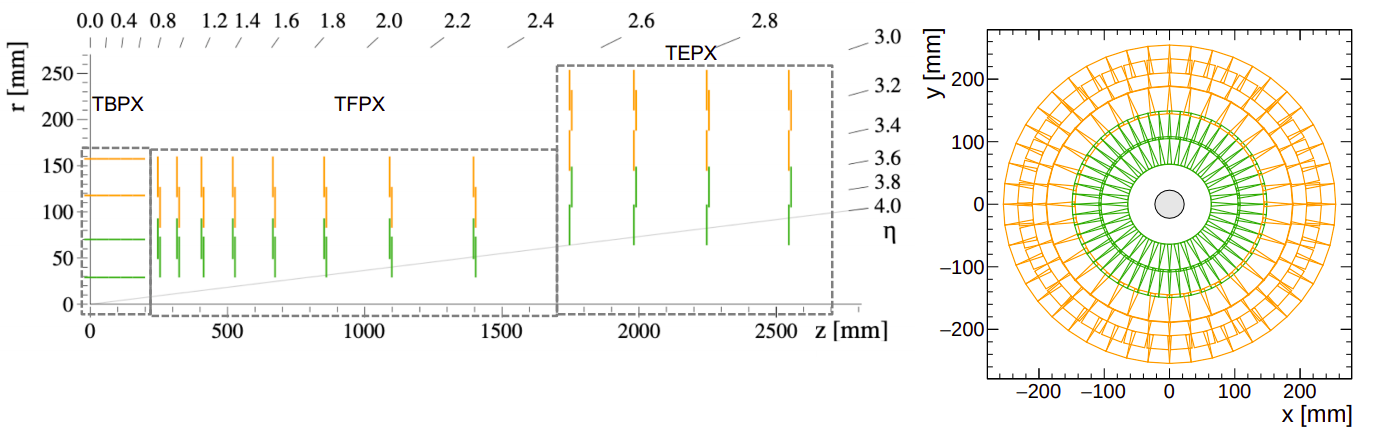
\includegraphics[width=1 \columnwidth]{ashish_thesis/tepx_tt.png}
  \caption[Phase II CMS Inner Tracker]{ \onehalfspacing Left: A layout of the CMS Phase II inner tracker showing four TEPX disks, eight TFPX disks and four barrel layers. Right: Diagram showing one double disk of TEPX with five rings.}
  \label{fig:Innertracker}
\end{figure}

%\begin{figure}[!htp]
%  \centering
 % 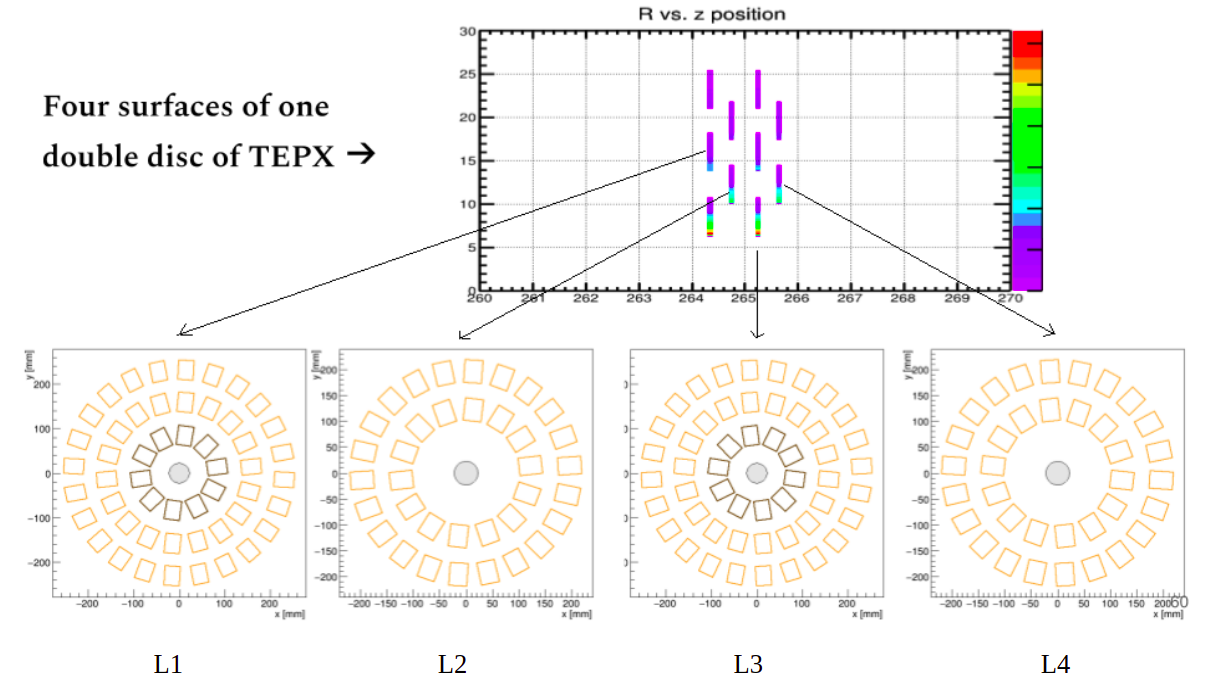
\includegraphics[width=1 \columnwidth]{ashish_thesis/fourlayers.png}
  %\caption[TEPX One Double Disk]{ \onehalfspacing Fours layers of one double disk of TEPX showing module arrangement in rings for each layer. Ring 1, 2, 3, 4 and 5 consists of 20, 28, 36, 44 and 48 modules respectively. }
  %\label{fig:CMS1_49}
%\end{figure}

\section{Phase II CMS tracker simulation samples}

 Simulated data samples for Phase II include full CMS detector description and uses official CMS software (version $\texttt{CMSSW\_10\_6\_0\_patch2}$) which calls GEANT4 for particle and energy deposit simulation as well as for reconstruction \cite{GEANT4:2002zbu}. These samples contain single-neutrino event overlaid with a variable number of minimum-bias events (events with any amount of real energy detected in CMS) to simulate different pileup values. The statistics for samples with average pileup values from 0.5 to 2 is 500000 events per step and for average pileup values between 10 and 200, statistics is 100000 as shown in Table \ref{tab:sample_12}. The number of event processed in this study for each pileup is shown in Table \ref{tab:sample_2}.

\begin{table}[ht]
  \centering
  \caption[Phase II simulated samples]{Total number of events in Phase II CMS tracker simulated samples}
  \begin{tabular}{cc}
    \textbf{pileup} & \textbf{Total number of events} \\
    \hline
    noPU  & 500000 \\
    0.5 & 500000 \\
    1 & 500000 \\
    1.5 & 500000 \\
    2 & 500000 \\
    10 & 100000 \\
    30 & 100000 \\
    50 & 100000 \\
    100 & 100000 \\
    140 & 99600 \\
    200 & 100000 \\
  \end{tabular}
  \label{tab:sample_12}
\end{table}

%The dataset is a simulated sample designed to evaluate the phase-2 upgrade of the CMS tracker. It includes a range of pileup conditions, from zero to 200 collisions per bunch crossing. Generated using a neutrino gun for events and version 10.6.0 of the CMS Software, the dataset aims to replicate conditions expected for the 2023 CMS upgrade. The data goes through a three-step process that consists of generating initial events, simulating the detector's response, and reconstructing physics objects for further study.
%Table \ref{tab:sample_1} provides information about the number of events per file in relation to  pileup. Pileup is used to denote the number of pp collisions per bunch crossing. In the table, the pileup ranges from 'noPU' (no pileup) to a pileup of 200. As the pileup increases, the number of events per file generally decreases. For example, with no pileup, there are 2000 events per file. At a pileup of 0.5, this remains the same. However, as the pileup increases to 1, the number of events drops to 1800. The decrease continues progressively until a pileup of 2, where there are 1400 events per file. Beyond a pileup of 10, the number of events per file dramatically drops and stays constant at 100 events per file for pileups from 50 to 200. The number of event processed in this study for each pileup is shown in Table \ref{tab:sample_2}.

\begin{comment}
\begin{table}[ht]
  \centering
  \caption{Events per file for each pileup}
  \begin{tabular}{ccc}
     \textbf{Pileup} & \textbf{Events per file} \\
     \hline
     noPU &   2000\\
     0.5 &   2000\\
     1&    1800\\
      1.5&  1500\\
      2&   1400\\
     10&    500\\
     30&    200\\
      50&   100\\
      100&   100\\
     140&    100\\
       200&    100\\
  \end{tabular}
  \label{tab:sample_1}
\end{table}

\end{comment}

\begin{table}[ht]
  \centering
  \caption{Events processed for each pileup}
  \begin{tabular}{ccc}
     \textbf{Pileup} & \textbf{Number of events processed} \\
     \hline
     noPU & 100000  \\
     0.5 &  100600 \\
     1&    87400\\
      1.5& 74900 \\
      2&  66200 \\
     10&   21800 \\
     30&    10000\\
      50&   5000\\
      100&   5000\\
     140&    5000\\
       200&    5000\\
  \end{tabular}
  %\caption{Events processed for each pileup}
  \label{tab:sample_2}
\end{table}

\section{Luminosity measurement using TEPX}

%Luminosity measurement for Phase II HL-LHC pixel detector will be done using two different systems: TEPX and D4R1 \cite{Haranko2023}. TEPX will be used in physics for tracking but will also get a dedicated trigger generated by the BRIL trigger board, data will be only processed by luminosity hardware of TEPX and send to BRILDAQ. D4R1 will be a dedicated luminometer with dedicated triggers fully independent of the CMS DAQ system for data analysis. Luminosity measurement using TEPX will be based on real time pixel cluster/coincidences counting (PCC) on FPGA, a method which involve counting the number of pixel clusters in the pixel detector (innermost part of the CMS tracker) per bunch crossing in minimum bias events. The innermost ring of the last disk of TEPX (D4R1) is located at 2.65 m away from the interaction point that is beyond the tracking acceptance ($|\eta| = 4$) and as this region has few tracking points, it can be solely used for the purpose of luminosity measurement by using the full available trigger rate and bandwidth \cite{Collaboration:2706512}. D4R1 will have dual purpose, luminosity and beam induced background (beam gas & beam halo) measurements. It will be operated during LHC ramp when beams are not colliding for measuring beam induced backgrounds. First bunch in a train or noncolliding bunches will be used for beam-induced background measurements.

During Phase II HL-LHC, the pixel detector's luminosity will be measured using two systems: TEPX and D4R1  \cite{Haranko2023}. TEPX, primarily for tracking in physics, will also have a dedicated BRIL trigger for luminosity data, processed and sent to BRILDAQ. D4R1, a separate luminometer, operates independently of the CMS DAQ system  \cite{Collaboration:2706512}. TEPX's luminosity measurement uses real-time pixel cluster counting (PCC) on FPGA, tracking clusters per bunch crossing in minimum bias events. D4R1, located at 2.65 m from the interaction point and beyond tracking acceptance, focuses on luminosity and beam-induced background measurements, including during non-colliding LHC ramps.

Expected CMS L1 trigger rate is around 750 kHz at pileup 200. 500 kHz trigger rate during van der meer scans (pileup 0.5) and 75 kHz (10\% of expected CMS L1 trigger rate) trigger rate will be used for TEPX luminosity measurement at pileup 200. 1000 kHz trigger rate during van der meer scans (pileup 0.5) and 825 kHz trigger rate will be used for D4R1 luminosity measurement at average pileup 200.

The TEPX and D4R1 detectors will utilize an independent BRIL trigger board (BTB) for luminosity measurement, separate from the CMS L1 trigger system. This setup includes a local control stream synchronized with the LHC clock. Data from TEPX will be transmitted via high-speed links and processed by an FPGA for pixel clustering and histogramming, ensuring synchronization with CMS's overall timing and control system.

\begin{comment}
TEPX and D4R1 will require BRIL trigger board (BTB) independent of CMS L1 trigger system to have full control over luminosity triggers, local TCDS2-like control stream for D4R1 synchronised to LHC clock, luminosity local L1 triggers, encoding of beam 1 & beam 2 logical signals. CMS Timing and Control Distribution System (TCDS) receives LHC Clock and Orbit signals that are generated by the LHC RF system and uses them for generating the CMS Clock and commands. Measurement of beam induced background with D4R1 during the LHC ramp will need to be independent but synchronized to the rest of CMS and the central services like TCDS2 and data acquisition will be implemented using special clocking scheme. Trigger and timing subsystem for D4R1 will receive a dedicated “TCDS2-like” control stream from the BRIL trigger board (BTB) that is based on the LHC clock.

Data accepted by CMS L1 trigger (750 kHz) will be collected by the end column of the pixel chip in TEPX and sent through electrical links (eLinks) at 1.28 Gb/s to LpGBT ASICs for optical transmission.
Backend system DTC will be connected to frontend TEPX electronics via low-power Gigabit Transceiver (LpGBT) optical links.
Optical down-links at 2.5 Gb/s will be used for clock, trigger, commands, and configuration data to the pixel modules.
Optical up-links at 10 Gb/s will carry readout data from L1 accept and monitoring information to the DAQ and control system.
TEPX luminosity processing will be performed by a separate luminosity processor board to which the DTC backend will send data over $~$ 4 x 25 Gb/s optical links.

TEPX luminosity processing FPGA will consist of pixel clustering and histogramming instances.
Clustering firmware will consists of
Stream decoder: It will receives TEPX chip data, separate it from data appended by DTC and decode it.
Quarter core processor: It will be used to identify up to four possible clusters within a quarter core. Two hits form a cluster if they touch horizontally, vertically or diagonally.
Quarter core distributor: The quarter core distributor will check a given quarter core for isolation and decides whether it has to be sent to the row merger or counted internally.
Count accumulator: It will receive final data bit and increment cluster count.

\end{comment}

Fig. \ref{fig:tepx_cl} shows the location of TEPX clusters in Disk 4 in the XY plane (Z is the direction of the beam) from a simulated sample with a pileup of 200. Clusters refer to groups of hits in the pixel detector. The TEPX disk in this map consists of 5 rings which are concentric rings of pixel modules at different radial distances from the beamline.

\begin{figure}[!htp]
  \centering
  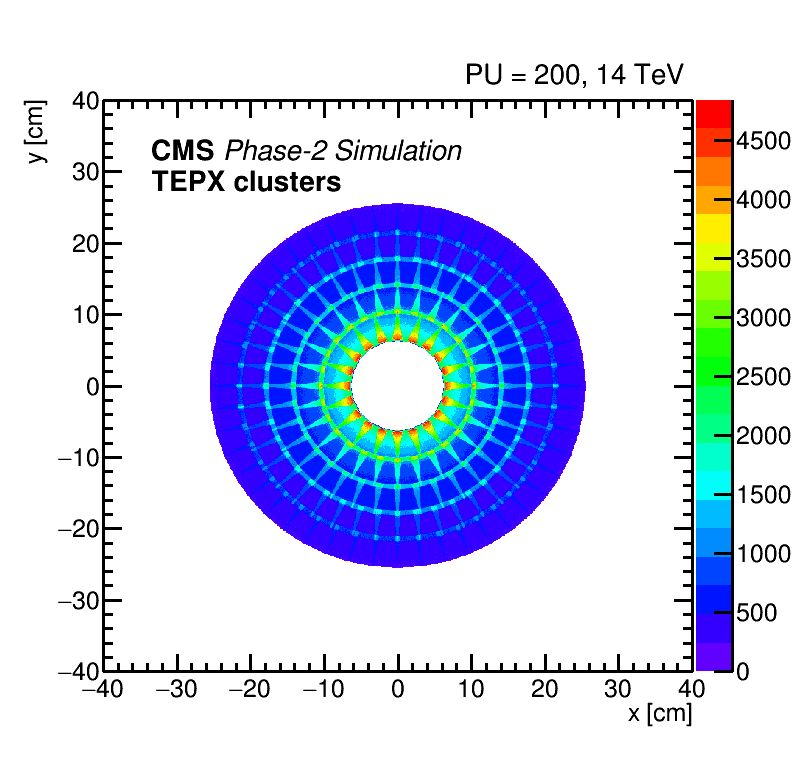
\includegraphics[width=0.9\columnwidth]{ashish_thesis/tepx_clusters_1.png}
  \caption[TEPX Cluster Map]{TEPX cluster map in the XY plane for pileup 200 simulated sample. Map showing coordinates of TEPX clusters in CMS global coordinate system. It shows clusters in one TEPX disk consisting of 5 rings. Hot regions are showing the module overlap for all rings (red, orange, green, yellow). Number of x bins is 1000, x bins range from -40 to 40. x bin size is 0.1 cm. Number of y bins is 1000, y bins range from -40 to 40. y bin size is 0.1 cm.}
  \label{fig:tepx_cl}
\end{figure}

The number of clusters per pp collision in Disk 4 Ring 1 varies from 0 to 2600 as a function of pileup. At pileup 200, mean number of cluster per pp collision is 2200 as shown in Fig. \ref{fig:tepx_cl_allPU}. The peak of the distribution drops as pileup increases because we have processed different number of events for different pileup values. Under low pileup conditions which is crucial for vdM calibration, number of clusters varies from 0 to 35. For average pileup value of 0.5 (vdM conditions), number of clusters varies between 0 and 12.

\begin{figure}[!htp]
  \centering
  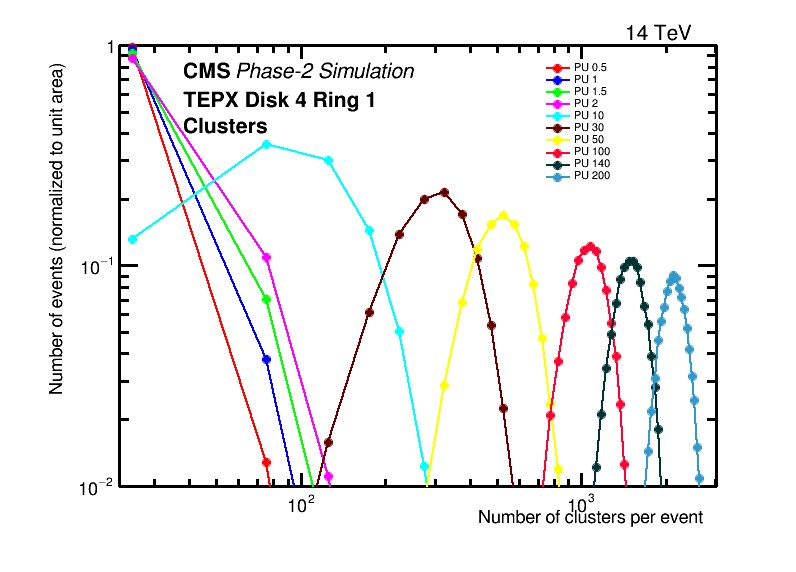
\includegraphics[width=1\columnwidth]{ashish_thesis/tepx_D4R!_clusters._allpu_1.png}
  \caption[D4R1 Clusters All Pileup]{Distribution of number of clusters for TEPX Disk 4 Ring 1 for all pileup values.}
  \label{fig:tepx_cl_allPU}
\end{figure}


Linearity is one of the systematic uncertainty in the calculation of instantaneous luminosity and PCC visible cross section $\sigma_{vis}$. A linear relation between the number of clusters and pileup (PU) imply that \\

$<N_{cl/pp}> = \frac{<N_{cl}>}{\mu} = \frac{\sigma_{vis}}{\sigma_{pp}}$ \\

$<N_{cl}> =  \frac{\sigma_{vis}}{\sigma_{pp}} \mu $ \\

Linearity indicates that the PCC visible cross section $\sigma_{vis}$ does not depend on the per bunch instantaneous luminosity (ideal luminometer). In ideal scenario, $\sigma_{vis}$ is not dependent on pileup, but this a potential problem with the luminometer. Linearity results for simulated TEPX clusters from low to high pileup values are shown from Fig. \ref{fig:CMS_420} to Fig. \ref{fig:CMS_005}. TEPX luminometer proposed for Phase II shows excellent linearity over entire pileup range. A non-linear relation $<N_{cluster}> = \alpha (PU)^{\gamma}, \gamma \neq 1$ would add non-linear terms in the rate equation $R = \sigma_{vis} L_{inst}$  and cause $\sigma_{vis}$ to vary with the per bunch instantaneous luminosity and pileup values.


\begin{figure}[H]
  \centering
  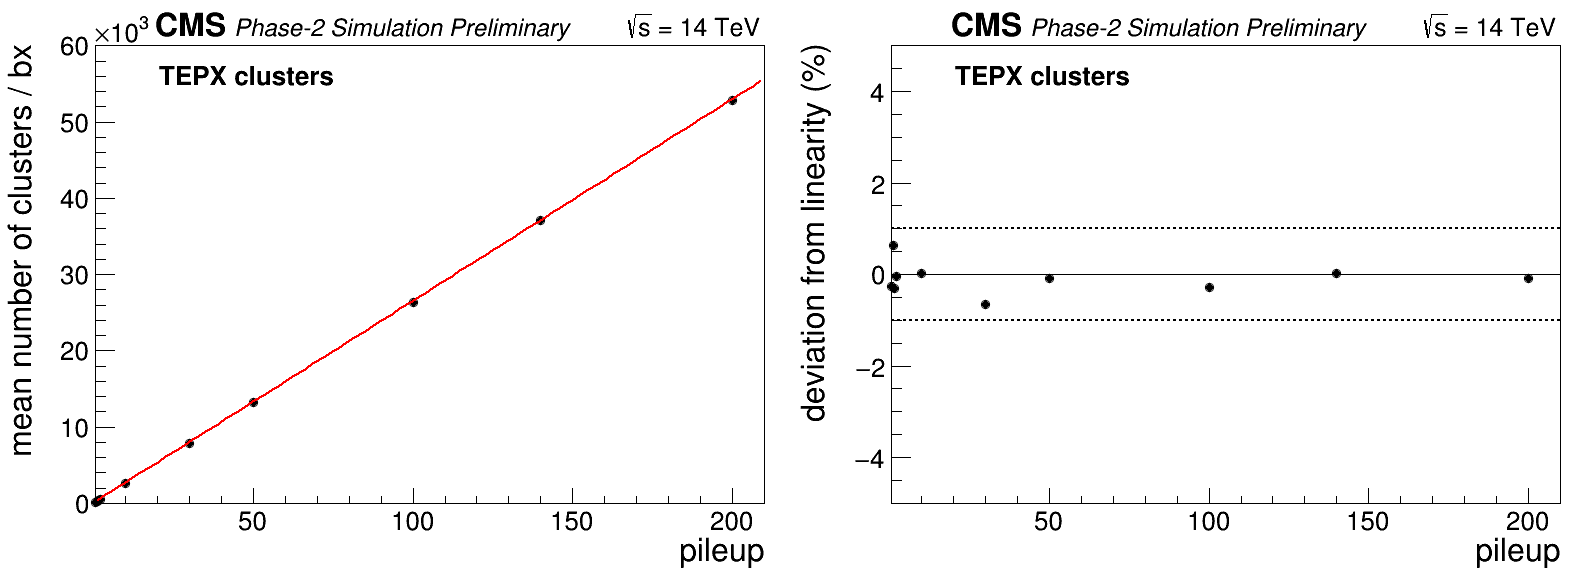
\includegraphics[width=1\columnwidth]{ashish_thesis/totalclusters.png}
  \caption[TEPX Clusters Fit And Residuals]{\onehalfspacing Left: Simulated mean number of clusters for all entire TEPX detector as a function of pileup. A line is fitted between pileup values of 0 and 2, and then extrapolated up to a pileup of 200. Right: Deviation from linearity for clusters for entire TEPX detector. The non-linearity is calculated as the relative difference between the data points and the values of the fit function at the respective pileup value. Non-linearity is within 1 \% for entire pileup range. Pileup 200 corresponds to High Luminosity (HL)-LHC environment.}
  \label{fig:CMS_420}
\end{figure}


\begin{figure}[H]
  \centering
  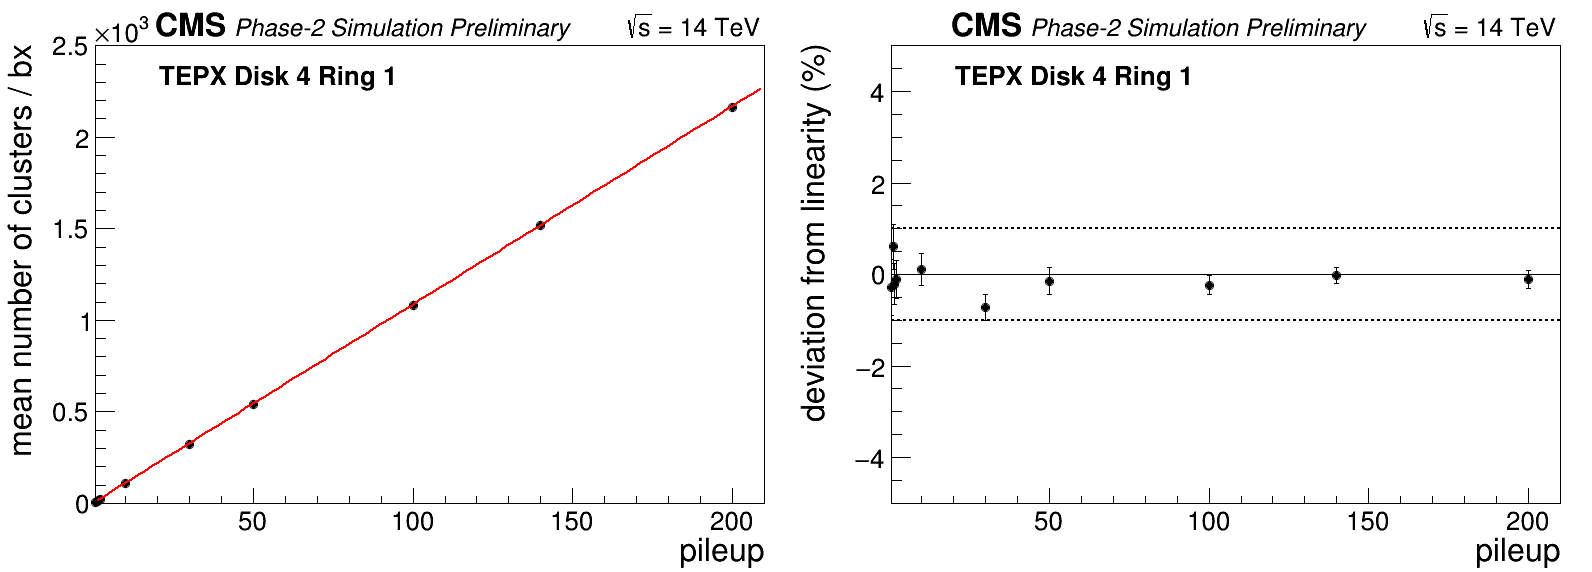
\includegraphics[width=1\columnwidth]{ashish_thesis/clustersD4R1.png}
  \caption[Disk 4 Ring 1 Clusters Fit And Residual]{\onehalfspacing Left: Simulated mean number of clusters for TEPX Disk 4 Ring 1 as a function of pileup. Right: Deviation from linearity for clusters for TEPX Disk 4 Ring 1. The non-linearity is calculated as the relative difference between the data points and the values of the fit function at the respective pileup value.}
  \label{fig:CMS_003}
\end{figure}



\begin{figure}[H]
  \centering
  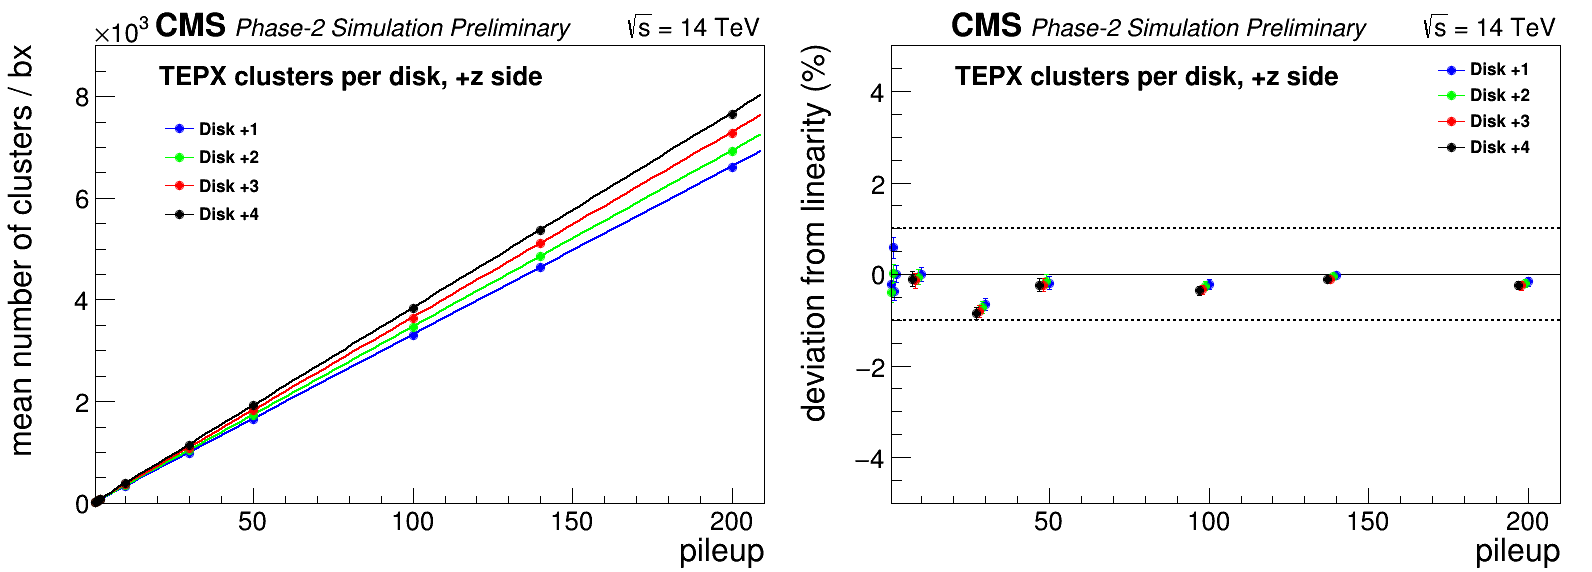
\includegraphics[width=1 \columnwidth]{ashish_thesis/clustersperdisk+z.png}
  \caption[Clusters Per disk Fit And Residual]{Left: Simulated mean number of clusters for +z side TEPX disks as a function of pileup. Right: Deviation from linearity for clusters for +z side TEPX disks.}
  \label{fig:CMS_004}
\end{figure}


\begin{figure}[H]
  \centering
  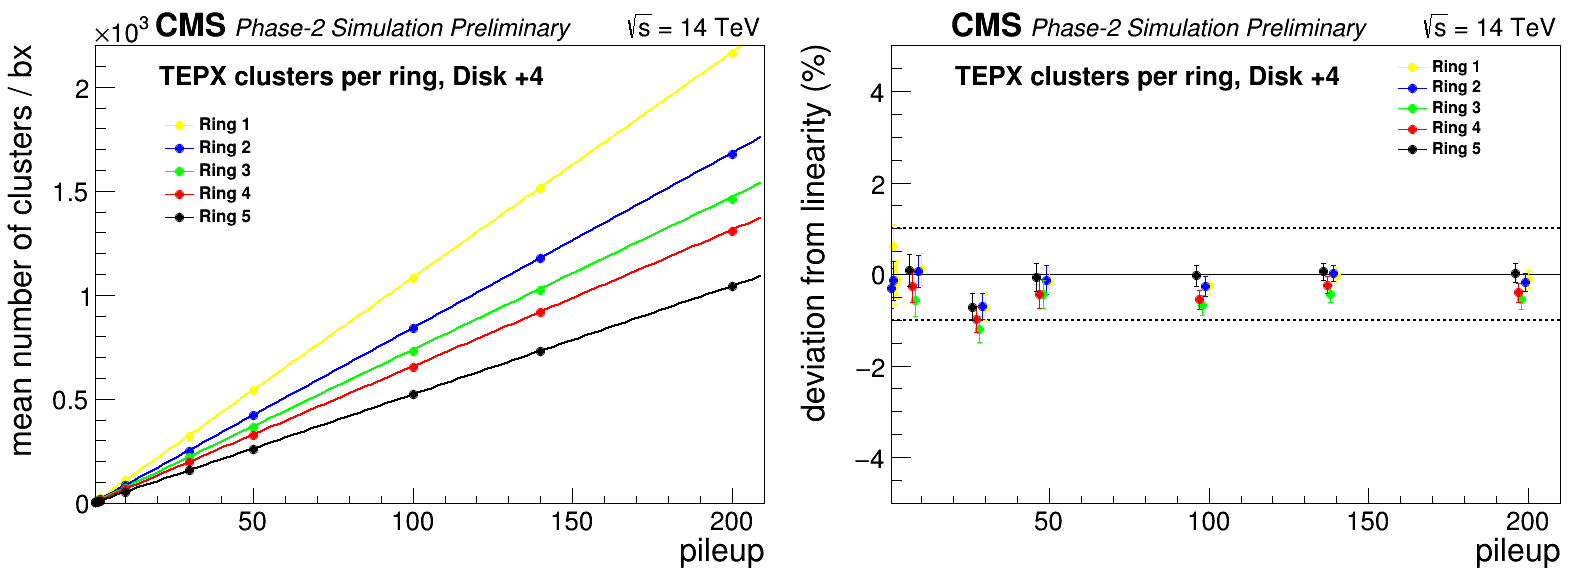
\includegraphics[width=1\columnwidth]{ashish_thesis/clustersperringD+4.png}
  \caption[Clusters Per Ring For Disk 4 Fit And Residual]{Left: Simulated mean number of clusters for +z side TEPX Disk 4 all rings as a function of pileup. Ring 1 has highest slope and Ring 5 has least slope. Right: Deviation from linearity for clusters for TEPX Disk +4 all rings. Non-linearity is within $1\%$ for all rings over entire pileup range.}
  \label{fig:CMS_005}
\end{figure}


Two fold coincidences are clusters in modules overlap regions formed by modules in front and back layers of TEPX disk. There are two types of two fold coincidences namely in phi and r. Two fold coincidence in phi involve modules overlap in the same ring  of one double disk and two fold coincidence in r require modules overlap between successive rings of one double disk.  wo fold coincidences are better way to distinguish between a real hit and random electrical noise. They are more likely to be real hit than random electrical noise. Luminosity determination based on counting coincidences has an advantage over clusters that afterglow effects are tiny in the case of coincidences. %as shown in Fig. \ref{fig:cluster_ring_4000}. 
 %(shown in Fig. \ref{fig:cluster_ring_73})
  %as depicted in Fig. \ref{fig:cluster_ring_74}. 
 %Overlap between L1 L3 and L2 L4 layers also possible but we havent considered them in this simulation. L1L2 two fold coincidences in r are clusters in module overlaps between adjacent rings in first two layers. L3L4 two fold coincidences in r are modules overlaps in the last two layers between adjacent rings. All types of two fold coincidences in r are shown in Table \ref{tab:twofoldinr}. Module overlap between different rings for all types of two fold coincidences in r are shown in Fig. \ref{tab:twofoldinr}. Two fold coincidences are better way to distinguish between a real hit and random electrical noise. They are more likely to be real hit than random electrical noise. Luminosity determination based on counting coincidences has an advantage over clusters that afterglow effects are tiny in the case of coincidences.

\begin{comment}

\begin{figure}[!htp]
\centering
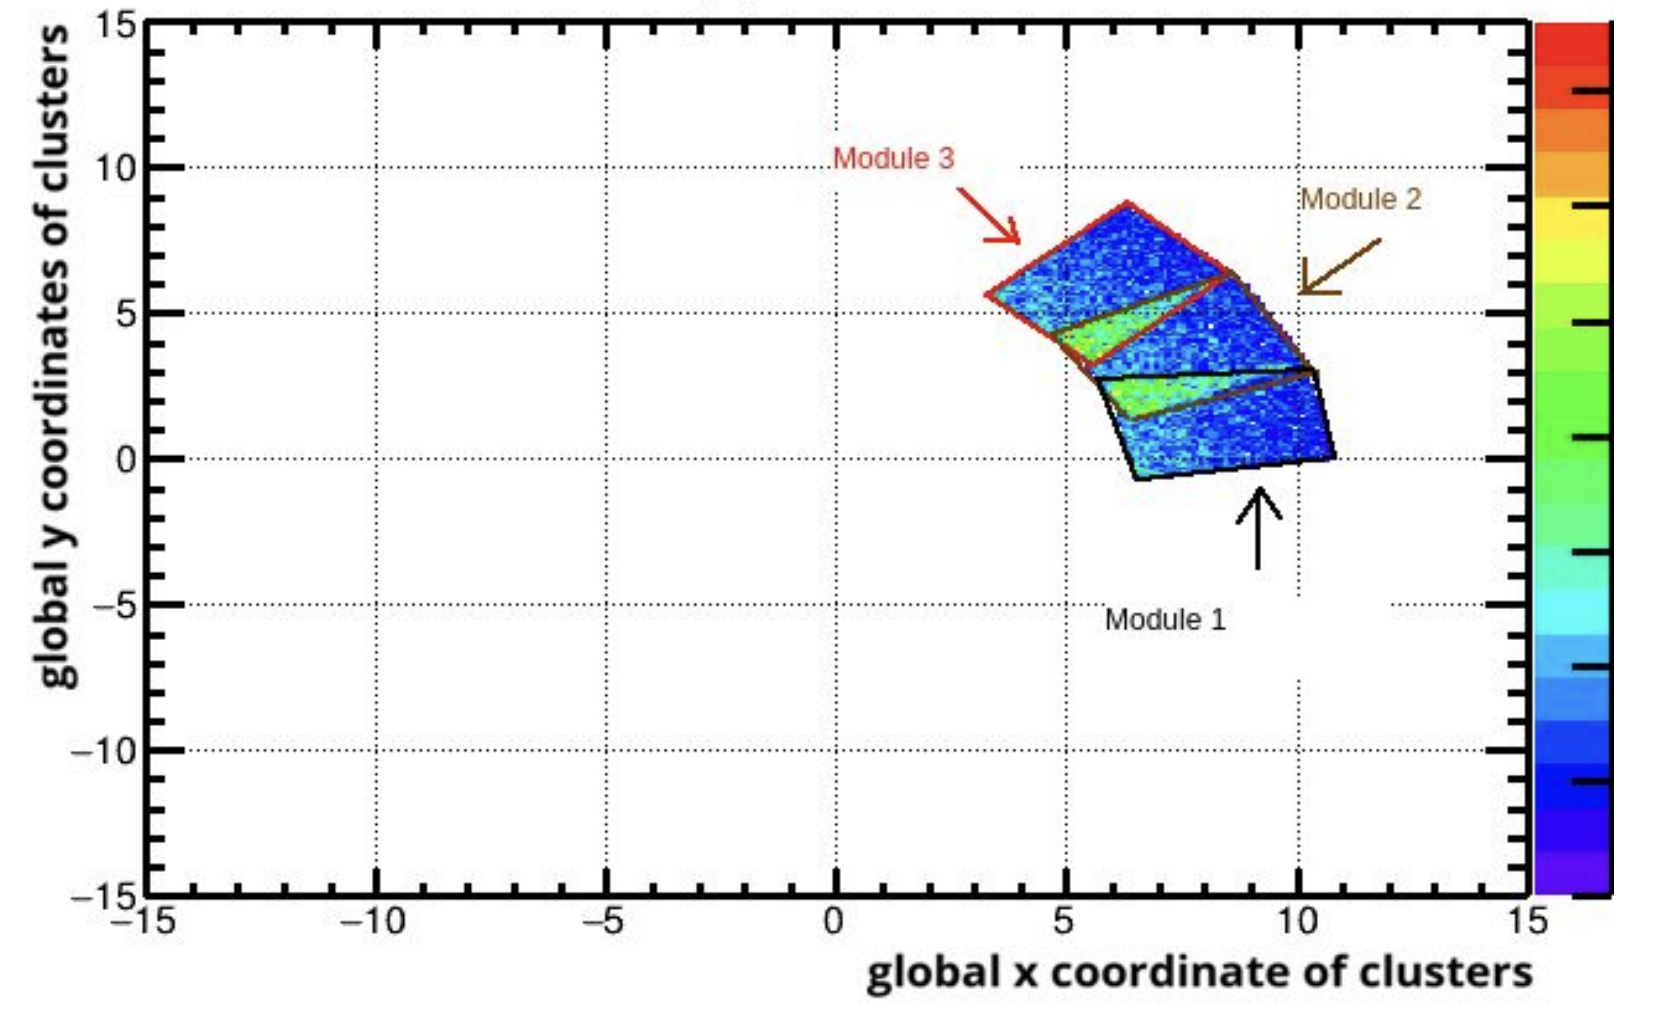
\includegraphics[width=0.6\textwidth]{ashish_thesis/twofoldinphi.png}
\caption[Module Overlap Two Fold Coincidences in phi]{%                                                                                                                                     
  Example of module overlap between same ring modules that can give rise to two fold coincidences in phi.
}
\label{fig:cluster_ring_4000}
\end{figure}

\begin{table}[ht]
  \centering
  \caption{Location of four layers in Disk 4}
\begin{tabular}{cc}
\textbf{Layer} & \textbf{z coordinate} \\ 
\hline
Layer 1 (L1) & 264.4 \\ 
Layer 2 (L2) & 264.8 \\ 
Layer 3 (L3) & 265.2 \\ 
Layer 4 (L4) & 265.6 \\ 
\end{tabular}
\label{tab:alllayerz}
\end{table}

\begin{table}[ht]
  \centering
  \caption{Types of two fold coincidences in r}
\begin{tabular}{ccc}
\textbf{Type of two fold coincidences in r} & \textbf{Module overlap} & \textbf{dz} \\ 
\hline
A & R1L1-R2L2 & 0.4 \\ 
B & R1L1-R2L4 & 1.2 \\ 
C & R1L3-R2L4 & 0.4 \\ 
D & R2L2-R3L3 & 0.4 \\
E & R3L1-R2L2 & 0.4 \\ 
F & R3L3-R2L4 & 0.4 \\ 
G & R3L1-R4L2 & 0.4 \\ 
H & R3L1-R4L4 & 1.2 \\ 
I & R3L3-R4L4 & 0.4 \\ 
J & R5L1-R4L2 & 0.4 \\ 
K & R4L2-R5L3 & 0.4 \\ 
L & R5L3-R4L4 & 0.4 \\ 
\end{tabular}
\label{tab:twofoldinr}
\end{table}

\begin{figure}[!htp]
\centering
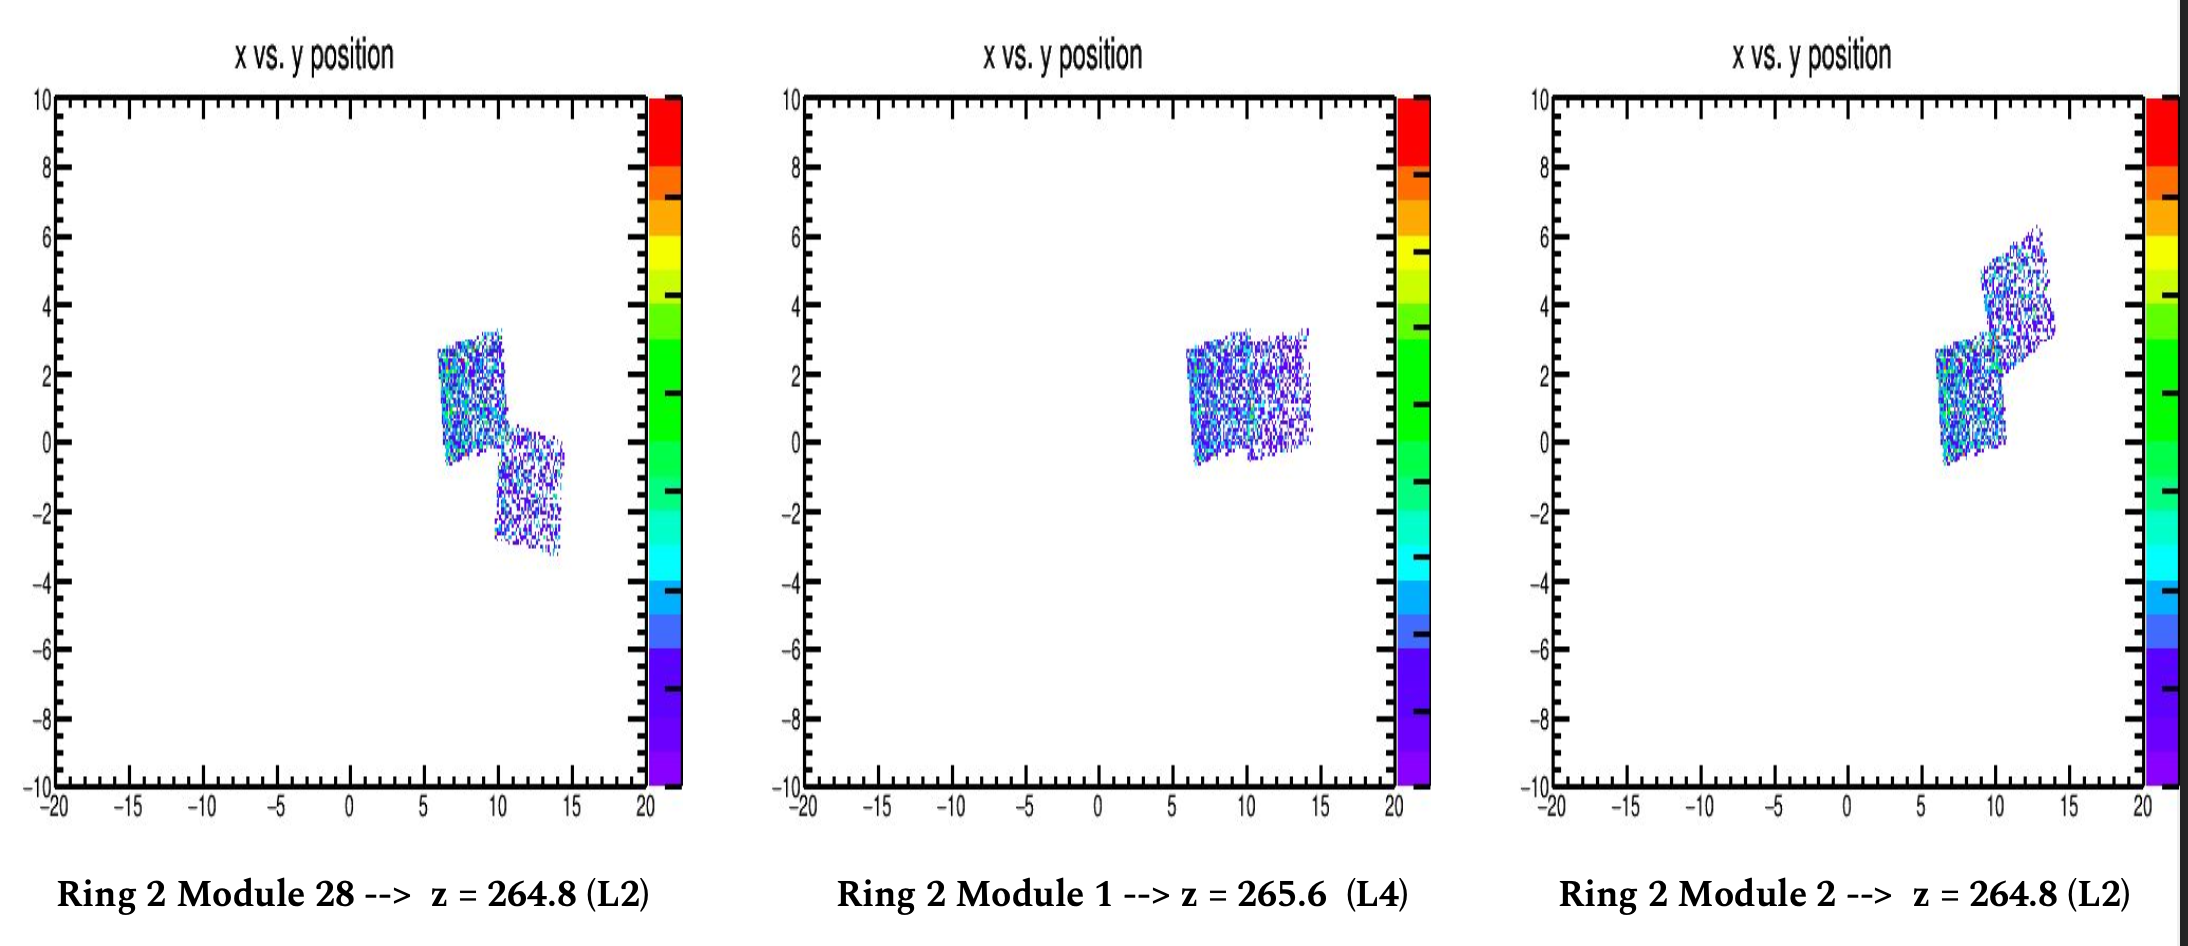
\includegraphics[width=1\textwidth]{ashish_thesis/moduleoverlapinR_1.png}
\caption[Module Overlap Two Fold Coincidences in r]{%                                                                                                                                                                         
  Example of module overlap between different ring modules that can give rise to two fold coincidences in r.
}
\label{fig:cluster_ring_73}
\end{figure}

\begin{figure}[!htp]
\centering
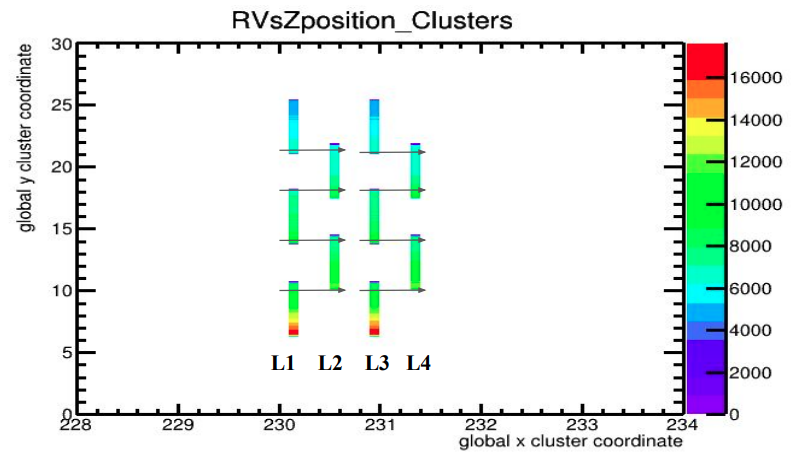
\includegraphics[width=1\textwidth]{ashish_thesis/twofoldinRmethod.png}
\caption[Few types Of Two Fold Coincidences in r]{%                                                                                                                                                                              
  Example of module overlap between different ring modules in the first two and last two layers of one tepx double disk that can give rise to two fold coincidences in r.
}
\label{fig:cluster_ring_74}
\end{figure}

\end{comment}


%\begin{figure}[!htp]
 % \centering
  %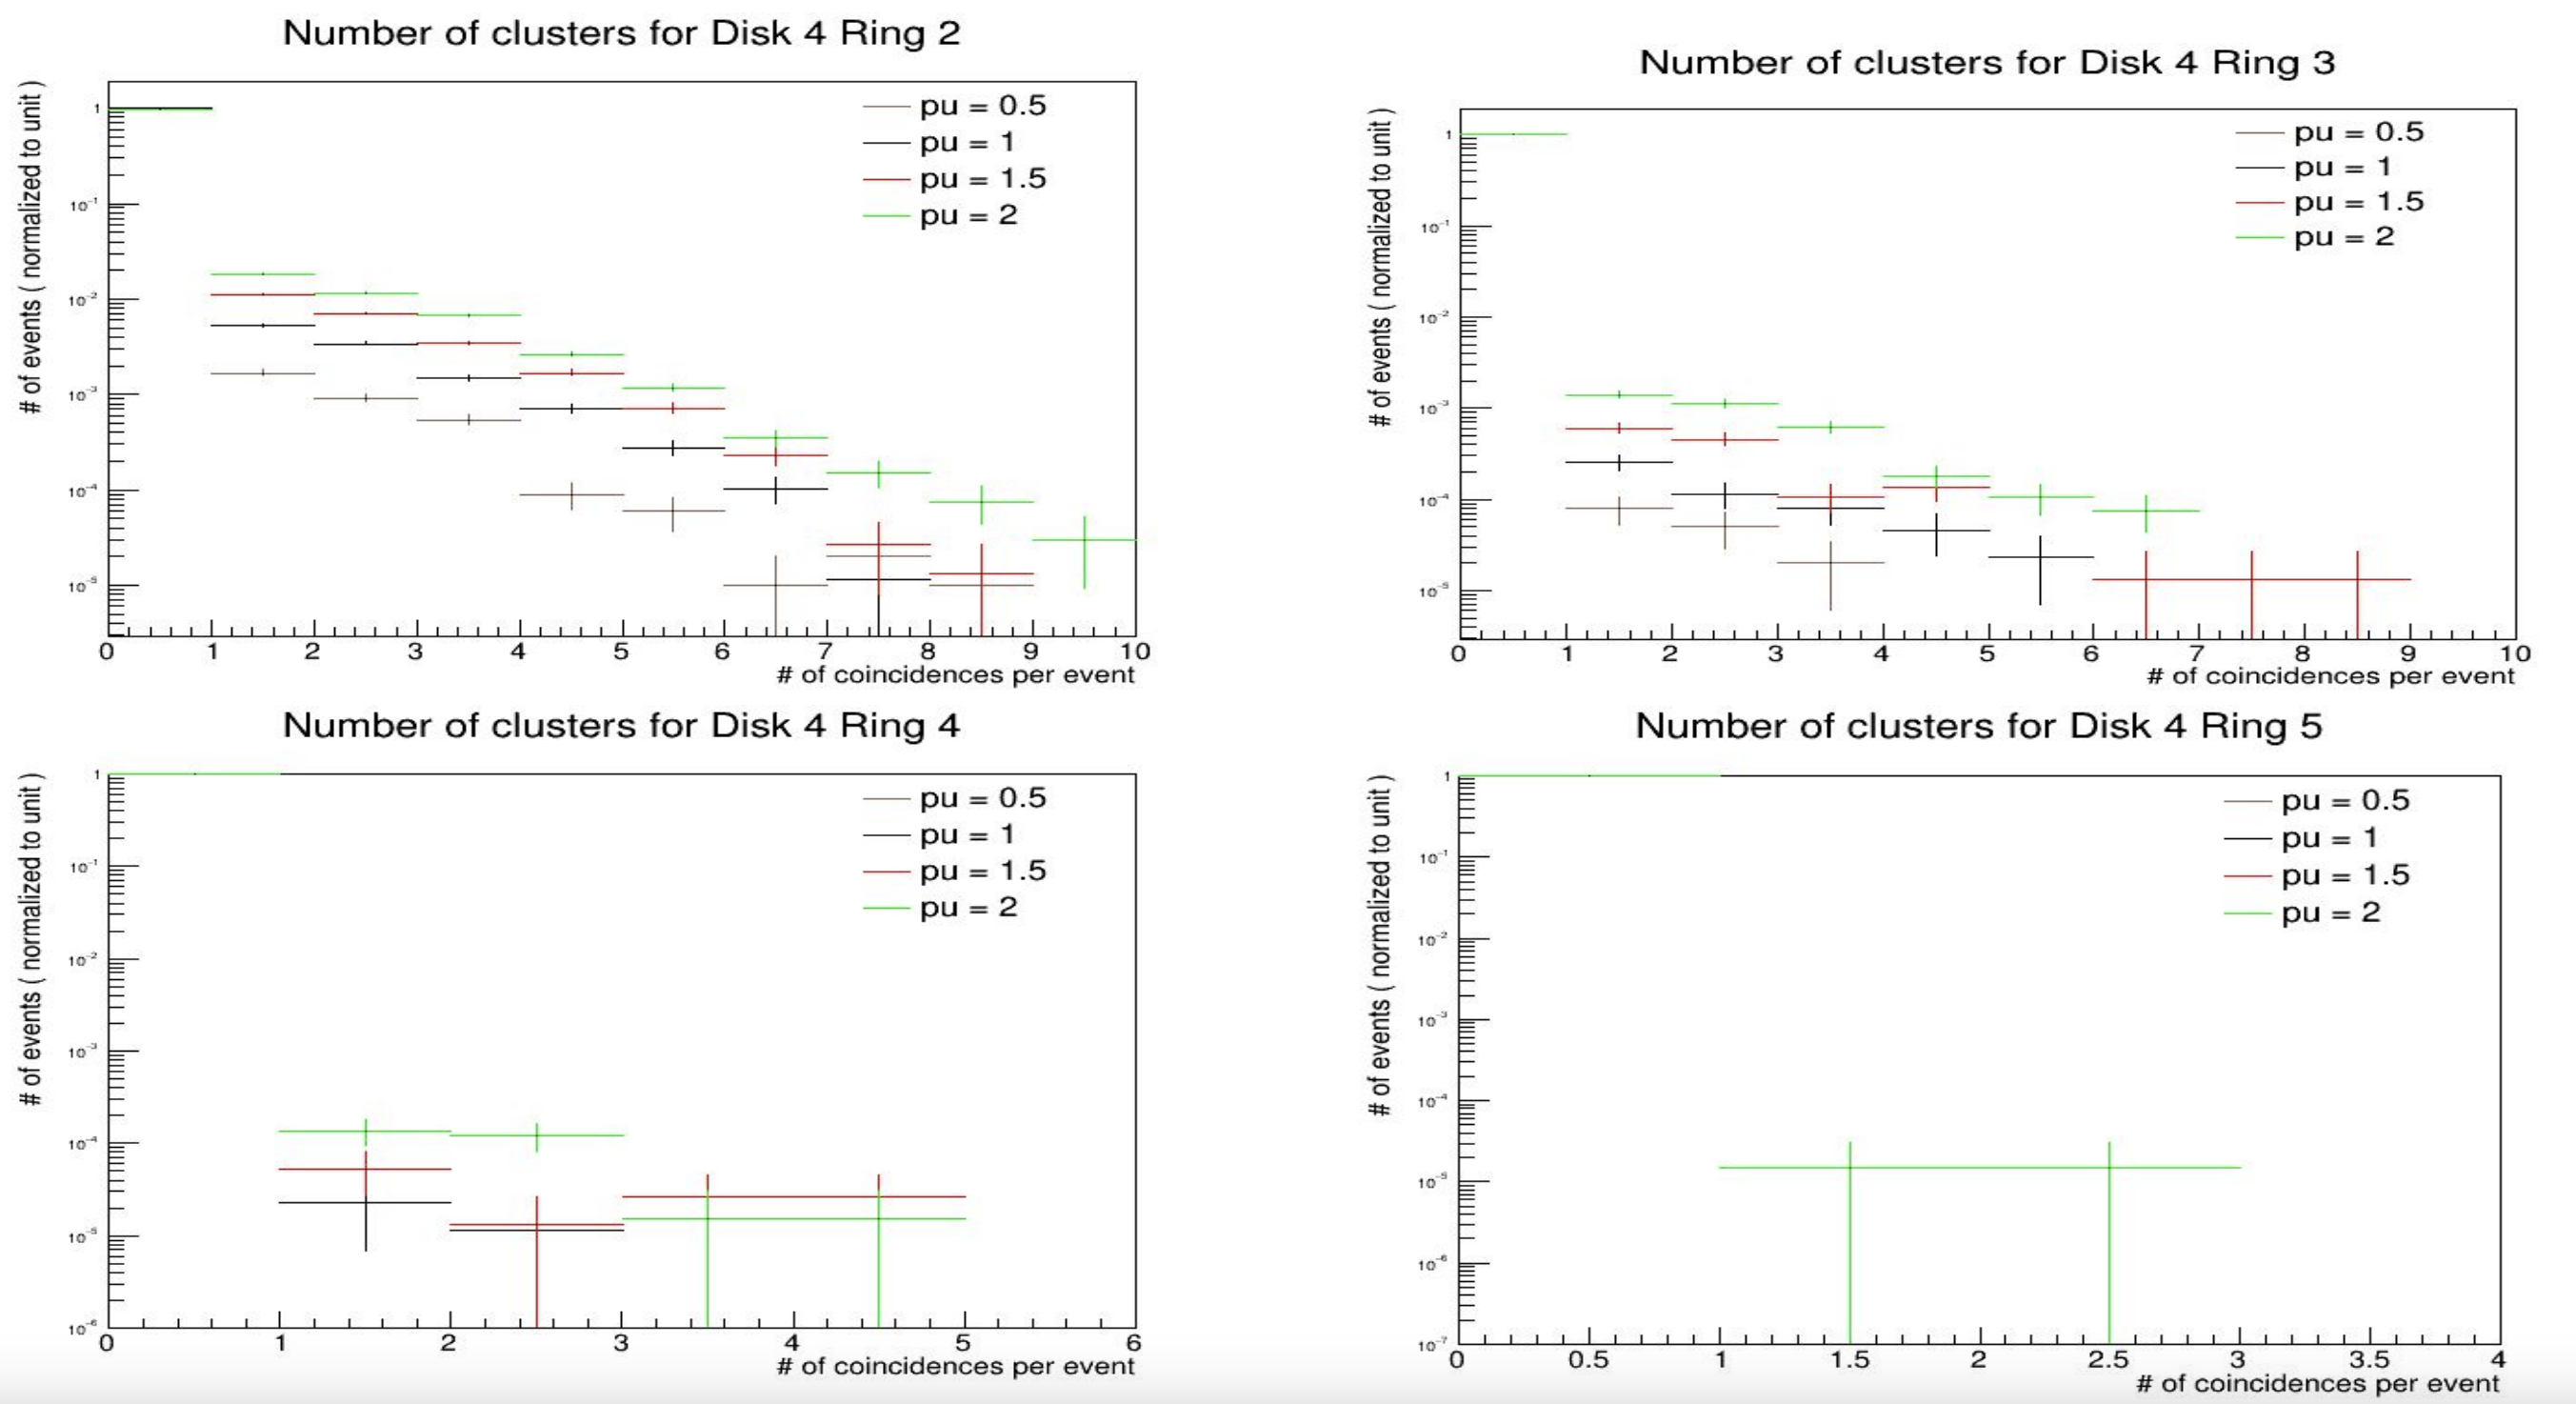
\includegraphics[width=1\columnwidth]{ashish_thesis/tepx_D4_3foldcoin_lowpu.png}
  %\caption[TEPX D4 All Rings Three Fold Coincidences Low Pileup]{Distribution of number of three fold coincidences for TEPX Disk 4 all rings for low pileup values.}
  %\label{fig:tepx_3foldcoin_lowPU}
%\end{figure}

\begin{comment}

The old algorithm for defining two fold coincidence employ x and y global position coordinates of clusters \cite{dabrowski2020}. Separation between x and y coordinate of original and coincidence cluster with proper selection and z coordinate selection in accordance with the separation between different layers in tepx disk is used as shown in Fig. \ref{fig:oldvar_xy}.

dx=x2-x1, dy=y2-y1

\begin{itemize}

\item Two fold coincidence in this algorithm is defined as the pair of hits in the module overlap region within TEPX disk satisfying dx and dy selections of 0.1 and separated by z coordinate of 0.9.

\item True coincidences are hits in module overlap region satisfying dx, dy selections of 0.1 and generated by same simulated track id.

\item Fake coincidences are hits in module overlap region satisfying same dx, dy selections of 0.1 but not generated by same simulated track id.

\end{itemize}

\begin{figure}[!htp]
\centering
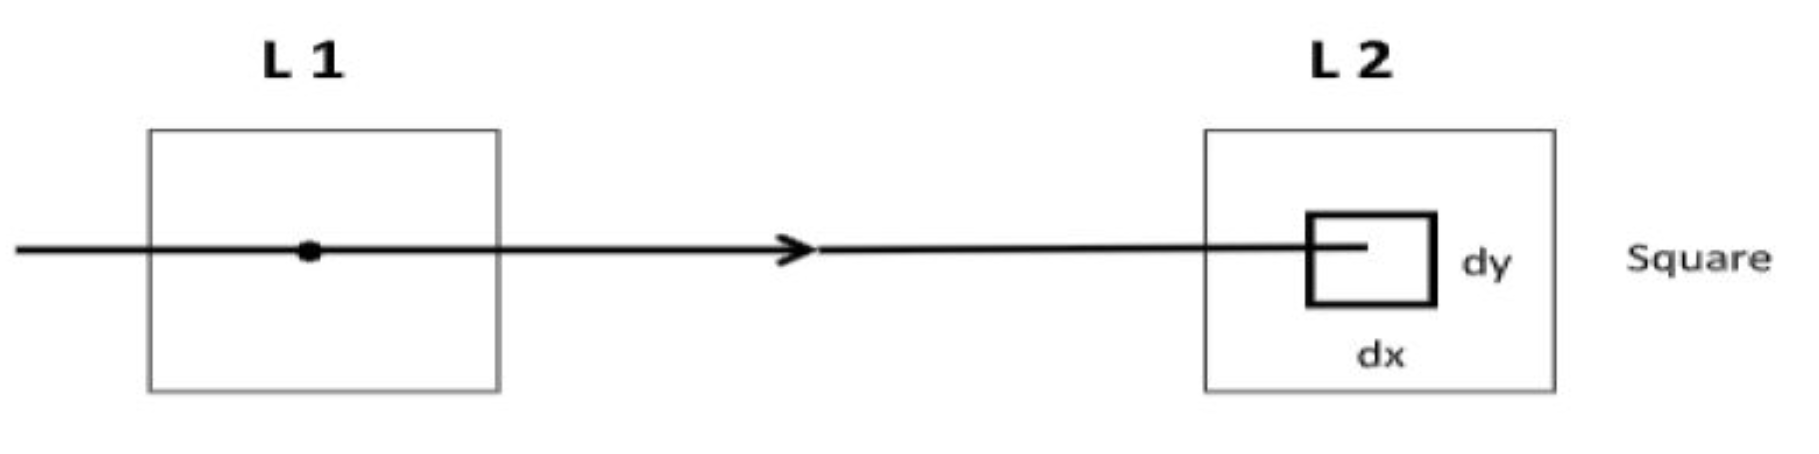
\includegraphics[width=1\textwidth]{ashish_thesis/oldvariable_xy.png}
\caption[Old Definition Of Two Fold Coincidences]{%
   Old x, y variables used for defining two fold coincidences clusters in phi.
}
\label{fig:oldvar_xy}
\end{figure}


\begin{figure}[!htp]
\centering
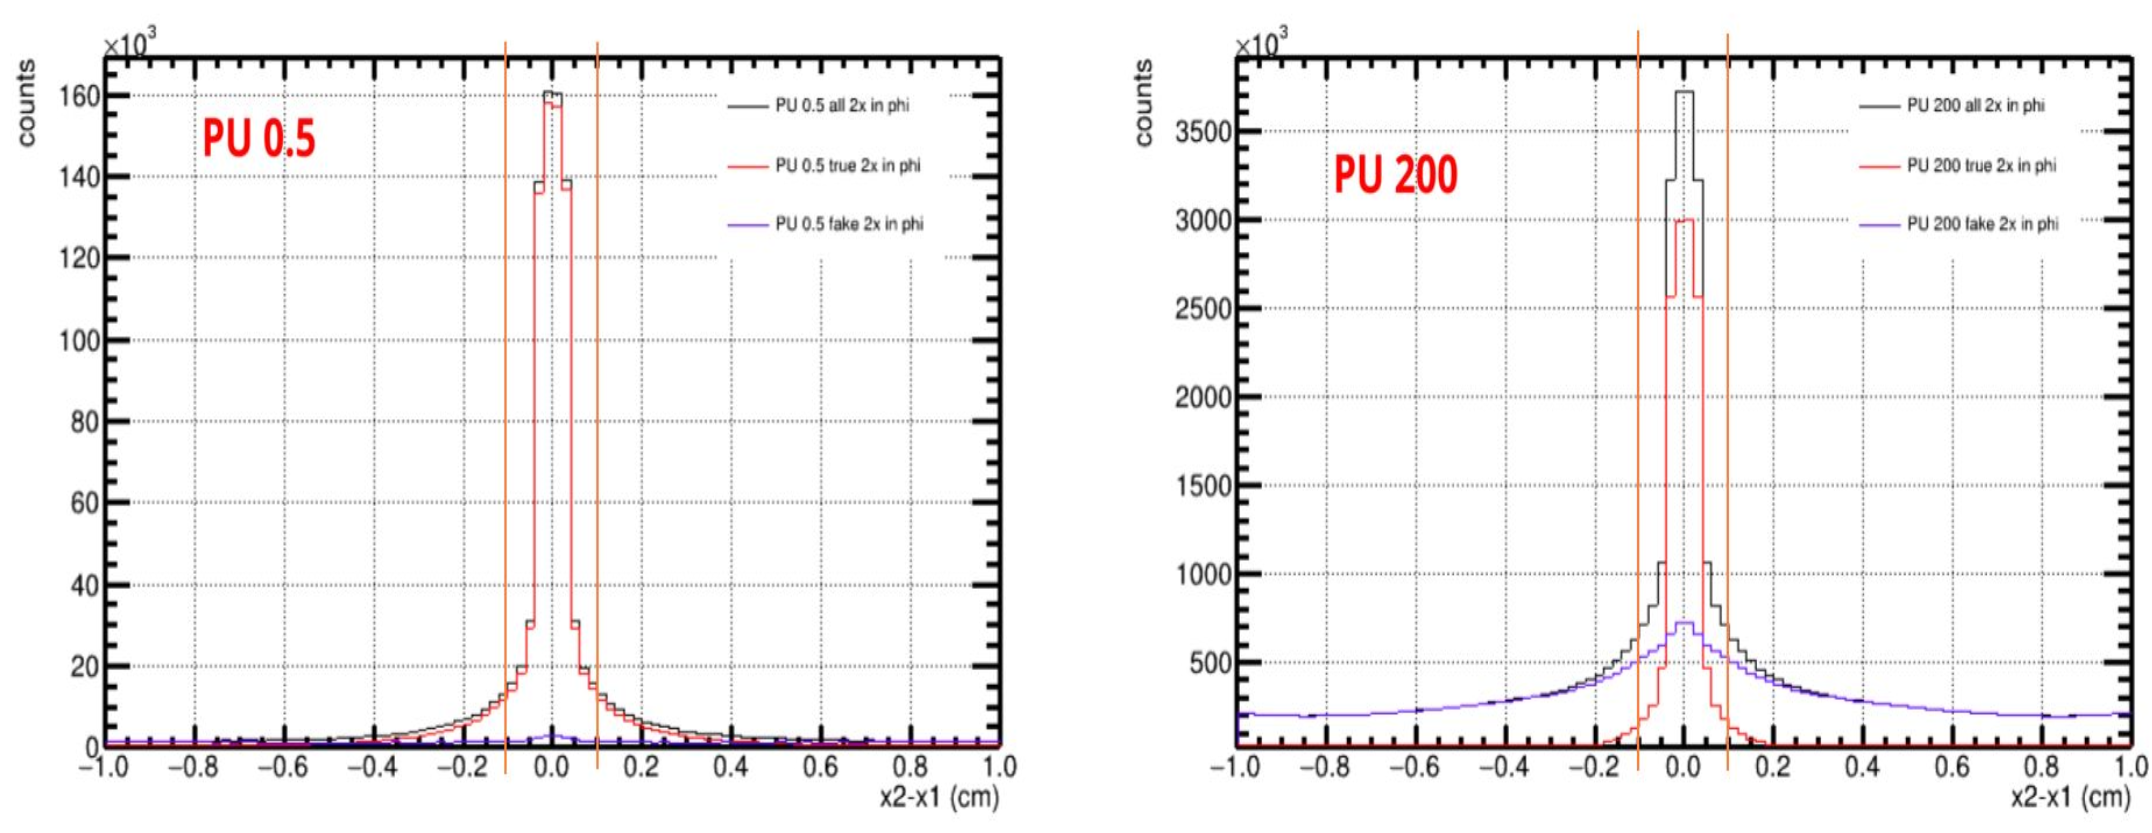
\includegraphics[width=1\textwidth]{ashish_thesis/twofoldcoin_inphi_PU0p5_200.png}
\caption[Total, True and Fake Two Fold coincidences in phi (old x variables)]{%
 Separation between x coordinates of clusters in module overlap region for pileup 0.5 and 200 showing distribution total, true and fake two fold coincidences in phi.
}
\label{fig:dx_twofold}
\end{figure}


\begin{figure}[!htp]
\centering
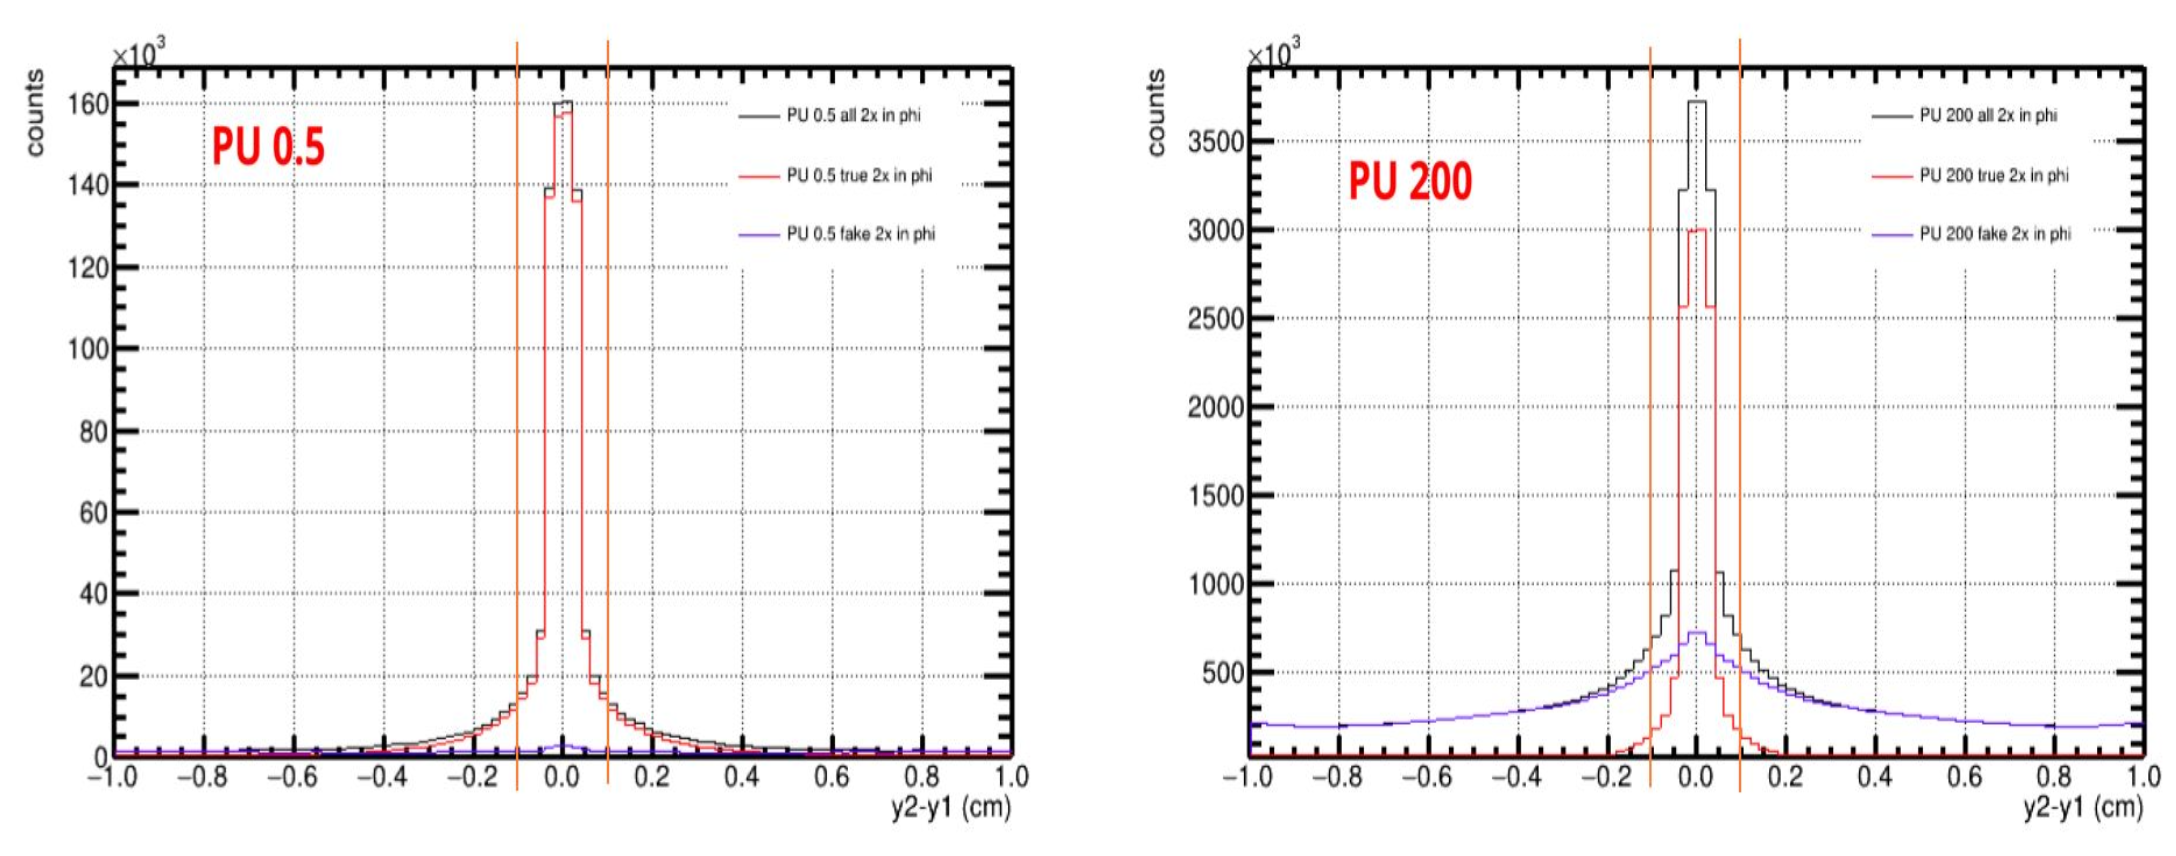
\includegraphics[width=1\textwidth]{ashish_thesis/twofoldcoin_cluster_y.png}
\caption[Total, True and Fake Two Fold Coincidences in phi (old y variables)]{%
    Separation between y coordinates of clusters in module overlap region for pileup 0.5 and 200 showing distribution total, true and fake two fold coincidences in phi.
}
\label{fig:dy_twofold}
\end{figure}

In order to reduce fake two fold coincidences for high pileup, we tried more stringent selections on separation of x, y variables for original and coincidence clusters as depicted in Fig. \ref{fig:cutopdxdy} to select dx, dy distribution (shown in Fig. \ref{fig:dx_twofold} and Fig. \ref{fig:dy_twofold}) only close to the peak cluster count but were unable to improve the residuals at high pileup to suppress physics noise. With this algorithm, we obtain residual upto 3\% even with smallest possible selection on dx and dy. Residuals obtained using different value of dx, dy selections are shown in Fig. \ref{fig:res_dxdycut}.

\begin{figure}[!htp]
\centering
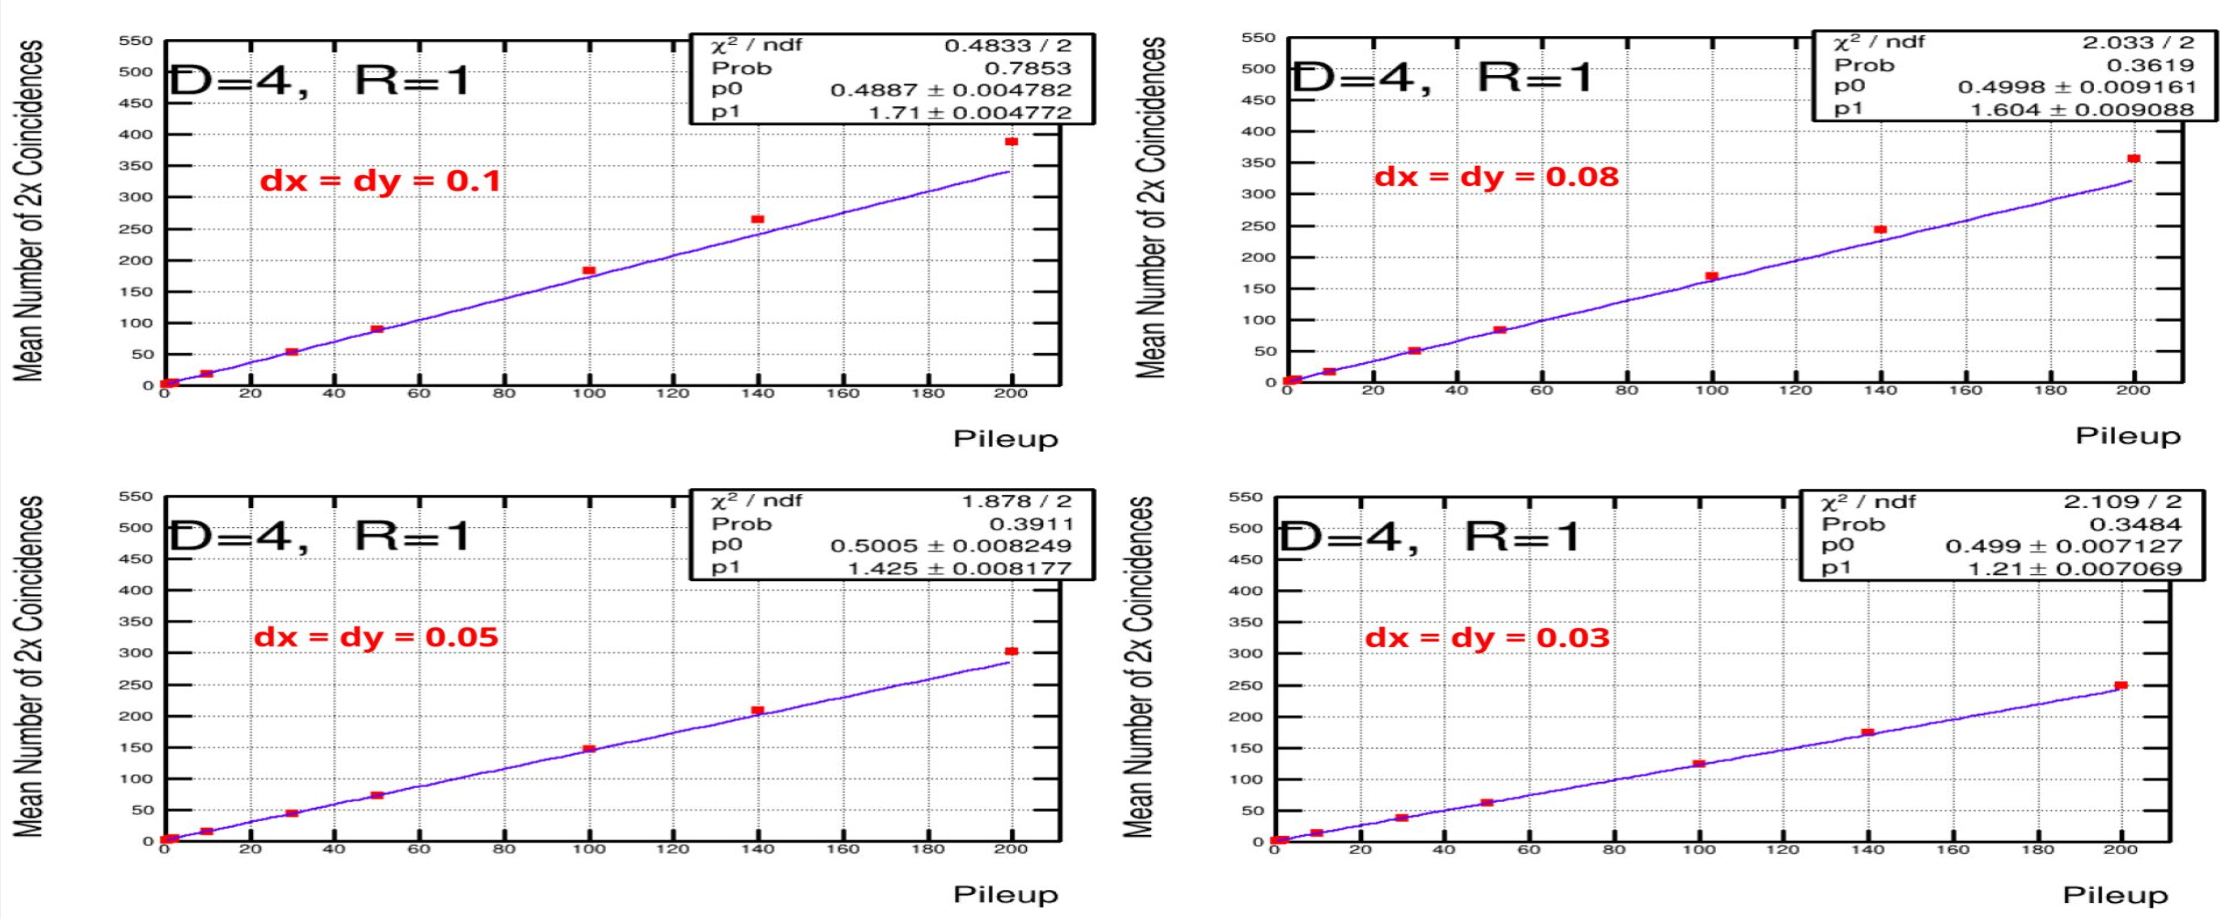
\includegraphics[width=1\textwidth]{ashish_thesis/cut_optimization_twofoldcoin.png}
\caption[Cut Optimization  Old variables]{%
 Cut optimization for two fold coincidences based on x, y variables to compute coincidence cluster separation.
}
\label{fig:cutopdxdy}
\end{figure}

\begin{figure}[!htp]
\centering
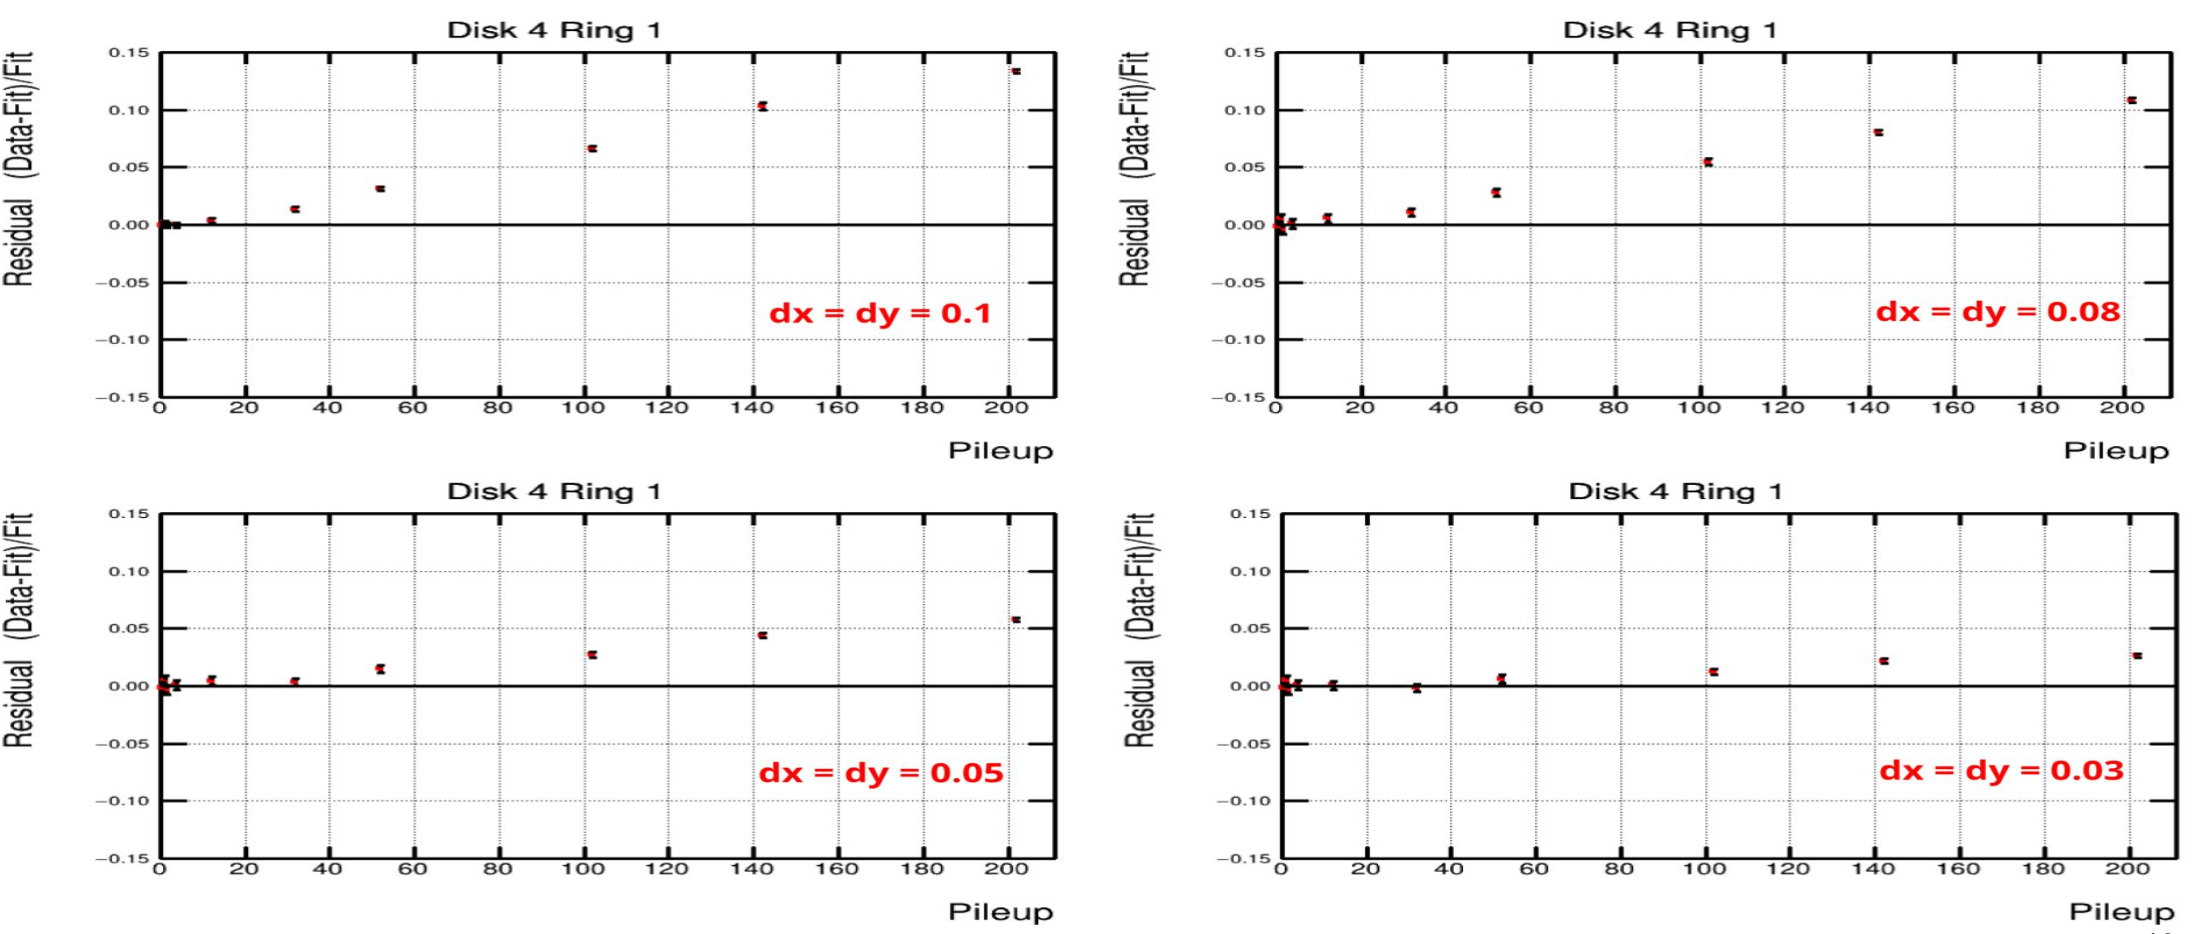
\includegraphics[width=1\textwidth]{ashish_thesis/cut_optimization_residual.png}
\caption[Residuals Different Cut Values]{%
  Residual obtained after doing linear fit for different values of dx and dy. Fake two fold coincidences does not show decrement for high pileup when more stringent selections are applied on dx, dy variables.
}
\label{fig:res_dxdycut}
\end{figure}

\end{comment}

\newpage
A new algorithm for luminosity measurement based on counting two fold coincidences is proposed that applies selections using dr and $d\phi$ variables (shown in Fig. \ref{fig:drdphi_diagram}) to minimize non-linearity for high pileup as these variables take into account track angle and its curvature \cite{sehrawat2020}.  Proper selections are applied for each TEPX disk based on these variables using low pileup simulated samples and then these selections are extrapolated to high pileup samples for suppressing fake coincidences.


\begin{figure}[!htp]
\centering
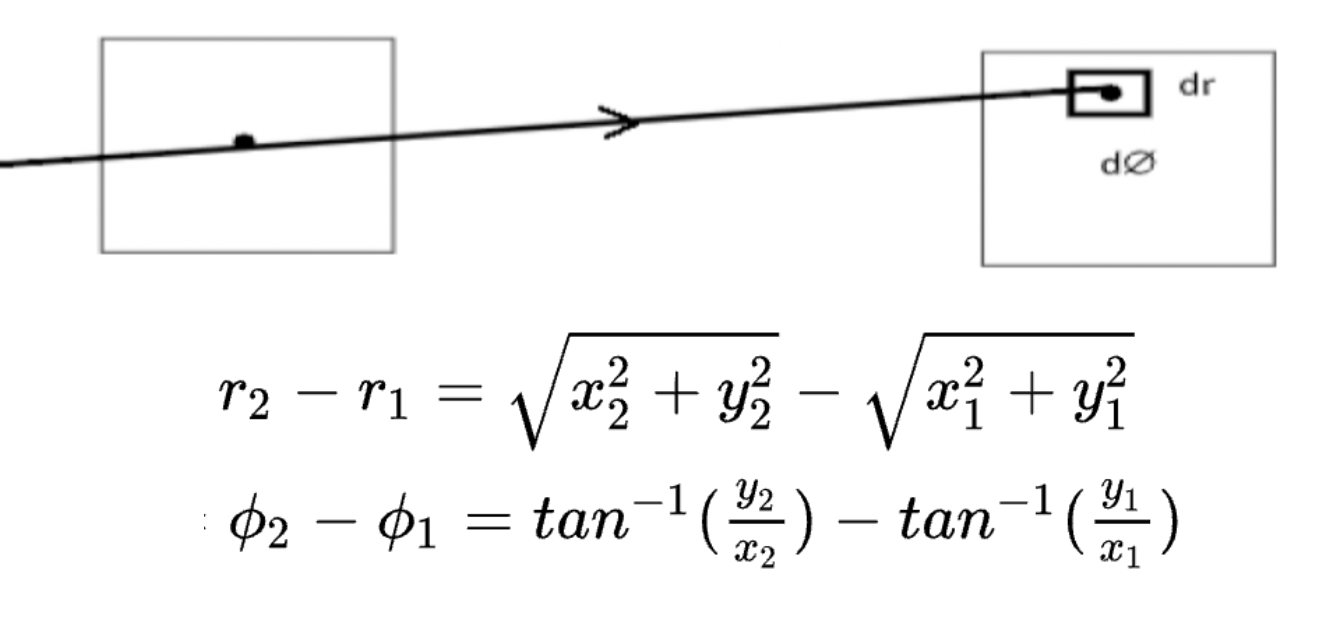
\includegraphics[width=0.7\textwidth]{ashish_thesis/dr_dphi_variables1_1.png}
\caption[New Variables For Two Fold Coincidences]{%
  New r, phi variables used to define coincidence clusters. These variables take into account track angle and curvature.
}
\label{fig:drdphi_diagram}
\end{figure}

\begin{comment}

\begin{figure}[!htp]
\centering
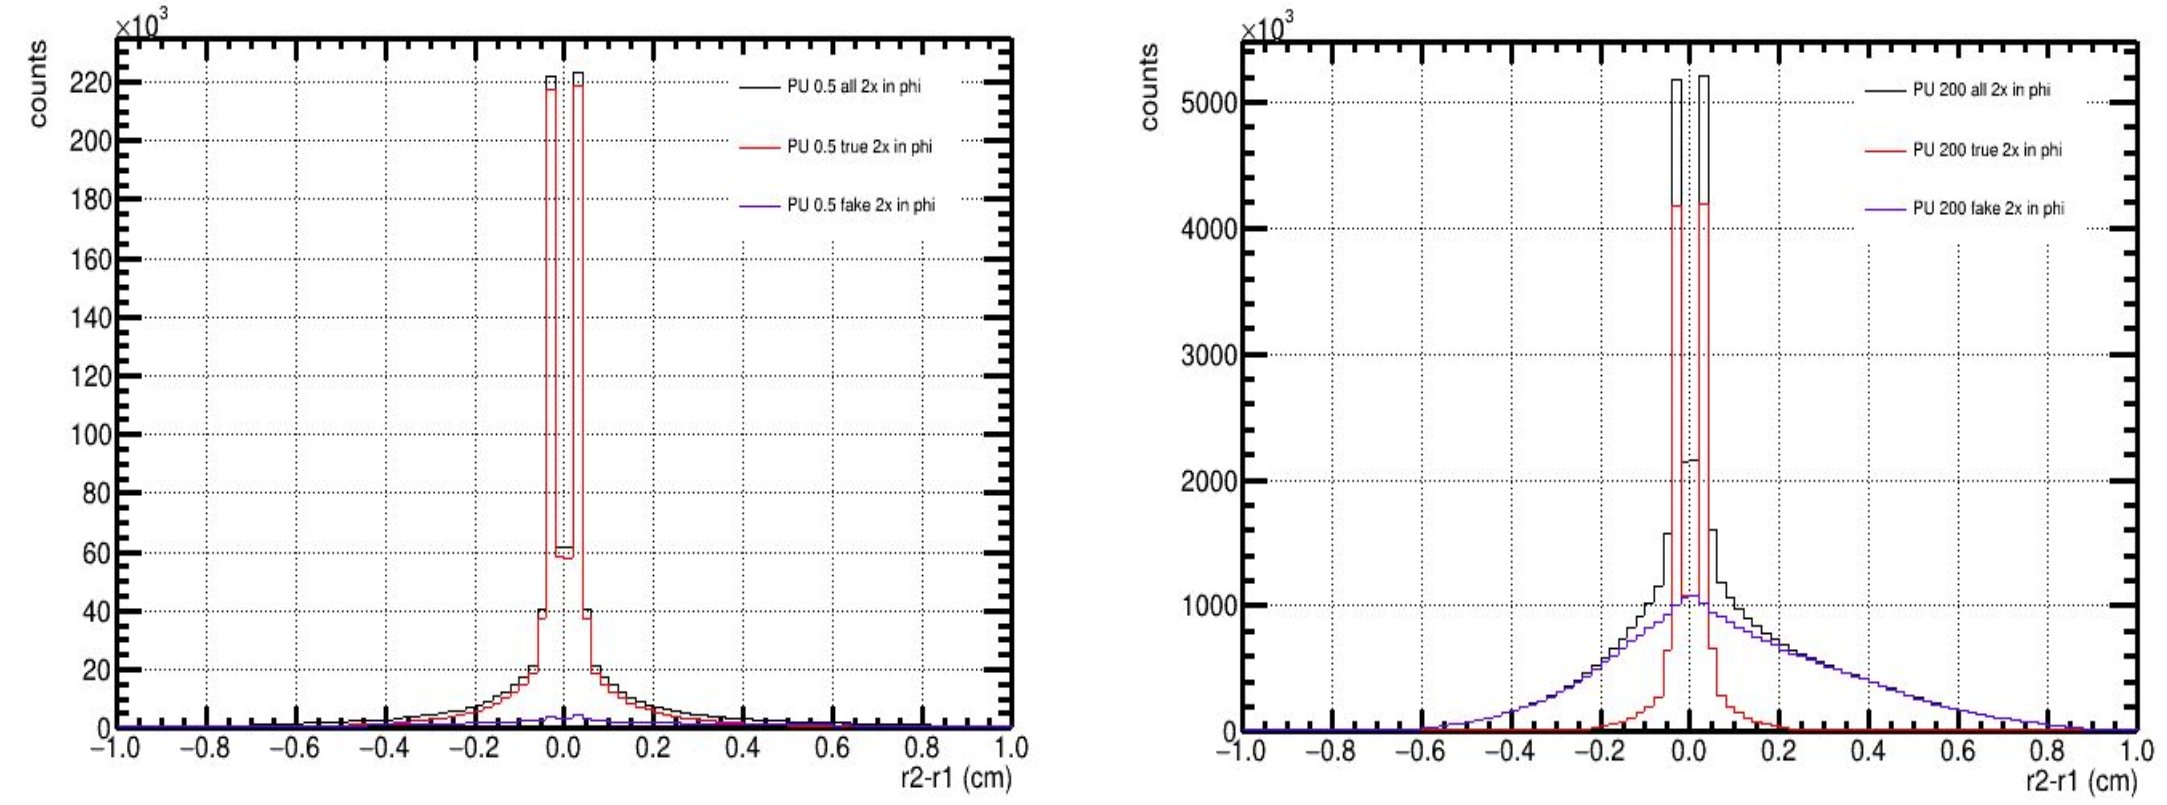
\includegraphics[width=1\textwidth]{ashish_thesis/delta_r.png}
\caption[Total, True & Fake Cluster Counts vs. dr (PU 0.5)]{%
  Distribution of total, true and fake coincidence cluster count as a function of dr variable for pileup 0.5.
}
\label{fig:dr}
\end{figure}

\begin{figure}[!htp]
\centering
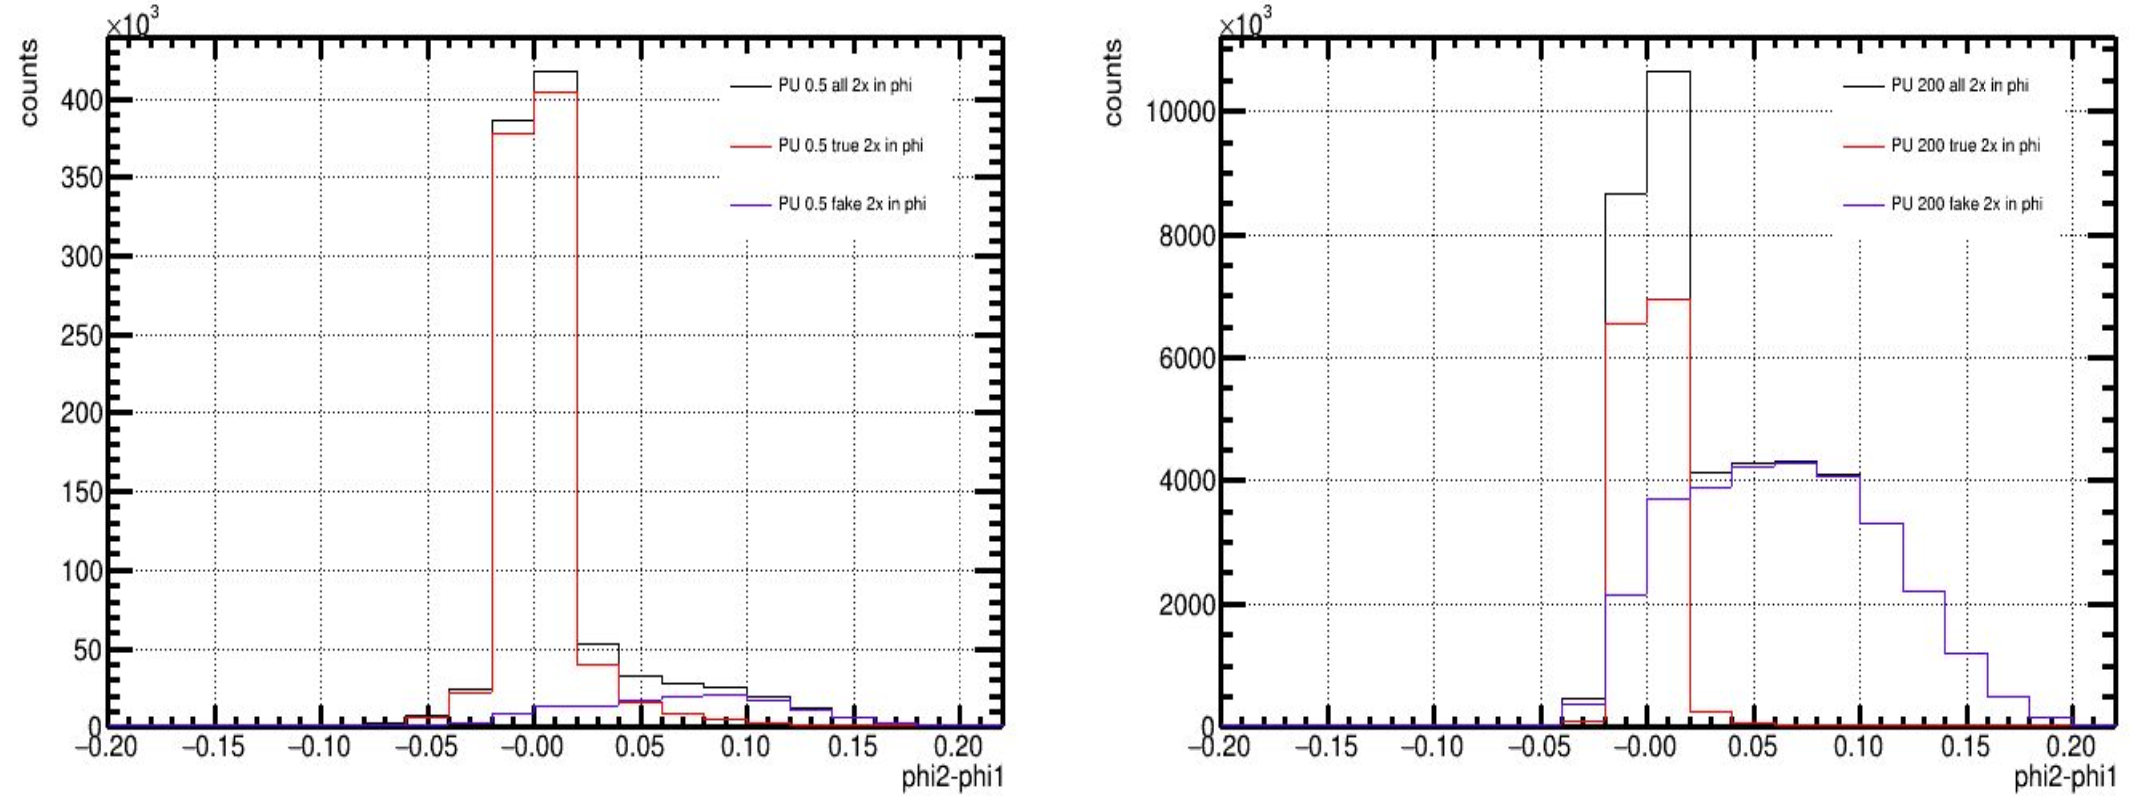
\includegraphics[width=1\textwidth]{ashish_thesis/dphi.png}
\caption[Total, True & Fake Cluster Counts vs. dphi (PU 0.5)]{%
 Distribution of total, true and fake coincidence cluster count as a function of dphi variable for pileup 0.5.
}
\label{fig:dphi}
\end{figure}

\end{comment}

We study the two fold coincidences in phi for all TEPX Disk and rings using dr, dphi variable for pileup 0.5 and apply nominal selection of 0.15 cm on dr and 0.04 on dphi variable in order to remove fake coincidences. After obtaining these distributions for all TEPX disks and rings, we carry out fit of the distribution to obtain mean and standard deviation of these distributions. The dr, dphi distribution showing true, fake, total two fold coincidences for Disk 4 Ring 1 for pileup 0.5 is shown in Fig. \ref{fig:cluster_dr_dphi_dist}.  %Example fits are shown in Fig. \ref{fig:cluster_ring_1003}, \ref{fig:cluster_ring_70}, \ref{fig:cluster_ring_71}. 
While doing the fit, mean value for dphi variable is set to zero. %The mean is taken as the offset value and standard deviation is used as the selection on dr, dphi variables as shown in Table \ref{tab:disk_values}, \ref{tab:mdphi_cuts_values} and \ref{tab:mdr_cuts_offset_values}. 
The mean of the fit is taken as the offset value and standard deviation is used as the selection on dr, dphi variables as shown in Table \ref{tab:disk_values}, \ref{tab:mdphi_cuts_values} and \ref{tab:mdr_cuts_offset_values}.

\begin{figure}[H]
\centering
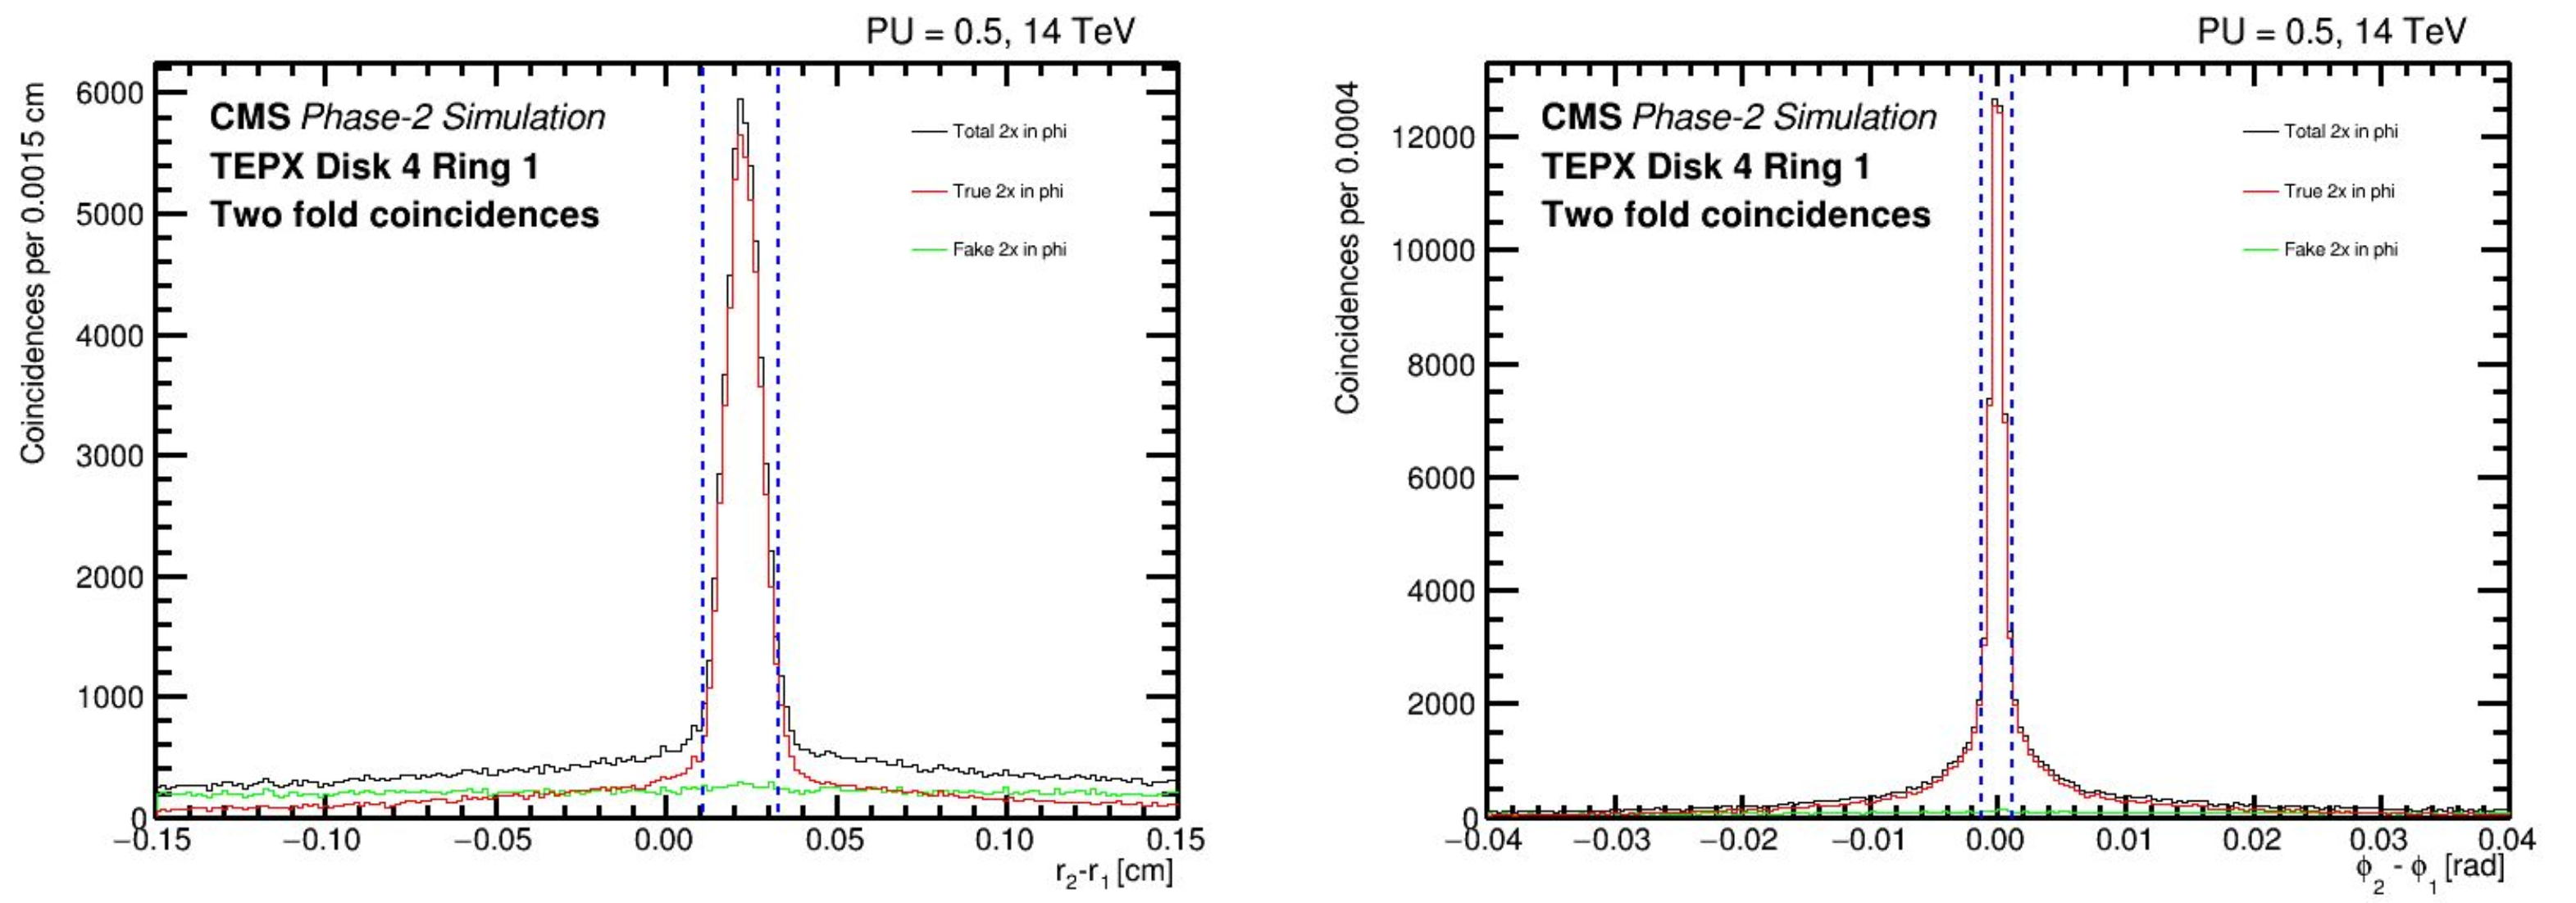
\includegraphics[width=1\textwidth]{ashish_thesis/D4R1_S2_drdphi_cut_1.png}
\caption[Pileup 0.5 Cluster Count in D4R1 (+Z) vs. dr & dphi]{%
  Distribution of cluster count as a function of dr and dphi variables for pileup 0.5 for disk 4 Ring 1 (+Z). Appropriate selection on dr, dphi are used to minimize fake two fold coincidences.
}
\label{fig:cluster_dr_dphi_dist}
\end{figure}


\begin{comment}

\begin{figure}[!htp]
\centering
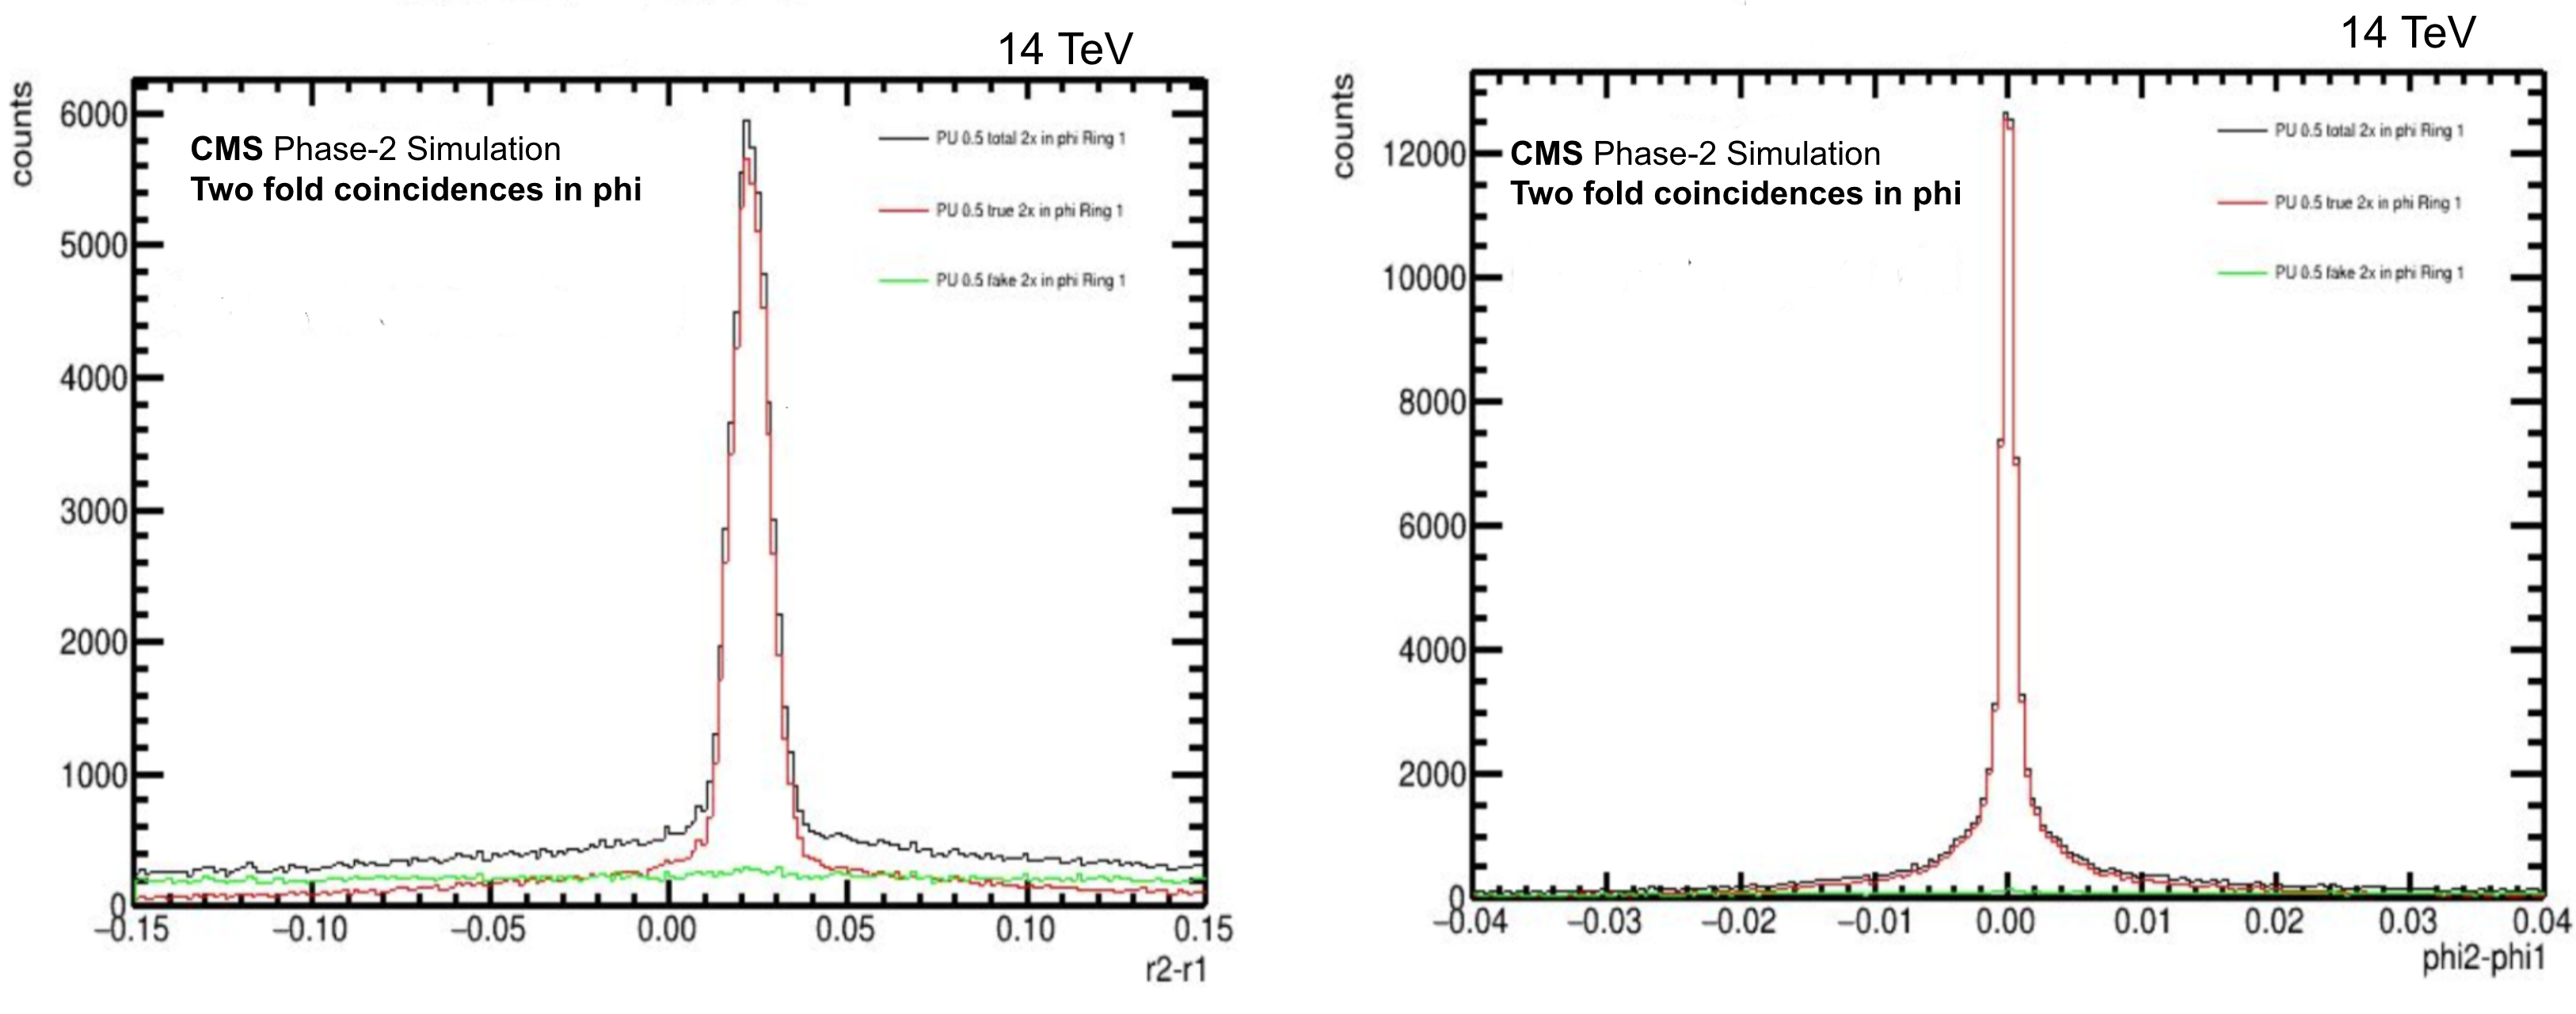
\includegraphics[width=1\textwidth]{ashish_thesis/D4R1_S2_drdphi_cut.png}
\caption[Pileup 0.5 Cluster Count in D4R1 (+Z) vs. dr & dphi]{%
  Distribution of cluster count as a function of dr and dphi variables for pileup 0.5 for disk 4 Ring 1 (+Z). Appropriate selection on dr, dphi are used to minimize fake two fold coincidences.
}
\label{fig:cluster_dr_dphi_dist}
\end{figure}


\begin{figure}[!htp]
\centering
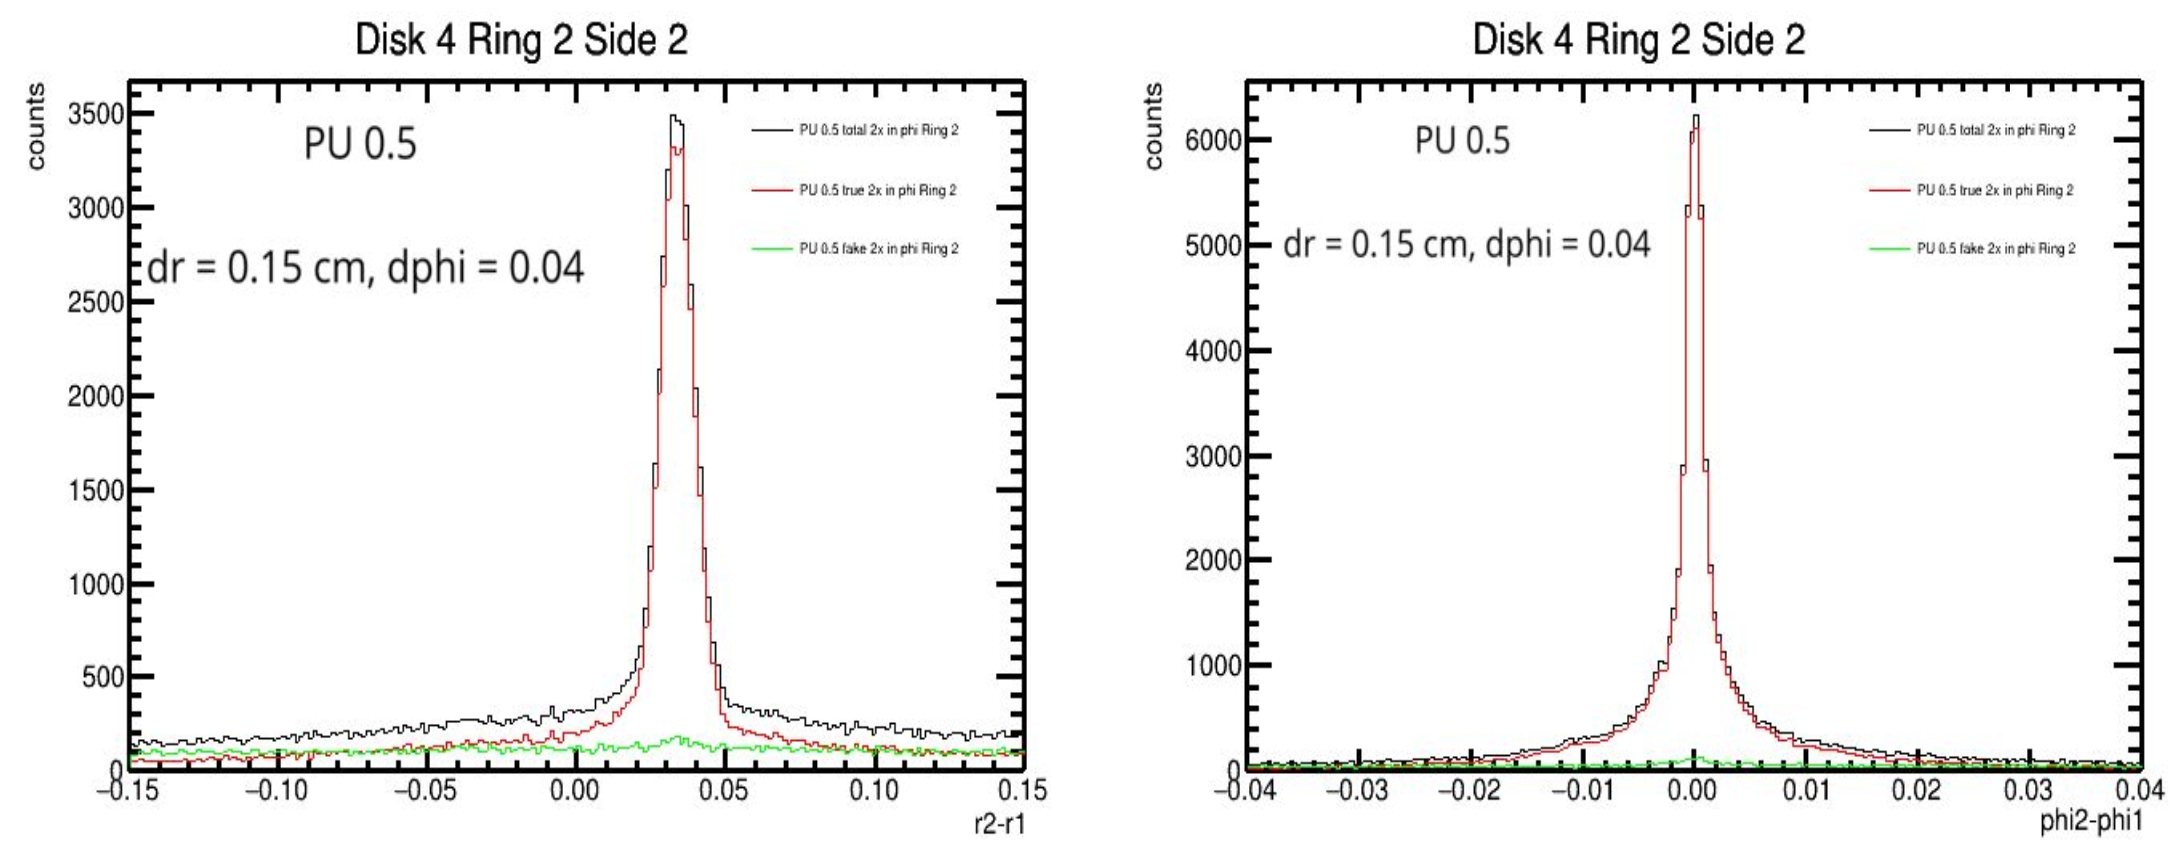
\includegraphics[width=1\textwidth]{ashish_thesis/D4R2_S2_drdphicut.png}
\caption[Pileup 0.5 Cluster Count in D4R2 (+Z) vs. dr & dphi]{%
   Distribution of cluster count as a function of dr and dphi variables for pileup 0.5 for disk 4 Ring 2 (+Z). Appropriate selection on dr, dphi are used to minimize fake two fold coincidences.
}
\label{fig:cluster_ring_1000}
\end{figure}


\begin{figure}[!htp]
\centering
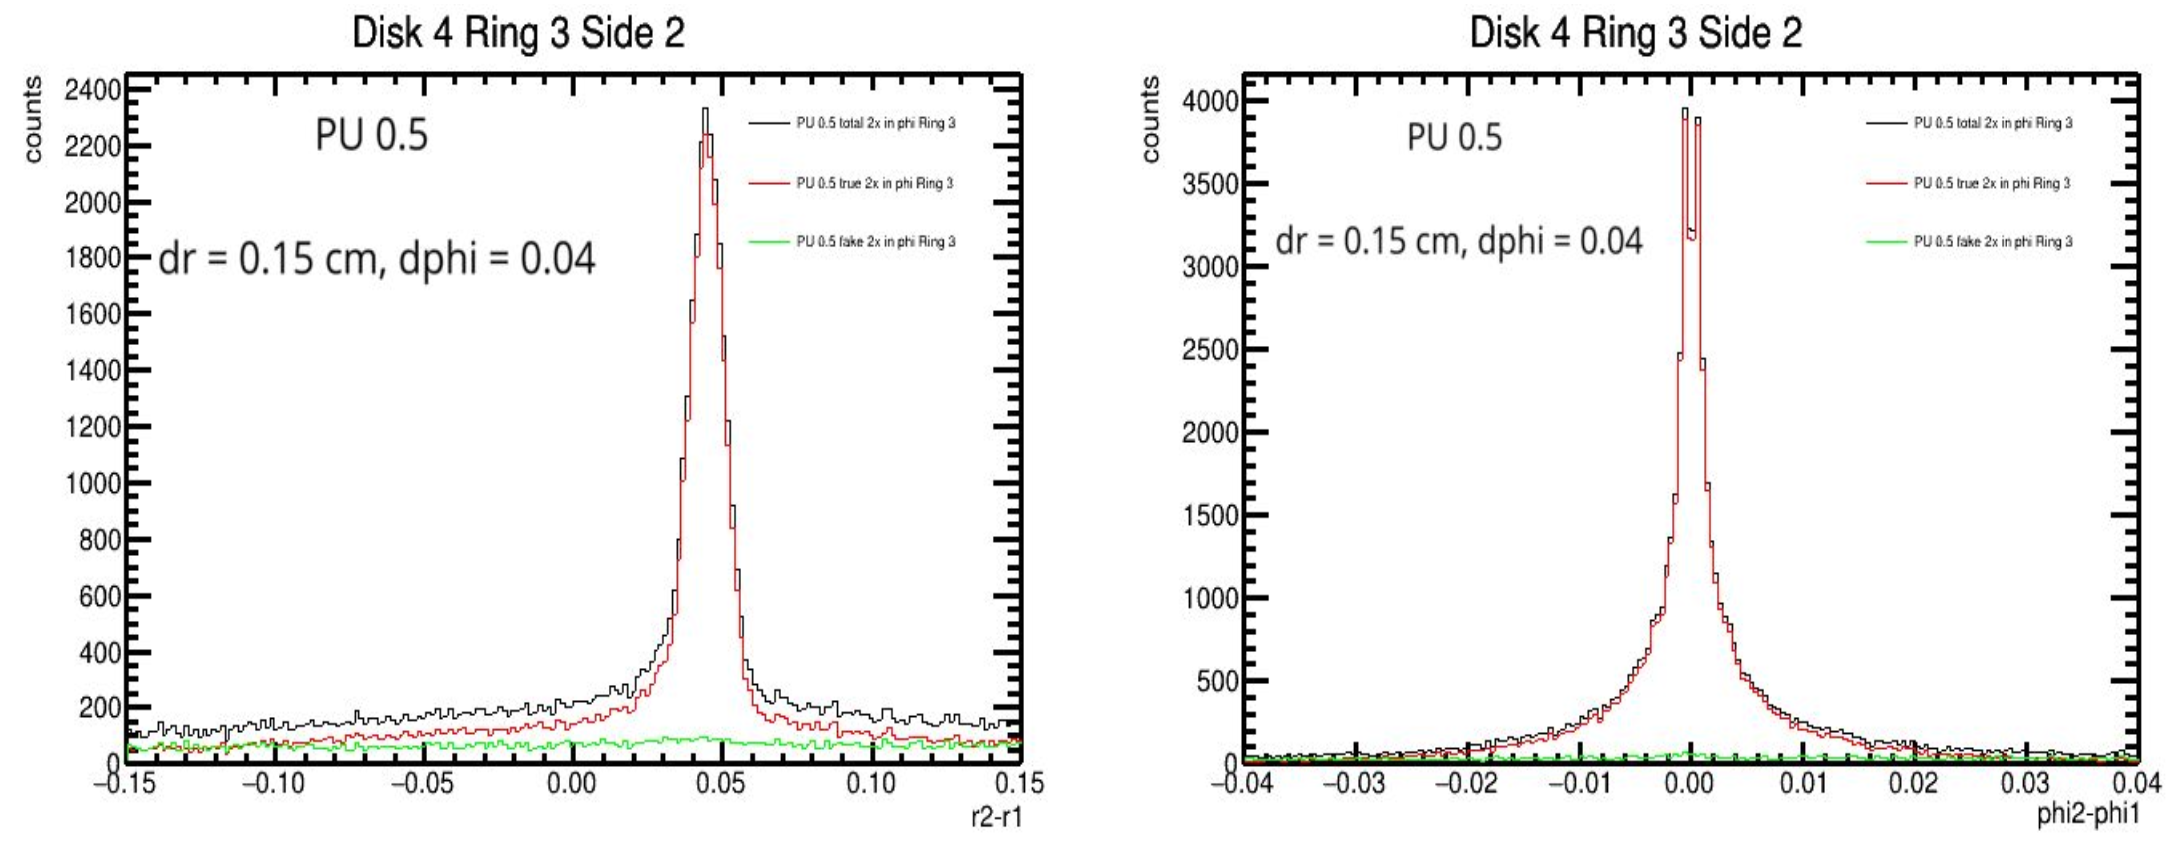
\includegraphics[width=1\textwidth]{ashish_thesis/D4R3_S2_drdphi_cut.png}
\caption[Pileup 0.5 Cluster Count in D4R3 (+Z) vs. dr & dphi]{%
  Distribution of cluster count as a function of dr and dphi variables for pileup 0.5 for disk 4 Ring 3 (+Z). Appropriate selection on dr, dphi are used to minimize fake two fold coincidences.
}
\label{fig:cluster_ring_10001}
\end{figure}


\begin{figure}[!htp]
\centering
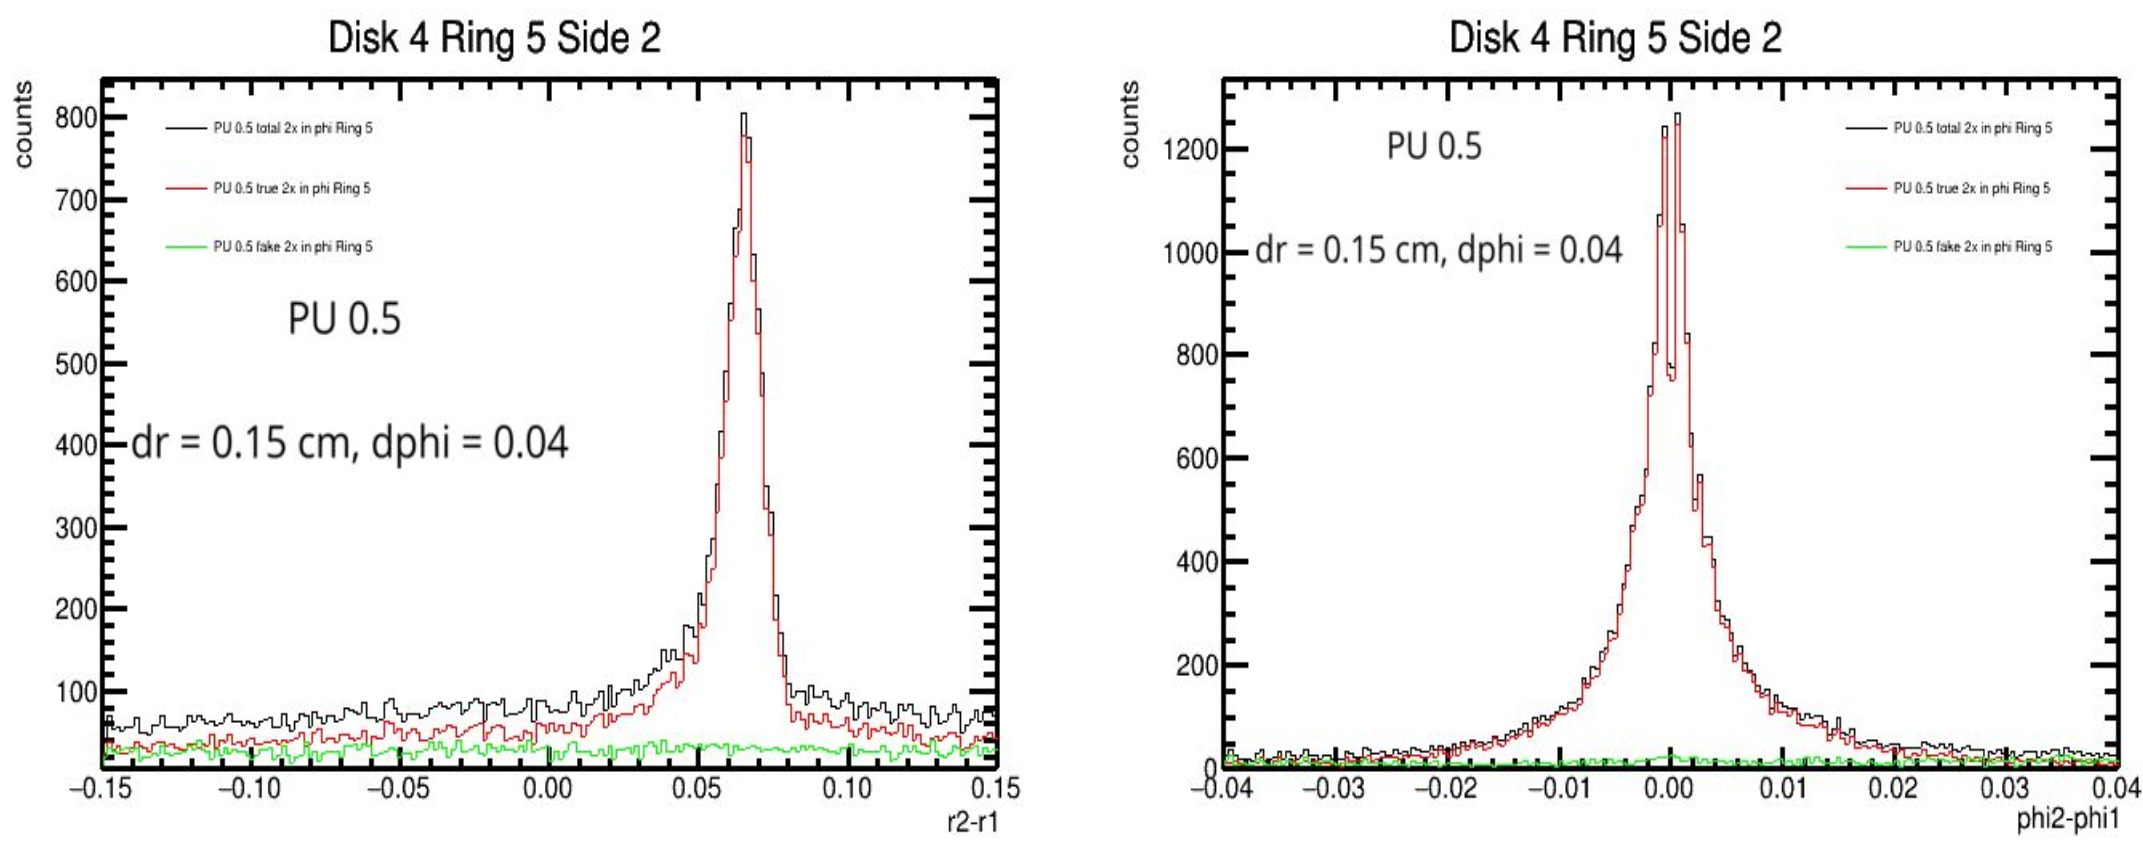
\includegraphics[width=1\textwidth]{ashish_thesis/D4R5_drdphicut.png}
\caption[Pileup 0.5 Cluster Count in D4R5 (+Z) vs. dr & dphi]{%
  Distribution of cluster count as a function of dr and dphi variables for pileup 0.5 for disk 4 Ring 5 (+Z). Appropriate selection on dr, dphi are used to minimize fake two fold coincidences.
}
\label{fig:cluster_ring_1002}
\end{figure}


\begin{figure}[!htp]
\centering
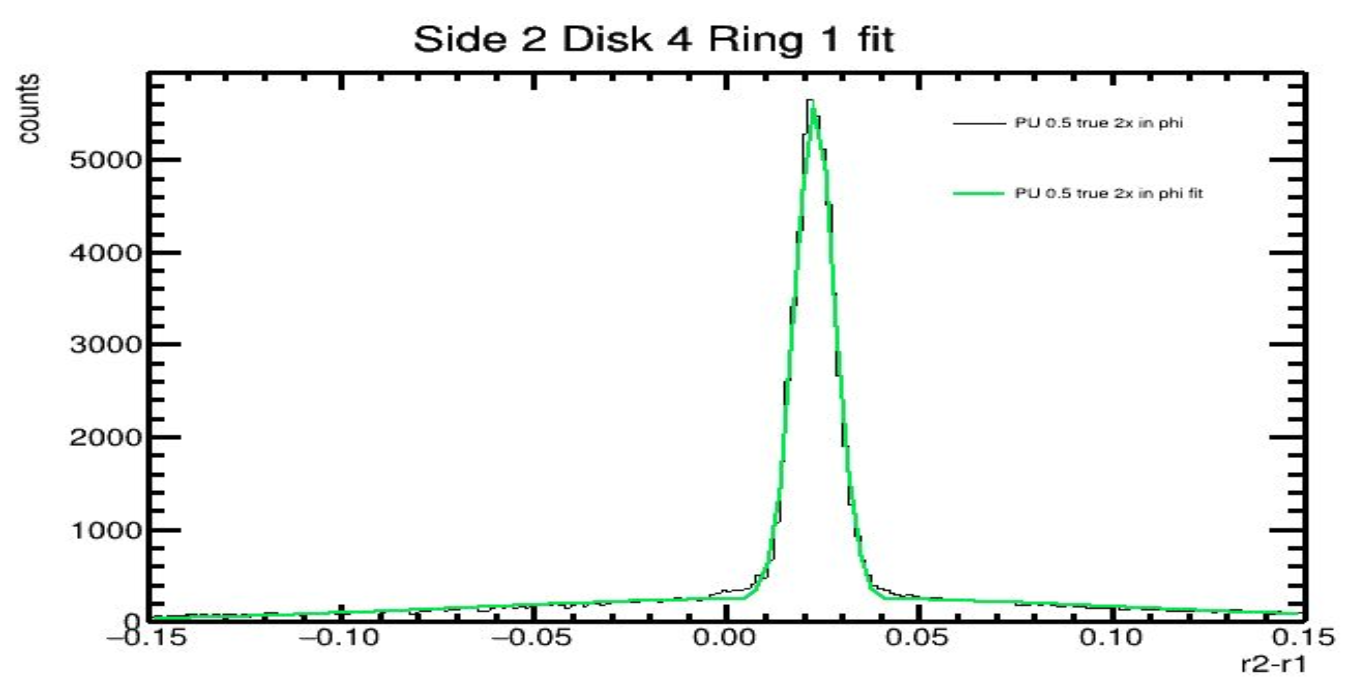
\includegraphics[width=1\textwidth]{ashish_thesis/D4R1S2_fit.png}
\caption[Disk 4 Ring 1 Clusters Fit]{%
   Example fit using single gaussian function of cluster count as a function of dr variable for Disk 4 Ring 1 (+Z).
}
\label{fig:cluster_ring_1003}
\end{figure}


\begin{comment}
  
\begin{figure}[!htp]
\centering
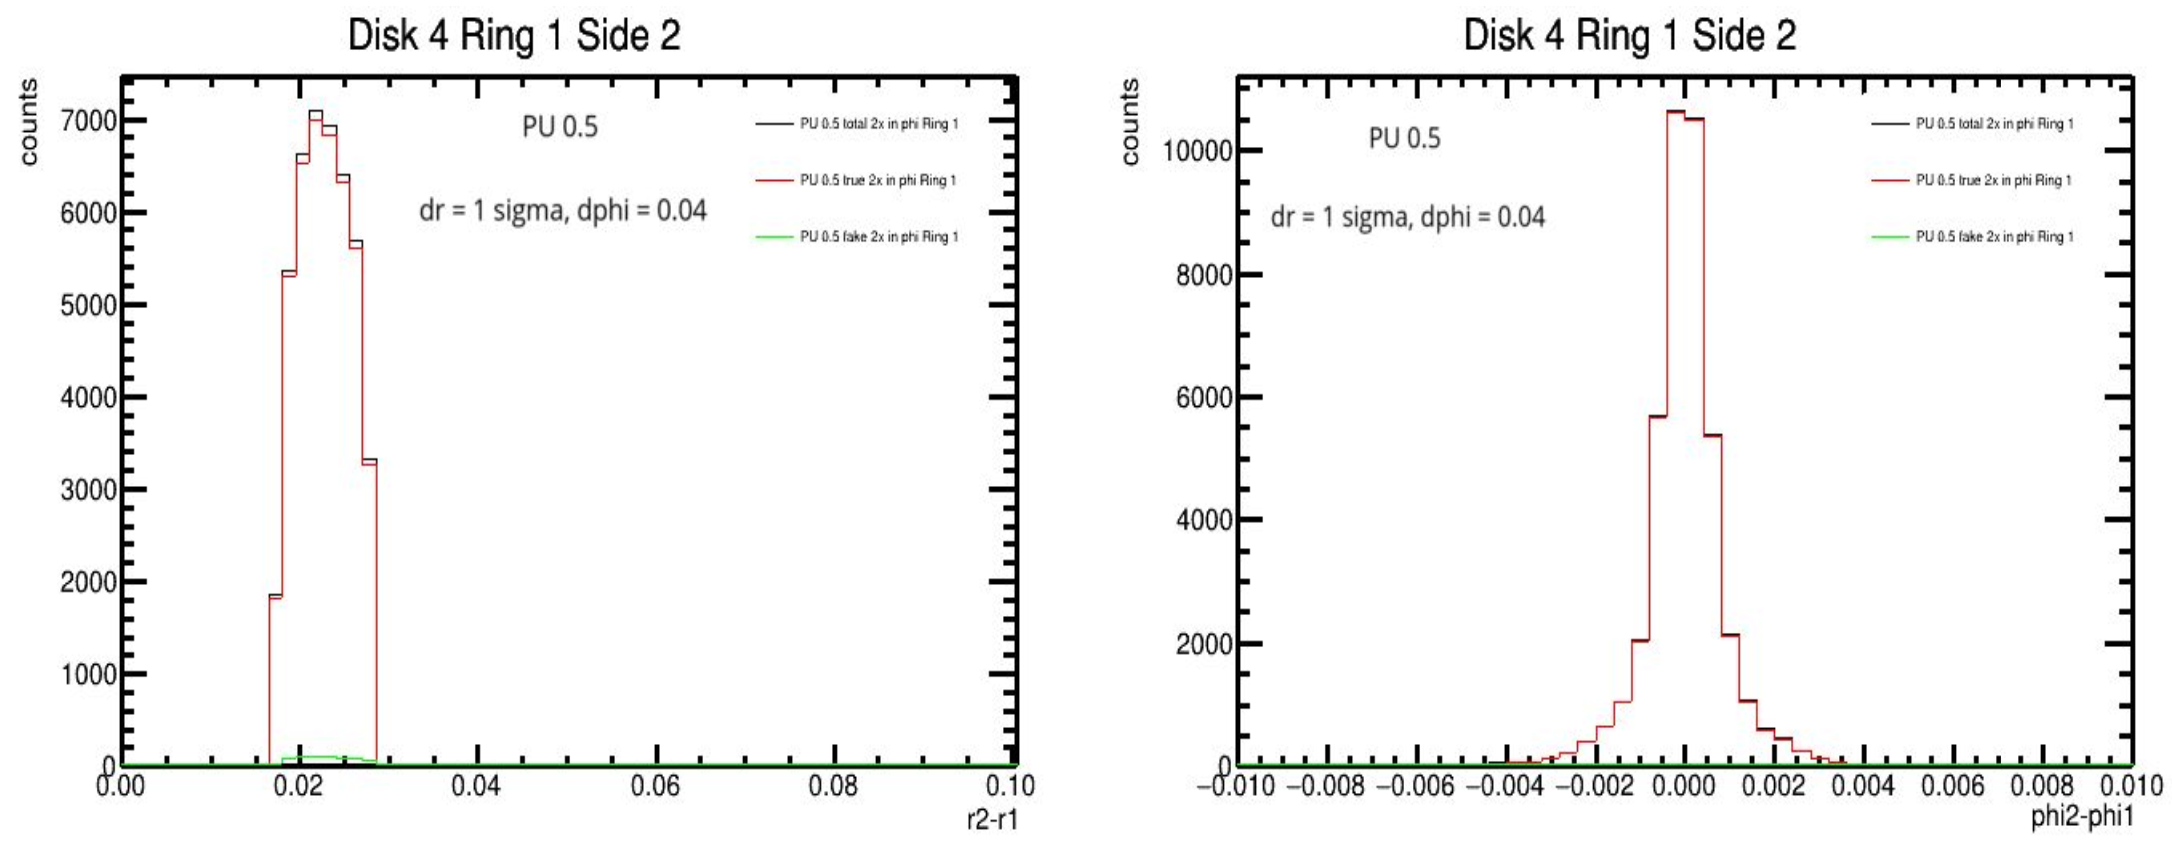
\includegraphics[width=1\textwidth]{ashish_thesis/D4R1S2_dr_dphi_cut.png}
\caption[New dr selection value]{%
 Distribution of cluster count as a function of dr and dphi variables for pileup 0.5 for disk 4 Ring 1 (+Z). 1 sigma selection on dr and dphi equal to 0.04 are used to minimize fake two fold coincidence.
}
\label{fig:cluster_ring_1004}
\end{figure}

\begin{figure}[!htp]
\centering
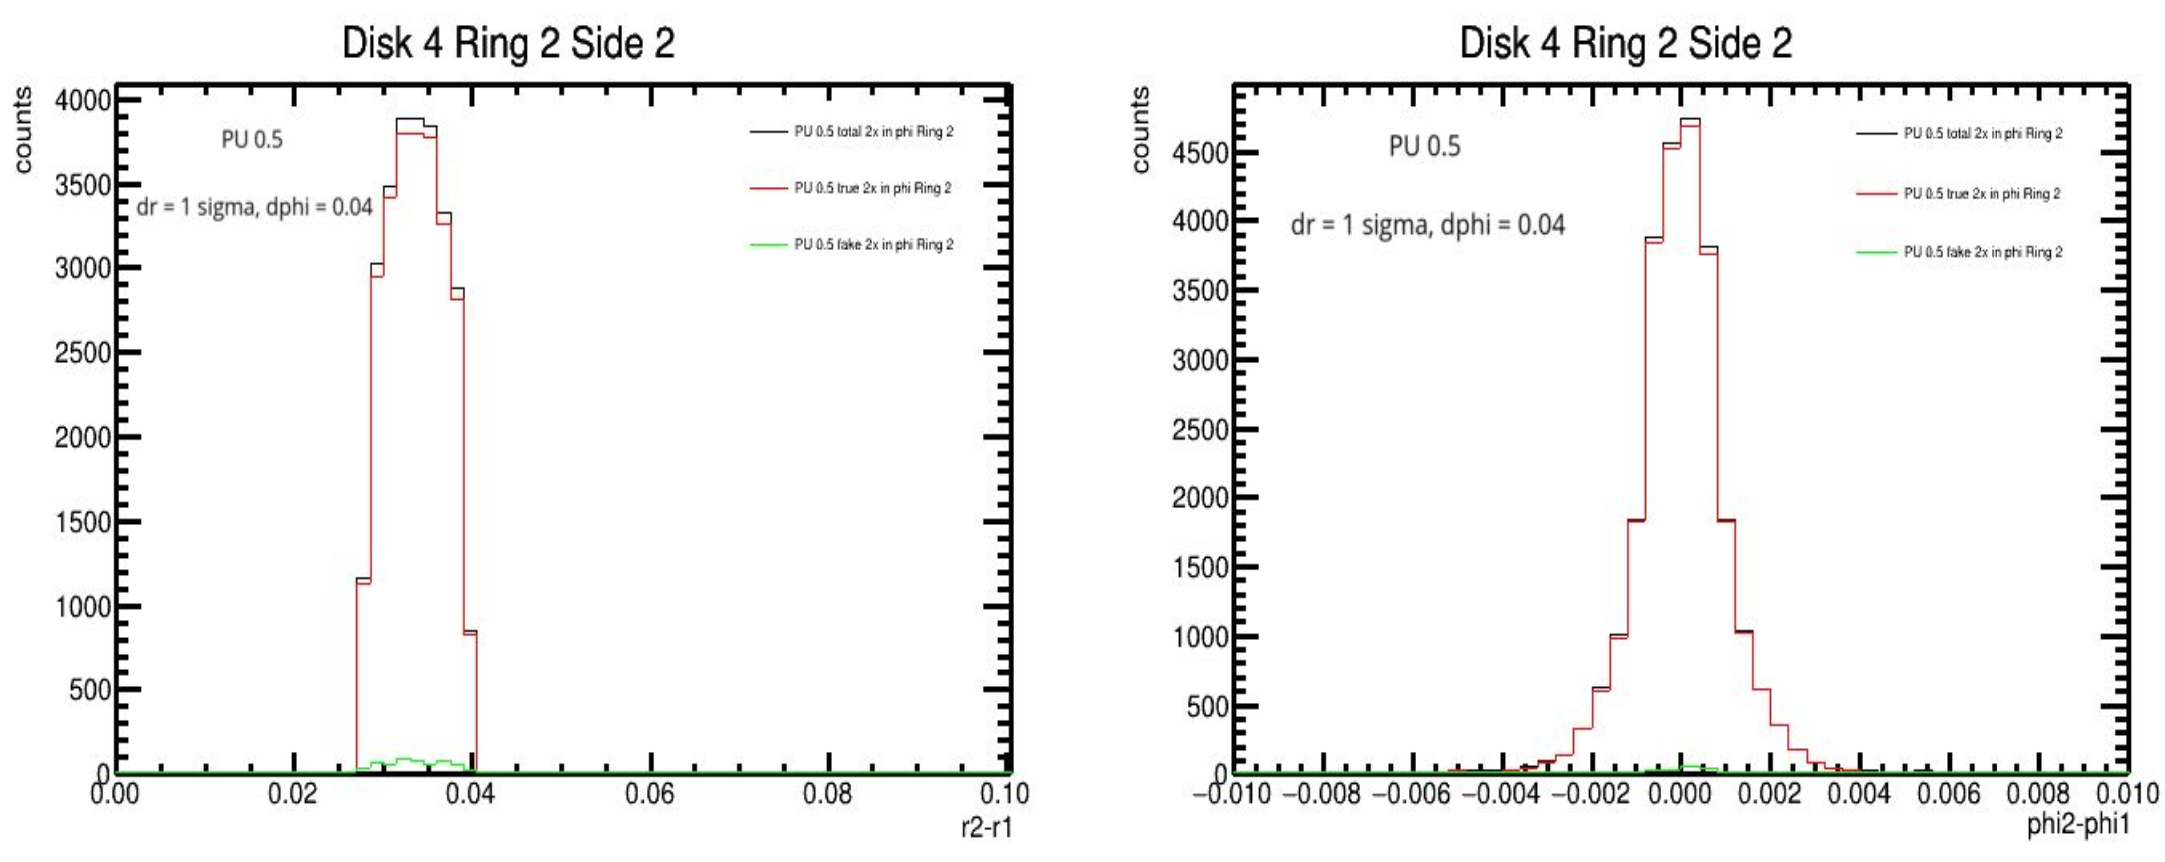
\includegraphics[width=1\textwidth]{ashish_thesis/D4R2S2_dr_dphi_cut.png}
\caption[New dphi selection value]{%
   Distribution of cluster count as a function of dr and dphi variables for pileup 0.5 for disk 4 Ring 2 (+Z). 1 sigma selection on dr and dphi equal to 0.04 are used to minimize fake two fold coincidences.
}
\label{fig:cluster_ring_1005}
\end{figure}


\begin{figure}[!htp]
\centering
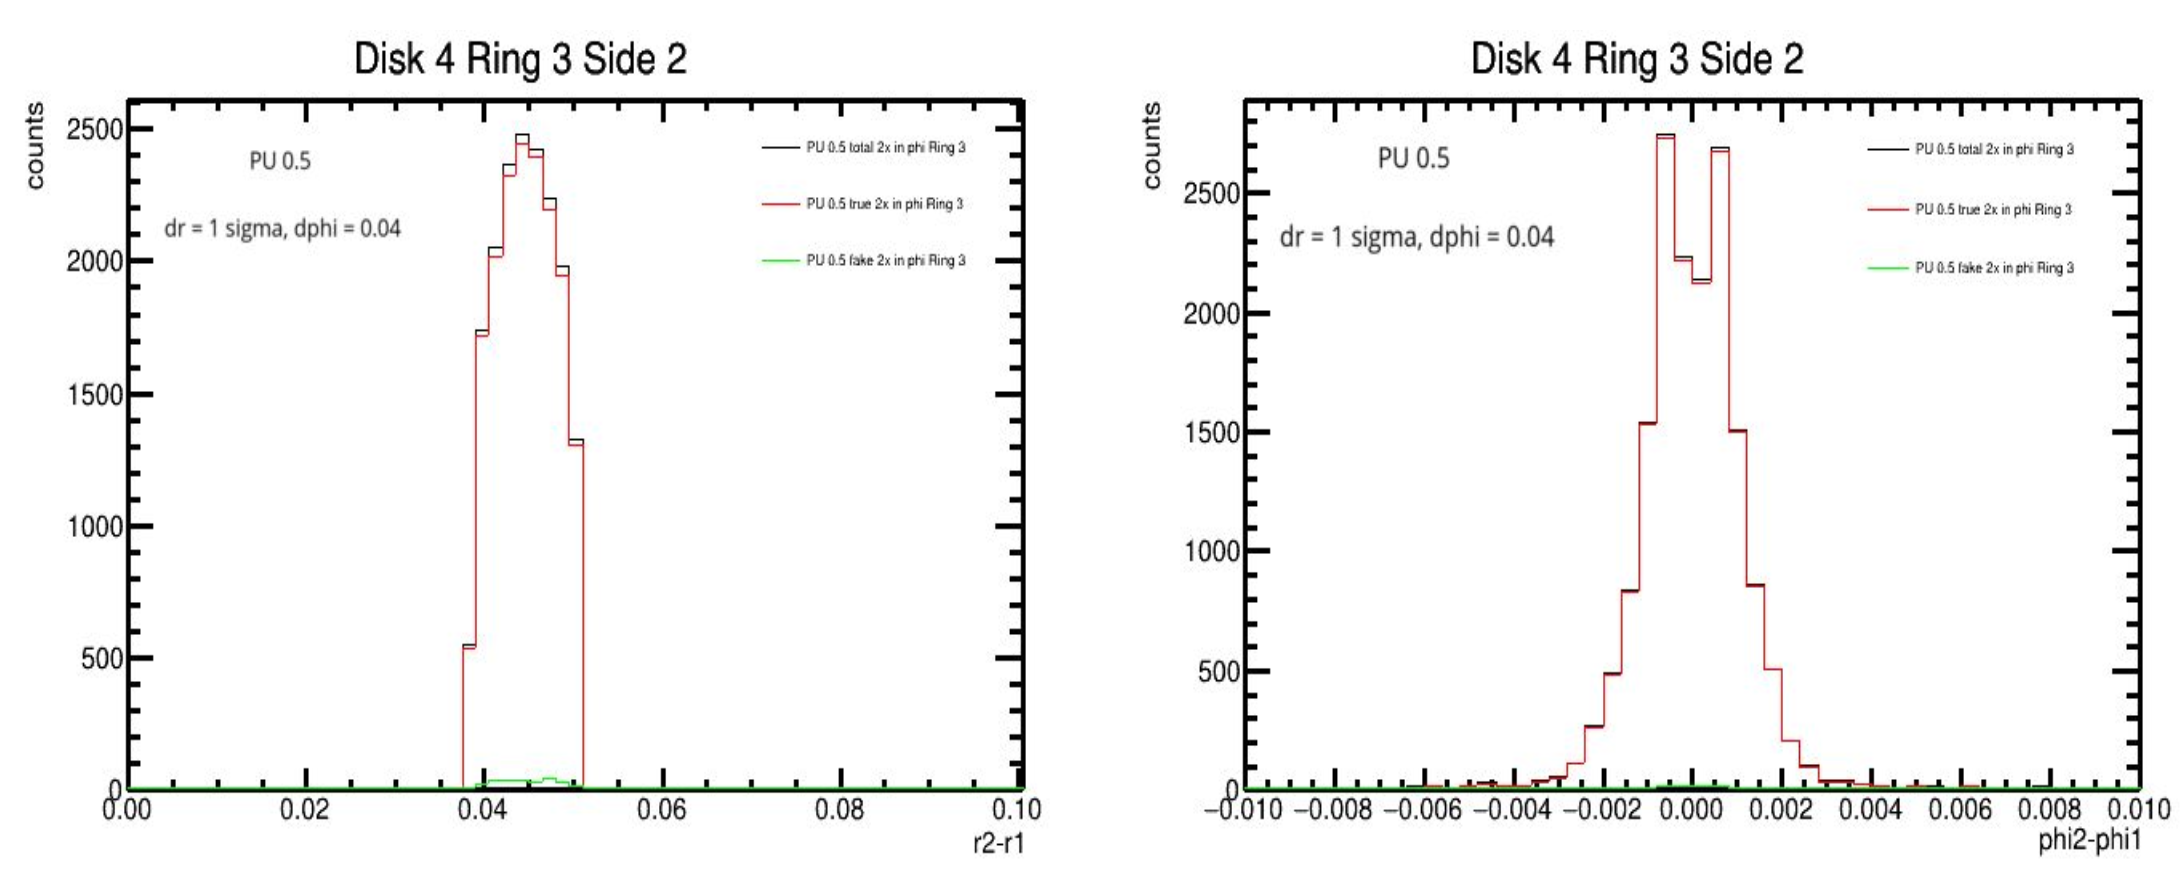
\includegraphics[width=1\textwidth]{ashish_thesis/D4R3S2_dr_dphi_cut.png}
\caption[Cluster count as function of new variables with selection for PU 0.5 D4R3S2]{%
    Distribution of cluster count as a function of dr and dphi variables for pileup 0.5 for disk 4 Ring 3 (+Z). 1 sigma selection on dr and dphi equal to 0.04 are used to minimize fake two fold coincidences.
}
\label{fig:cluster_ring_1006}
\end{figure}


\begin{figure}[!htp]
\centering
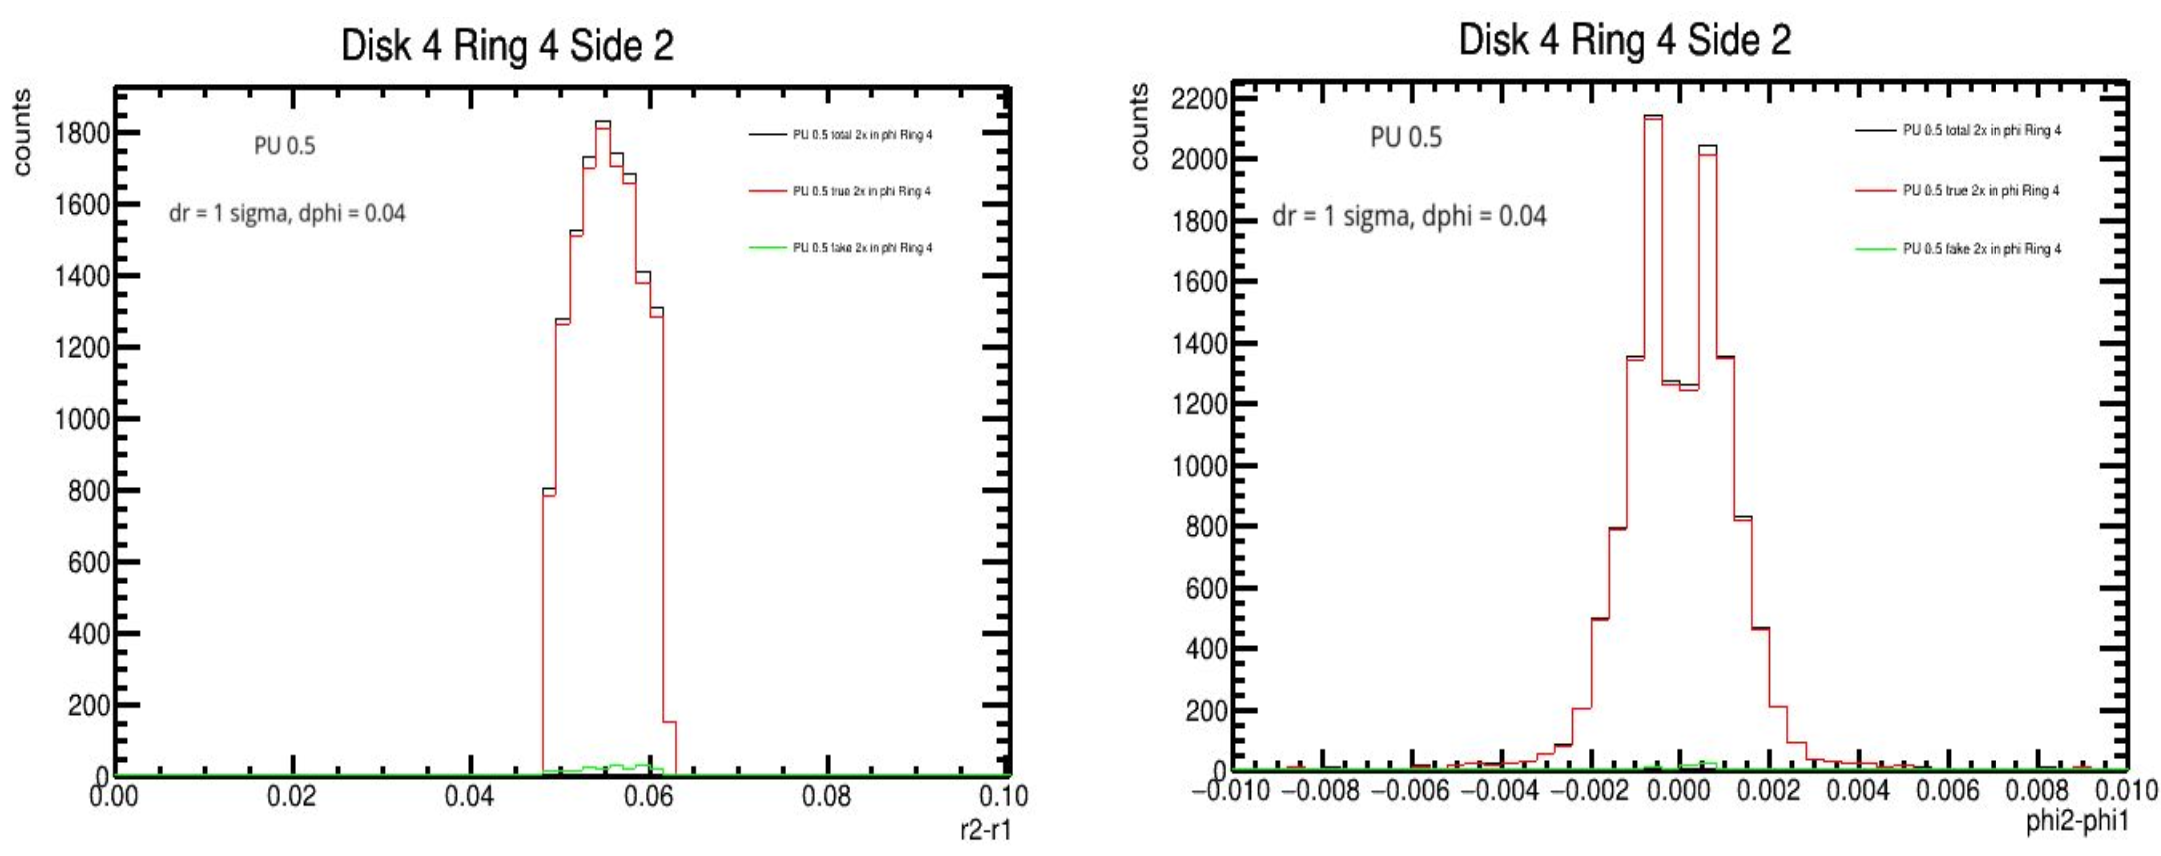
\includegraphics[width=1\textwidth]{ashish_thesis/D4R4S2_dr_dphi_cut.png}
\caption[Cluster count as function of new variables with selection for PU 0.5 D4R4S2]{%
  Distribution of cluster count as a function of dr and dphi variables for pileup 0.5 for disk 4 Ring 4 (+Z). 1 sigma selection on dr and dphi equal to 0.04 are used to minimize fake two fold coincidences.  
}
\label{fig:cluster_ring_68}
\end{figure}


\begin{figure}[!htp]
\centering
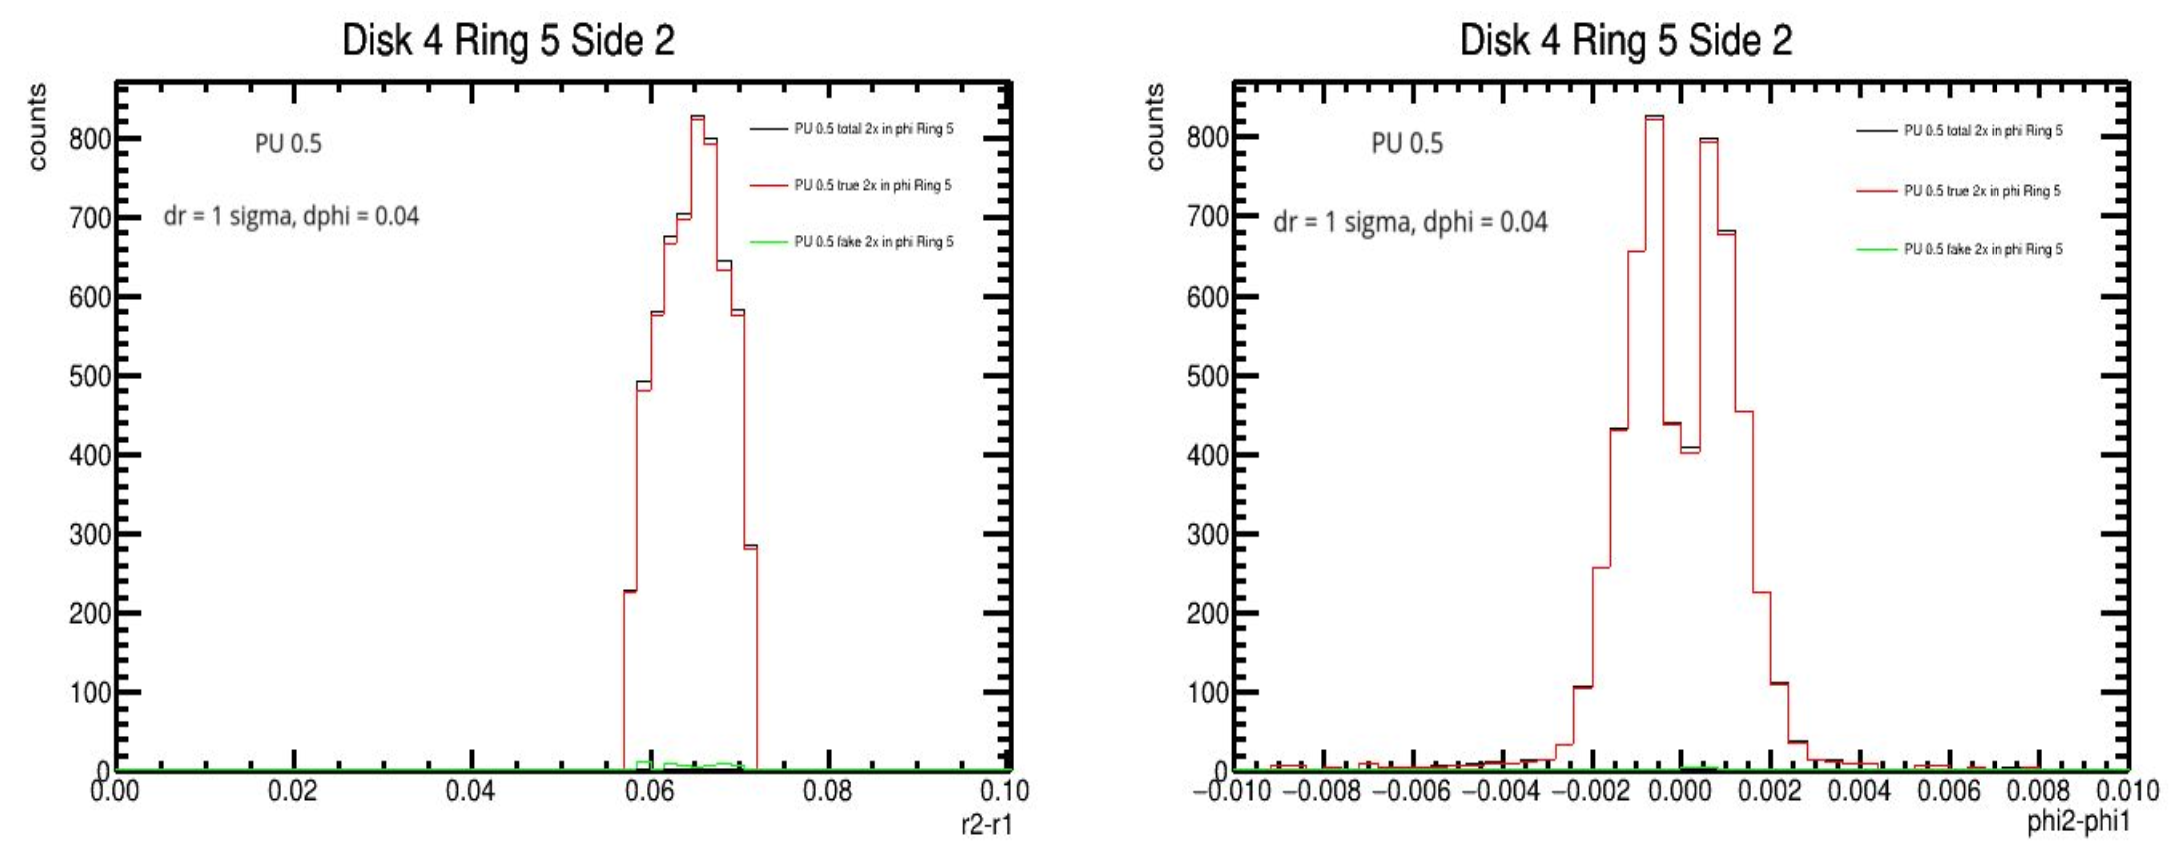
\includegraphics[width=1\textwidth]{ashish_thesis/D4R5S2_dr_dphi_cut.png}
\caption[Cluster count as function of new variables with selection for PU 0.5 D4R5S2]{%
  Distribution of cluster count as a function of dr and dphi variables for pileup 0.5 for disk 4 Ring 5 (+Z). 1 sigma selection on dr and dphi equal to 0.04 are used to minimize fake two fold coincidence clusters.  
}
\label{fig:cluster_ring_69}
\end{figure}

%\end{comment}


\begin{figure}[!htp]
\centering
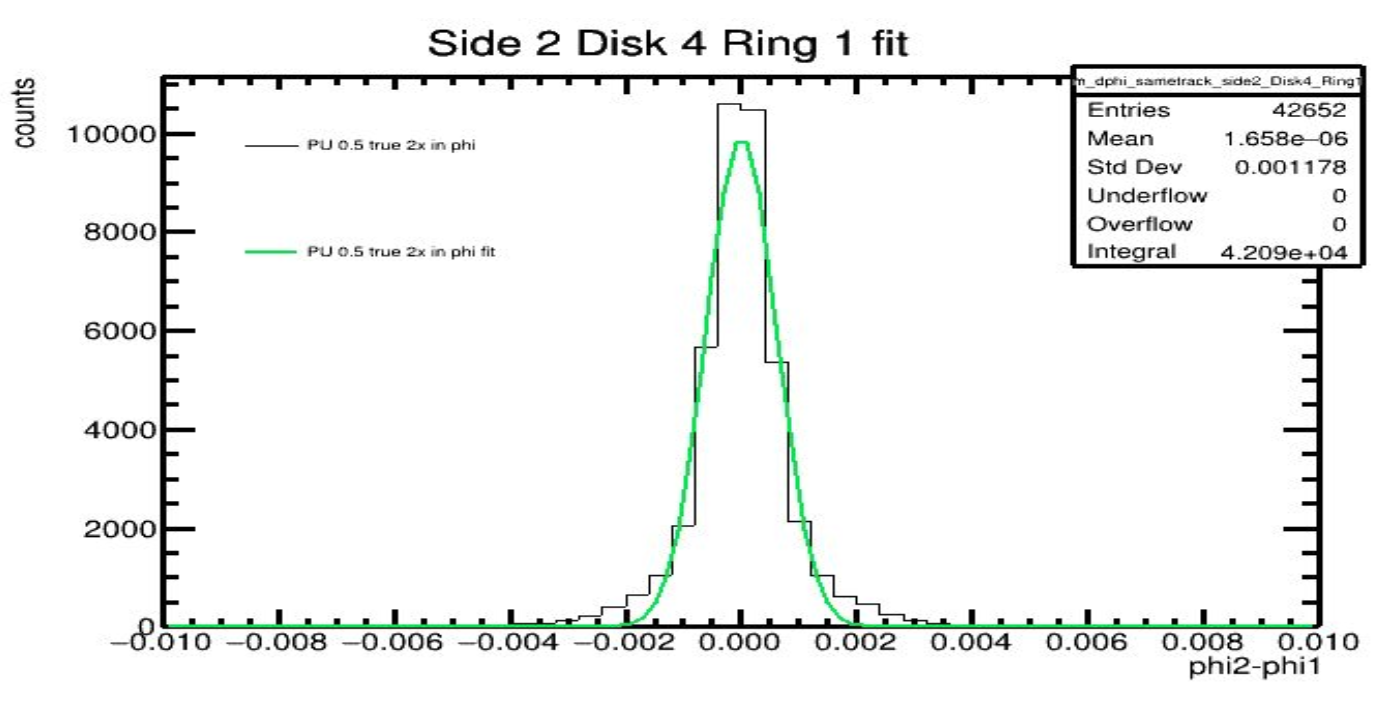
\includegraphics[width=1\textwidth]{ashish_thesis/D4R1S2_fit_PU0p5.png}
\caption[Fit Disk 4 Ring 1 (+Z) Cluster Distribution]{%
  Example fit using single Gaussian function of cluster count as a function of dphi variable for pileup 0.5 Disk 4 Ring 1 (+Z).
}
\label{fig:cluster_ring_70}
\end{figure}


\begin{figure}[!htp]
\centering
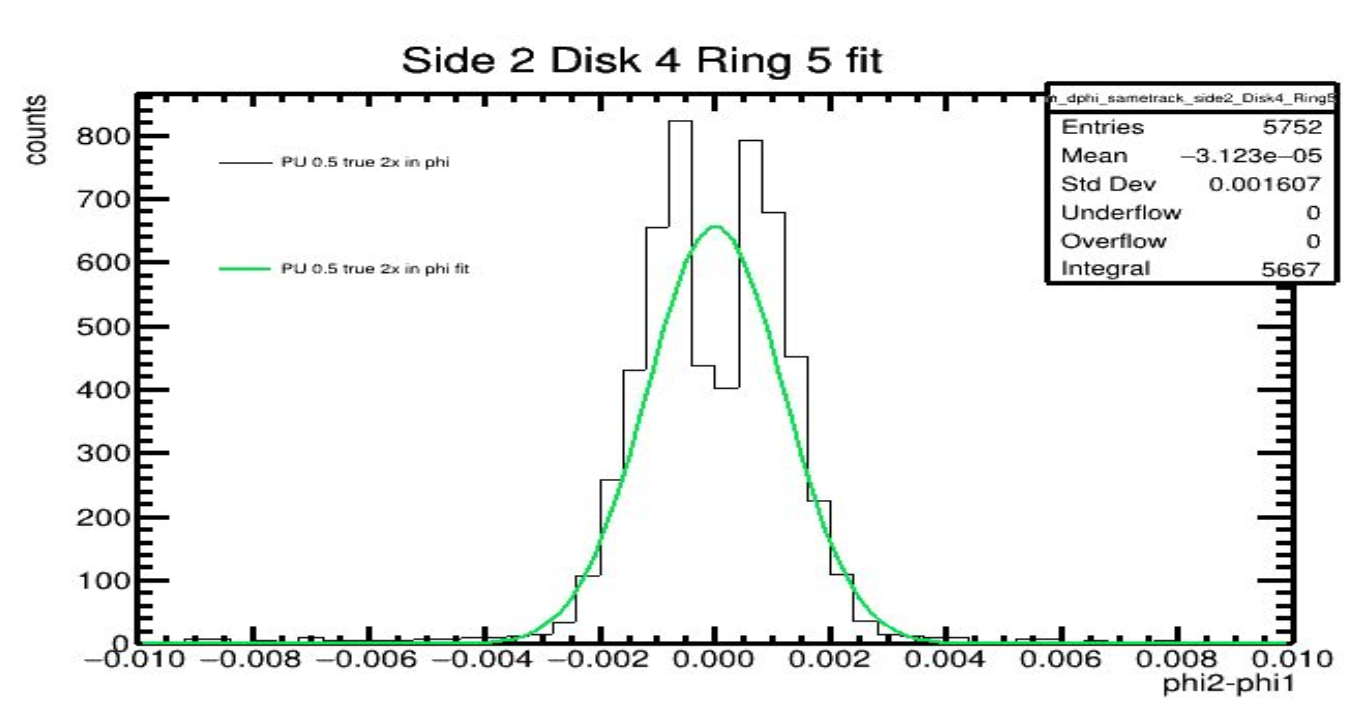
\includegraphics[width=1\textwidth]{ashish_thesis/D4R5_fit_PU0p5.png}
\caption[Fit Disk 4 Ring 5 (+Z) Cluster Distribution]{%
 Example fit using single Gaussian function of cluster count as a function of dphi variable for pileup 0.5 Disk 4 Ring 5 (+Z). 
}
\label{fig:cluster_ring_71}
\end{figure}

\end{comment}


%The mean of the fit is taken as the offset value and standard deviation is used as the selection on dr, dphi variables as shown in Table \ref{tab:disk_values}, \ref{tab:mdphi_cuts_values} and \ref{tab:mdr_cuts_offset_values}.

\begin{table}[h]
  \centering
  \caption[dr cut values]{dr cut values for two fold coincidences in phi for all disks and rings}
  \begin{tabular}{cccccc}
    \textbf{Disk} & \textbf{Ring 1} & \textbf{Ring 2} & \textbf{Ring 3} & \textbf{Ring 4} & \textbf{Ring 5} \\
    \hline
    %-1 & 0.00633554 & 0.00709231 & 0.00757662 & 0.008659   & 0.00872148 \\
    %-2 & 0.00594206 & 0.00663493 & 0.00718173 & 0.00766371 & 0.00797059 \\
    %-3 & 0.00594206 & 0.00663493 & 0.00660603 & 0.00713035 & 0.00679445 \\
    %-4 & 0.00530235 & 0.00587692 & 0.00616465 & 0.00661972 & 0.00660599 \\
    1  & 0.0064 & 0.0072  & 0.0078 & 0.0086 & 0.0088 \\
    2  & 0.0059 & 0.0066 & 0.0070 & 0.0077 & 0.0079 \\
    3  & 0.0056 & 0.0062 & 0.0066 & 0.0070  & 0.0073 \\
    4  & 0.0053  & 0.0059 & 0.0061  & 0.0067 & 0.0068 \\
  \end{tabular}
  \label{tab:disk_values}
\end{table}



\begin{table}[h]
  \centering
  \caption[dphi cut values]{dphi cut values for two fold coincidences in phi for all disks and rings}
  \begin{tabular}{cccccc}
    \textbf{Disk} & \textbf{Ring 1} & \textbf{Ring 2} & \textbf{Ring 3} & \textbf{Ring 4} & \textbf{Ring 5} \\
    \hline
    %-1 & 0.000856727  & 0.00128078   & 0.00151297   & 0.00151297   & 0.0016561    \\
    %-2 & 0.000765842  & 0.00110698   & 0.00131104   & 0.00143555   & 0.00150265   \\
    %-3 & 0.000684645  & 0.000975385  & 0.00115899   & 0.00126858   & 0.00131598   \\
    %-4 & 0.000598839  & 0.000862728  & 0.00104327   & 0.00112621   & 0.00115609   \\
    1  & 0.00088  & 0.0013   & 0.0015    & 0.0016   & 0.0017   \\
    2  & 0.00076   & 0.0011   & 0.0013   & 0.0014   & 0.0015   \\
    3  & 0.00068  & 0.00097  & 0.0012   & 0.0013   & 0.0013   \\
    4  & 0.00061  & 0.00088  & 0.0010   & 0.0011   & 0.0012   \\
  \end{tabular}
  \label{tab:mdphi_cuts_values}
\end{table}



\begin{table}[h]
  \centering
  \caption[dr offset values]{dr mean values obtained from fit for two fold coincidences in phi for all disks and rings}
  \begin{tabular}{cccccc}
    \textbf{Disk} & \textbf{Ring 1} & \textbf{Ring 2} & \textbf{Ring 3} & \textbf{Ring 4} & \textbf{Ring 5} \\
    \hline
    %-1 & 0.0342041  & 0.0511416 & 0.0676943 & 0.0834355 & 0.0984932 \\
    %-2 & 0.0298276  & 0.0445398 & 0.0589828 & 0.0727454 & 0.0853587 \\
    %-3 & 0.0260326  & 0.0386608 & 0.05122   & 0.0632478 & 0.0746467 \\
    %-4 & 0.0227089  & 0.0336467 & 0.044476  & 0.0551065 & 0.06484   \\
    1  & 0.034  & 0.051 & 0.068 & 0.084 & 0.098 \\
    2  & 0.030  & 0.044 & 0.059 & 0.073 & 0.085 \\
    3  & 0.026  & 0.039 & 0.051 & 0.063 & 0.074 \\
    4  & 0.023   & 0.034 & 0.045 & 0.055 & 0.064 \\
  \end{tabular}
  \label{tab:mdr_cuts_offset_values}
\end{table}


\newpage
The final plot of two fold coincidences in phi after applying all selection based on standard deviation values of all tepx disks and rings is shown in Fig. \ref{fig:cluster_ring_720}.

\begin{figure}[!htp]
\centering
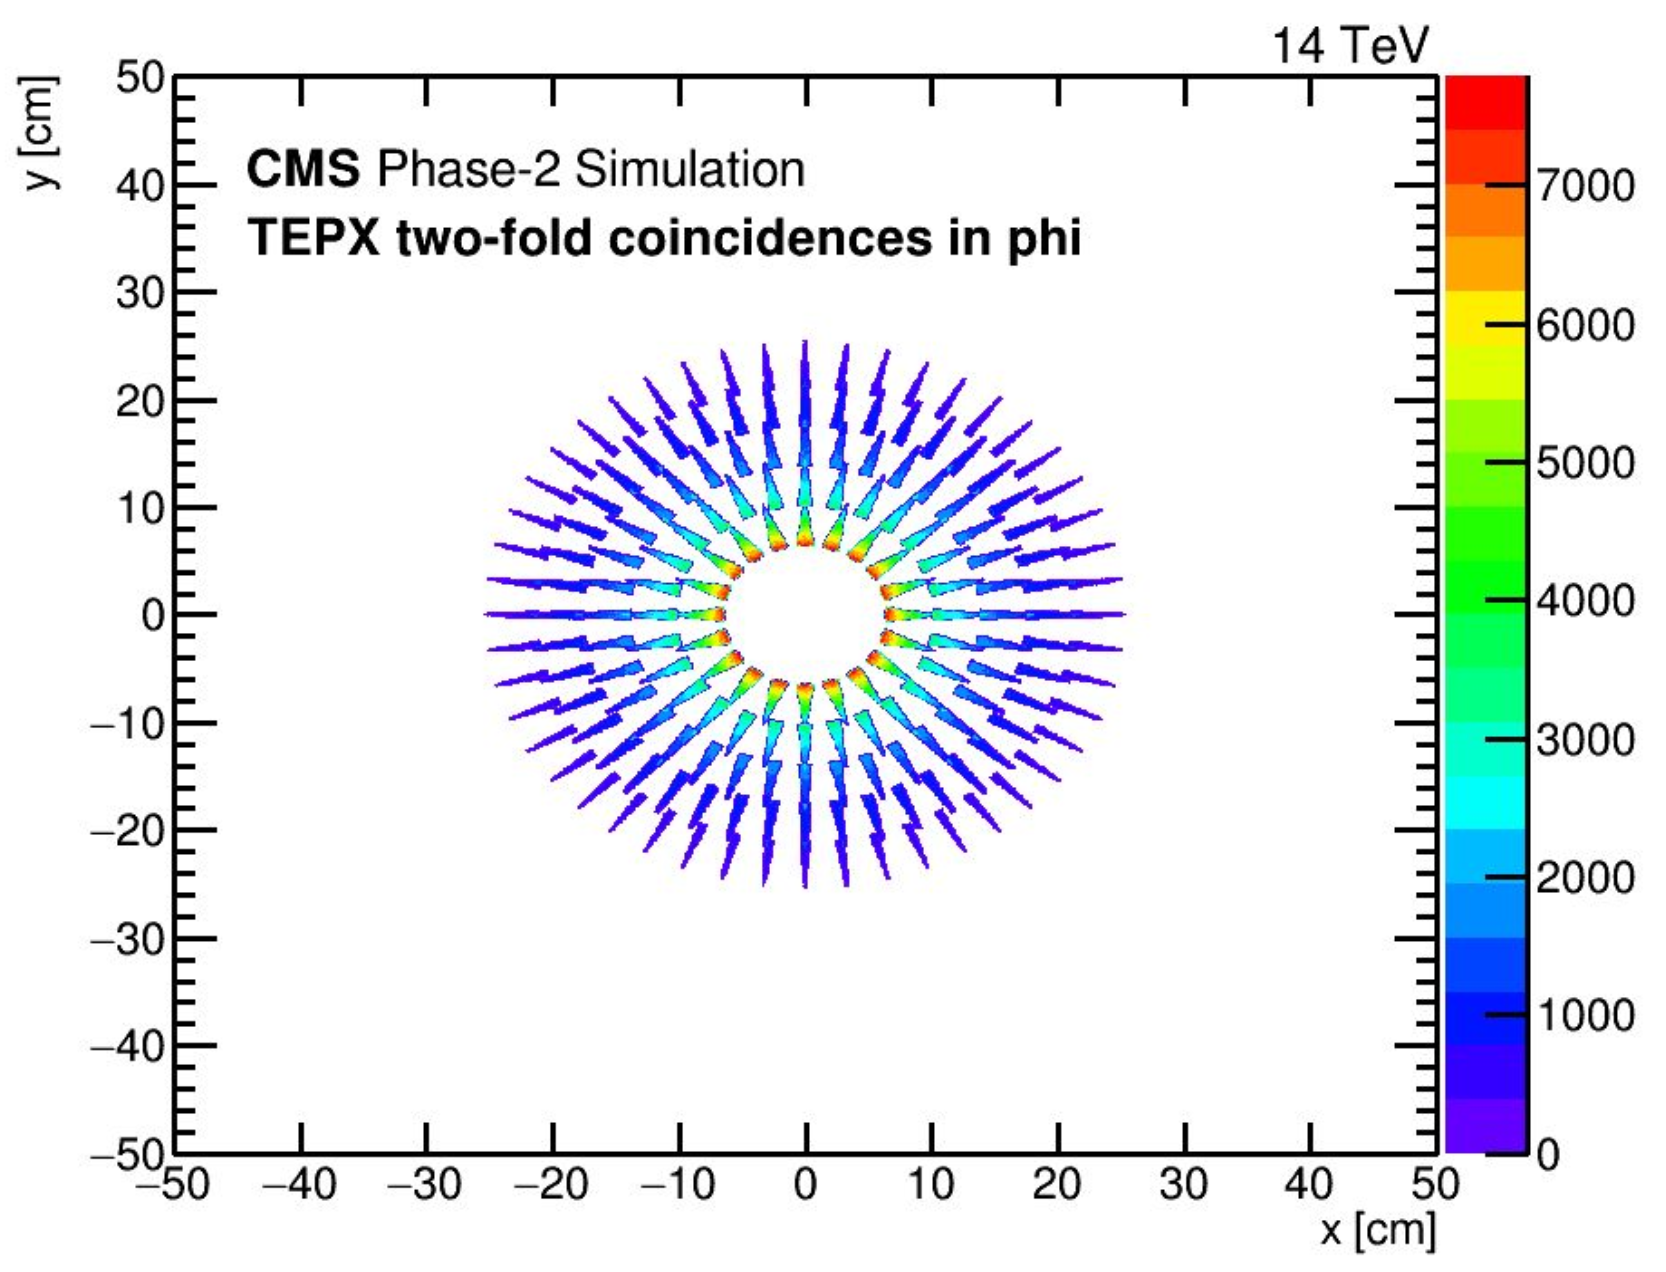
\includegraphics[width=1\textwidth]{ashish_thesis/twofoldinphi_sch.png}
\caption[Map Of Two Fold Coincidences in phi]{%                                                                                                                                                       
  Map of two fold coincidences in phi showing all module overlap regions.
}
\label{fig:cluster_ring_720}
\end{figure}


\newpage
Simlarly, we also studied two fold coincidences in r which arise from module overlaps between successive rings by only considering one to one module overlap between first two and last two layers in one TEPX double disk.  %Table \ref{table:two_fold_coincidences} categorizes various types of two-fold coincidences in r, observed in the TEPX detector. These coincidences are labeled from A to L and arise due to the module overlap in different layers within a single TEPX double disk. The 'dz' column quantifies the spatial separation along beam axis between the coinciding layers,  the z coordinates for Layers L1 to L4 within the TEPX detector is also mentioned. These coordinates provide a precise location for each layer, contributing to the understanding of where these two fold coincidences are likely to occur. The two fold coincidence in r map showing module overlap regions for different types is shown in Fig. \ref{fig:cluster_ring_770}.
 A one-to-one overlapping of modules is considered between L1L2 and L3L4 module overlap. %as shown in Fig. \ref{tab:my_label2}. 
 %The distributions for dr, dphi distribution depicting fake, true, total two fold coincidence in r for pileup 0.5 and 200 are shown in Fig. \ref{fig:cluster_ring_81} and \ref{fig:cluster_ring_82} respectively.
 Fit is done to pileup 0.5 distribution of true coincidences for both L1L2 and L3L4 coincidences in r .%as shown in Fig. \ref{fig:cluster_ring_83} and \ref{fig:cluster_ring_84}. 
 Fit results for all disks and rings are shown from  Table \ref{tab:my_label_55} to \ref{tab:my_label_50}. After applying all selections obtained from the fits, we plotted the XY map of two fold coincidences in r for L1L2 and L3L4 combined as shown in \ref{fig:cluster_ring_79}.


\begin{comment}

\begin{table}[H]
  \centering
  \caption[Two fold coincidences in r types]{Left: All type of two fold coincidences in r. Right: z coordinates for Layers L1 to L4.}
\begin{minipage}{0.45\textwidth}
    \centering
    \begin{tabular}{ccc}
    Modules & Type of Two Fold Coincidences & dz \\
    \hline
    A & R1L1-R2L2 & 0.4 \\
    B & R1L1-R2L4 & 1.2 \\
    C & R1L3-R2L4 & 0.4 \\
    D & R2L2-R3L3 & 0.4 \\
    E & R3L1-R2L2 & 0.4 \\
    F & R3L3-R2L4 & 0.4 \\
    G & R3L1-R4L2 & 0.4 \\
    H & R3L1-R4L4 & 1.2 \\
    I & R3L3-R4L4 & 0.4 \\
    J & R5L1-R4L2 & 0.4 \\
    K & R4L2-R5L3 & 0.4 \\
    L & R5L3-R4L4 & 0.4 \\
    \end{tabular}
\end{minipage}%
\hfill
\begin{minipage}{0.45\textwidth}
    \centering
    \begin{tabular}{cc}
    Layer & z-coordinate \\
    \hline
    Layer 1 (L1) & 264.4 \\
    Layer 2 (L2) & 264.8 \\
    Layer 3 (L3) & 265.2 \\
    Layer 4 (L4) & 265.6 \\
    \end{tabular}
\end{minipage}
\label{table:two_fold_coincidences}
\end{table}


\begin{figure}[!htp]
\centering
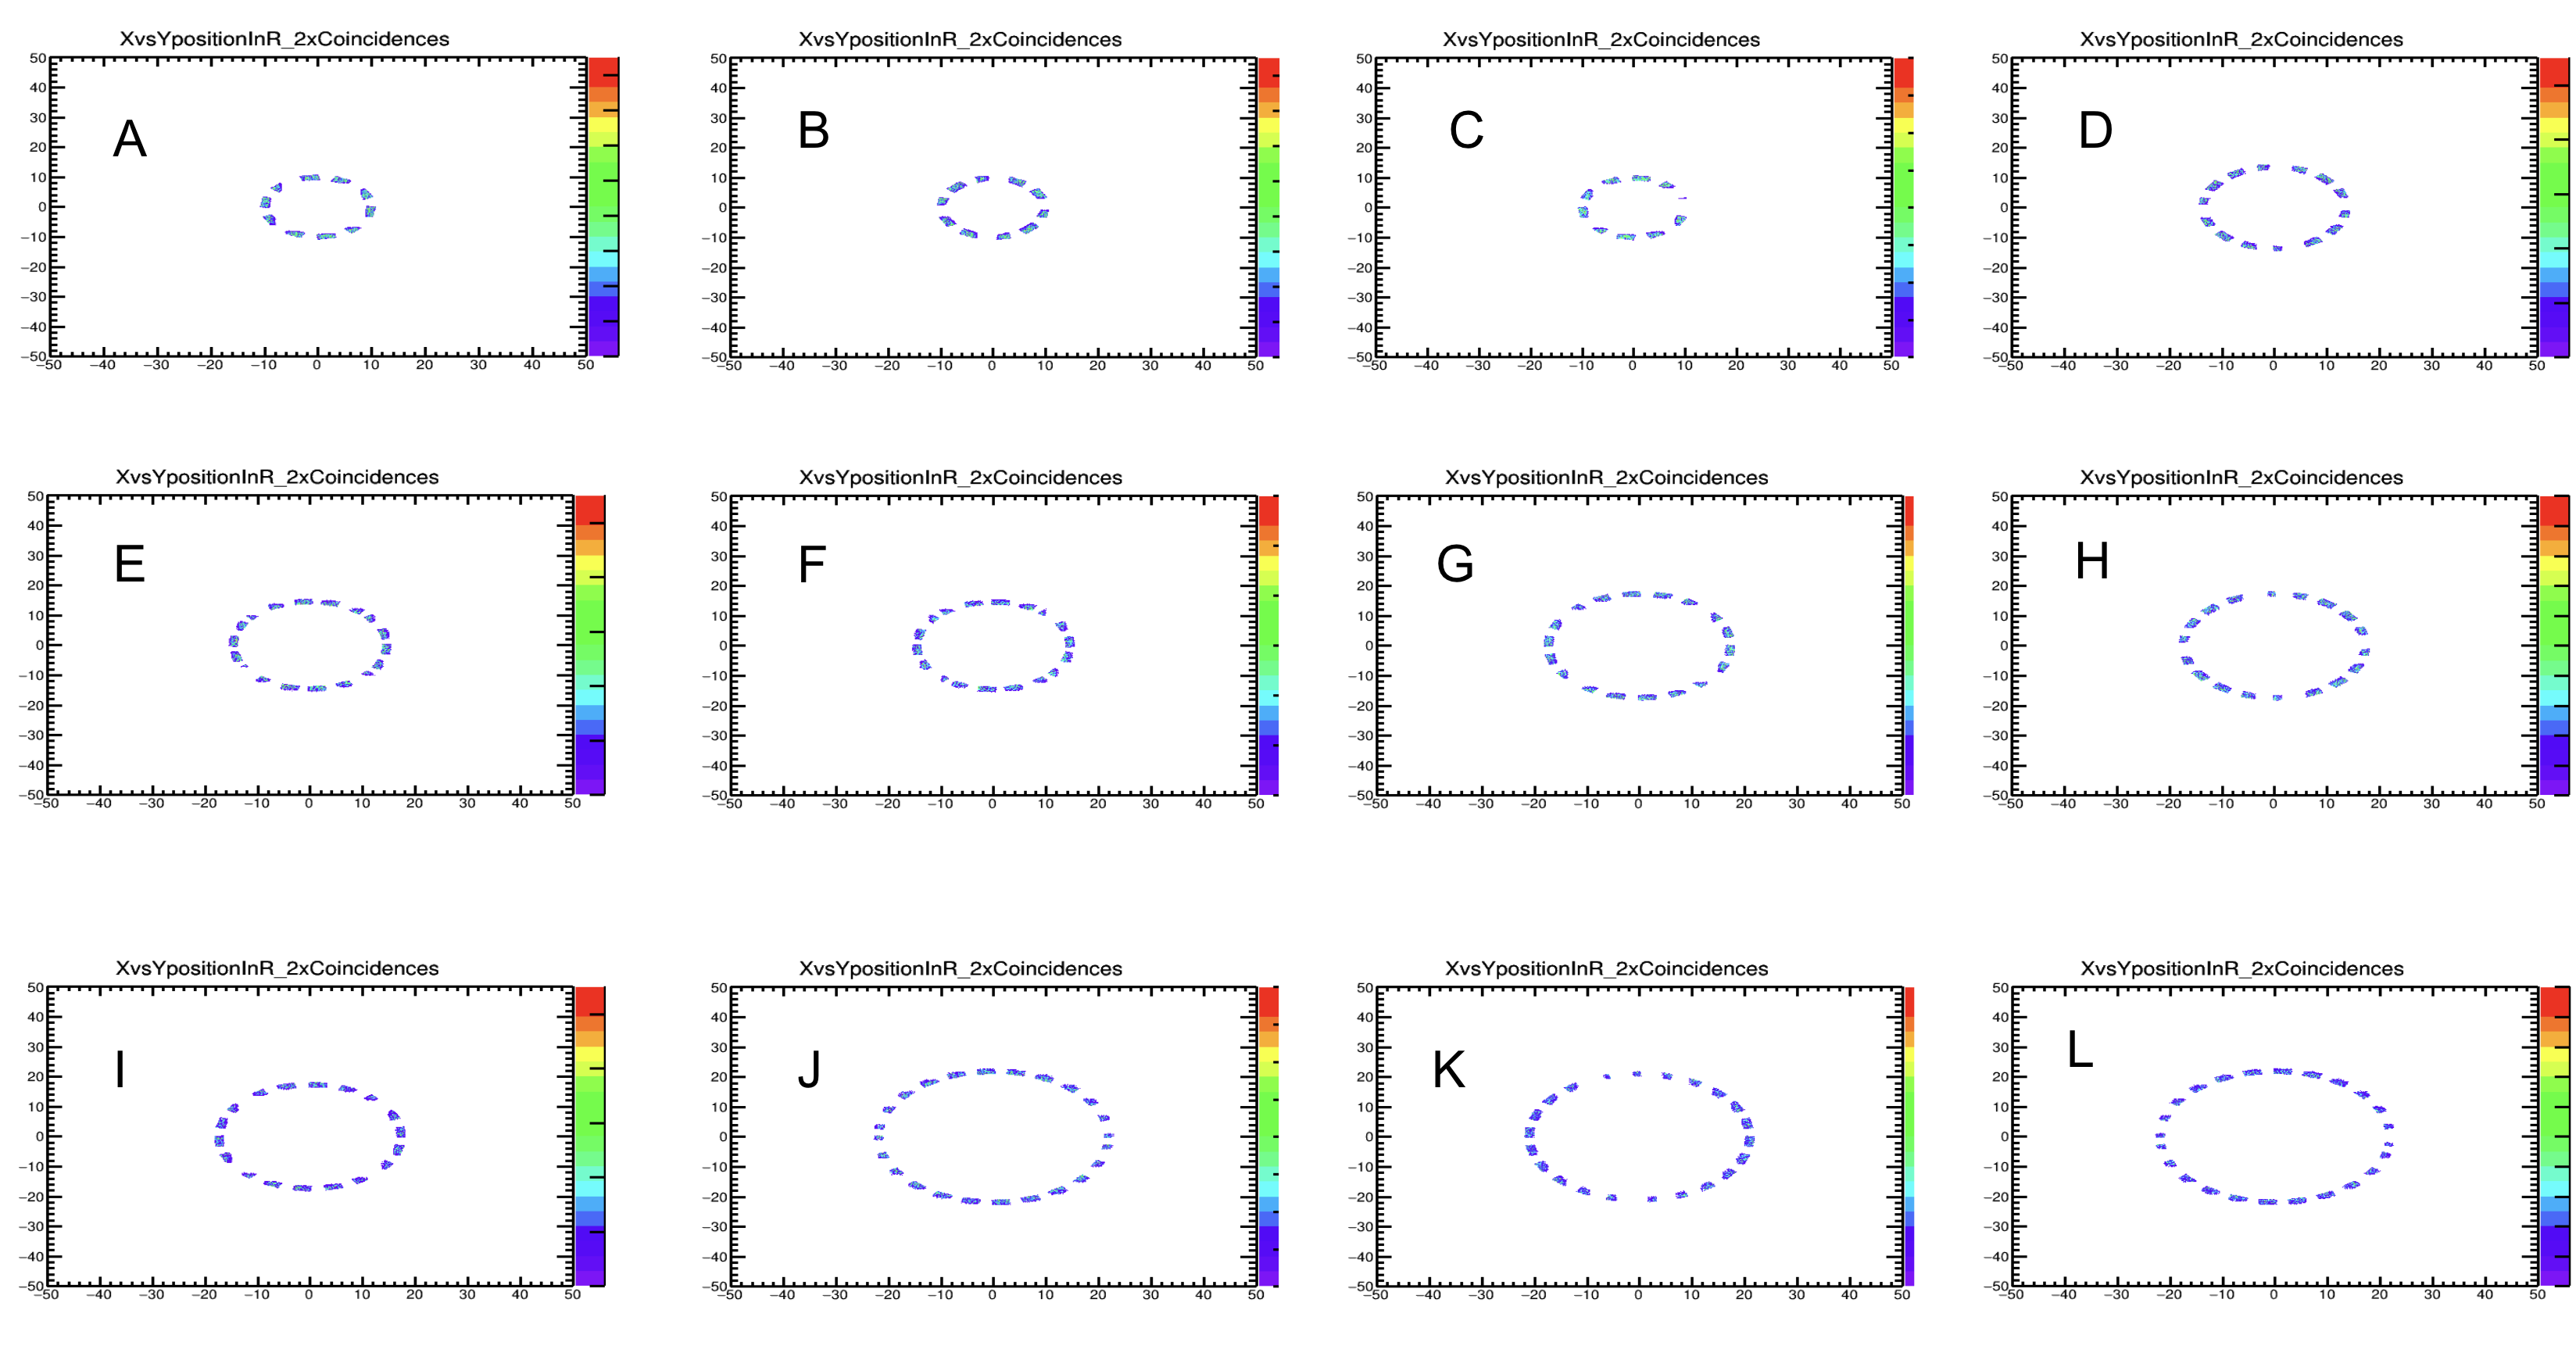
\includegraphics[width=1\textwidth]{ashish_thesis/twofoldinr_alltypes_diag.png}
\caption[Two Fold Coincidences in r types]{%                                                                                                                                                                                      
  Types of module overlap between different ring modules that can give rise to two fold coincidences in r.
}
\label{fig:cluster_ring_770}
\end{figure}

\begin{table}[H]
  \caption[Module mapping for two fold coincidenes in r]{Left: One to one module mapping in L1L2. Right: One to one module mapping in L3L4.}
  \begin{minipage}{0.45\linewidth}
    \centering
    %\caption{Left: One to one module mapping in L1L2. Right: One to one module mapping in L3L4}
    \begin{tabular}{cc}
      \textbf{R1L1} & \textbf{R2L2} \\
      \hline
      2 & 2 \\
      4 & 6 \\
      6 & 8 \\
      8 & 12 \\
      10 & 14 \\
      12 & 16 \\
      14 & 20 \\
      16 & 22 \\
      18 & 24 \\
      20 & 28 \\
    \end{tabular}
    %\label{tab:my_label1}
  \end{minipage}
  \hfill
  \begin{minipage}{0.45\linewidth}
    \centering
    %\caption{One to one module mapping in L3L4}
    \begin{tabular}{cc}
      \textbf{R1L3} & \textbf{R2L4} \\
      \hline
      1 & 1 \\
      3 & 5 \\
      5 & 7 \\
      7 & 9 \\
      9 & 13 \\
      11 & 15 \\
      13 & 19 \\
      15 & 21 \\
      17 & 23 \\
      19 & 27 \\
    \end{tabular}
    %\label{tab:my_label2}
  \end{minipage}
  \label{tab:my_label2}
\end{table}

\end{comment}

\begin{comment}

\begin{figure}[!htp]
\centering
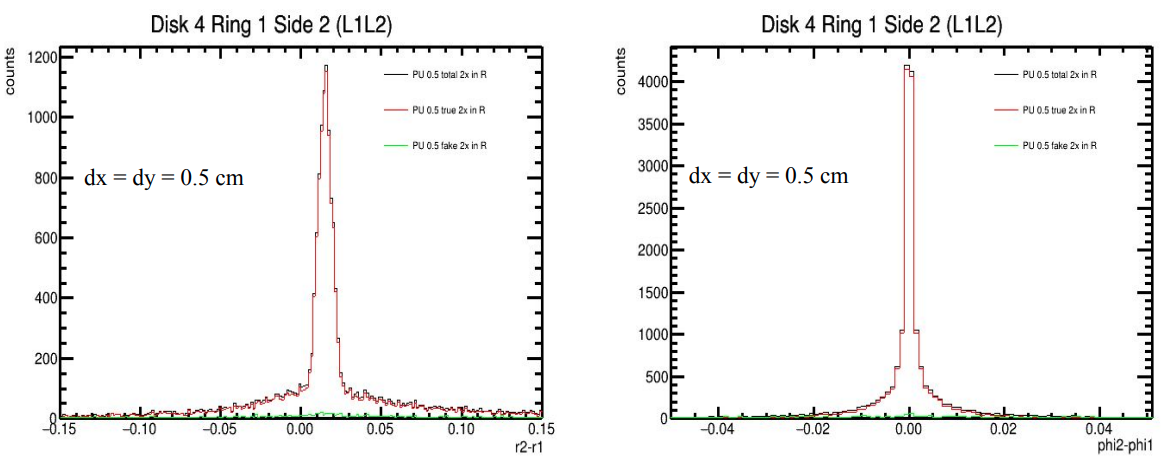
\includegraphics[width=1\textwidth]{ashish_thesis/l1l2_dr_dphi_D4R1S2.png}
\caption[D4R1 Two-Fold Coincidences vs. dr & dphi (PU 0.5)]{%
   PU 0.5 D4R1 total, true, fake two fold coincidences  in r as a function of dr, dphi variables.
}
\label{fig:cluster_ring_81}
\end{figure}

\begin{figure}[!htp]
\centering
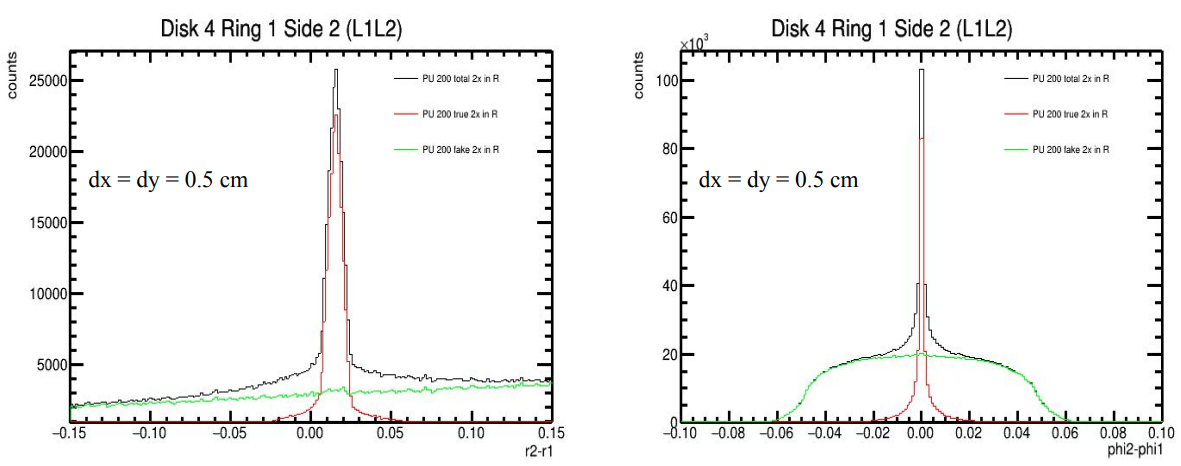
\includegraphics[width=1\textwidth]{ashish_thesis/l1l2_drdphi_2xinr_PU200.png}
\caption[D4R1 Two-Fold Coincidences vs. dr & dphi (PU 200)]{%
   PU 200 D4R1 total, true, fake two fold coincidences  in r as a function of dr, dphi variables.
}
\label{fig:cluster_ring_82}
\end{figure}

\endn{comment}

\begin{comment}

\begin{figure}[!htp]
\centering
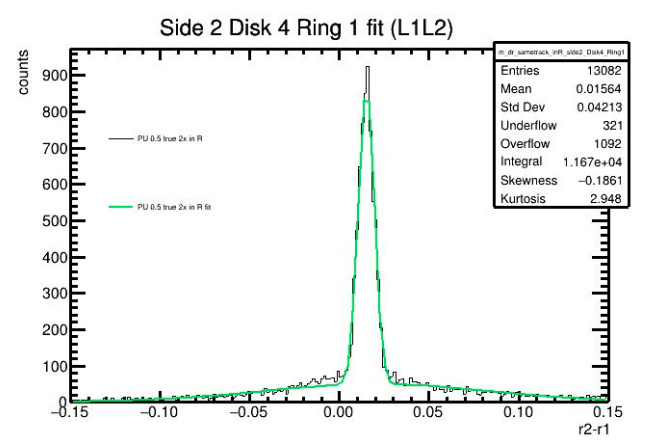
\includegraphics[width=1\textwidth]{ashish_thesis/fit_l1l2_dr_2xinr.png}
\caption[Fit L1L2 Two Fold Coincidences in r]{%
   Fit L1L2 two fold coincidences in R.
}
\label{fig:cluster_ring_83}
\end{figure}


\begin{table}[H]
  \centering
  \caption{Fit parameters for dr}
\begin{tabular}{ccc}
\textbf{Parameter Name} & \textbf{Value} & \textbf{Error} \\ 
\hline
p0 & 8.25e+02 & 1.40e+01 \\ 
p1 & 1.49e-02 & 6.52e-05 \\ 
p2 & 4.44e-03 & 5.61e-05 \\ 
p3 & 4.94e+01 & 1.18e+00 \\ 
p4 & 2.04e-02 & 9.87e-04 \\ 
p5 & 6.35e-02 & 1.14e-03 \\ 
\end{tabular}
\label{tab:my_label3}
\end{table}


\begin{figure}[!htp]
\centering
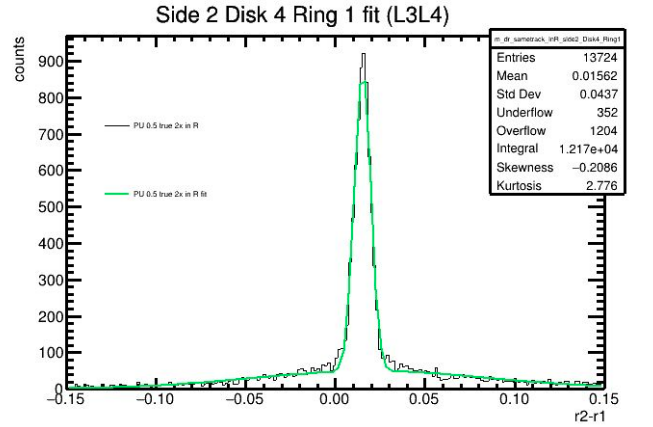
\includegraphics[width=1\textwidth]{ashish_thesis/fit_l3l4_dr_2xinr.png}
\caption[Fit L3L4 Two Fold Coincidences in r]{%
   Fit L3L4 two fold coincidences in r.
}
\label{fig:cluster_ring_84}
\end{figure}


\begin{table}[H]
  \centering
  \caption{Fit parameters for dr}
\begin{tabular}{ccc}
\textbf{Parameter Name} & \textbf{Value} & \textbf{Error} \\ 
\hline
p0 & 8.33e+02 & 1.43e+01 \\ 
p1 & 1.50e-02 & 6.56e-05  \\ 
p2 & 4.57e-03  & 6.01e-05 \\
p3 & 4.95e+01 & 1.17e+00 \\
p4 & 2.02e-02 & 1.04e-03  \\  
p5 & 6.68e-02 & 1.24e-03  \\ 
\end{tabular}
\label{tab:my_label6}
\end{table}

\end{comment}

%\begin{table}[h]
 % \centering
  %\caption{Fit parameters for dphi}
%\begin{tabular}{ccc}
%\textbf{Parameter Name} & \textbf{Value} & \textbf{Error} \\ 
%\hline
%p0 & 1.263e+03 & 2.52e+01 \\ 
%p1 & 0.00e+00 & fixed \\ 
%p2 & 4.510e-04 & 7.25e-06 \\
%\end{tabular}
%\label{tab:my_label10}
%\end{table}


\begin{table}[H]
  \centering
  \caption[dr mean values (L1L2)]{dr mean values obtained from fit for all disks and rings for coincidences in r in layers L1L2}
\begin{tabular}{ccccc}
 & \multicolumn{4}{c}{\textbf{Ring}} \\
\textbf{Disk} & \textbf{1} & \textbf{2} & \textbf{3} & \textbf{4} \\
\hline
%-4 & 0.0230881 & 0.0309854 & 0.0387241 & 0.0464962 \\ 
%-3 & 0.0199761 & 0.0270206 & 0.0338467 & 0.0403068 \\ 
%-2 & 0.017385  & 0.0233397 & 0.0294101 & 0.0348779 \\ 
%-1 & 0.0150614 & 0.0202725 & 0.0255259 & 0.0303849 \\
1 & 0.0229736 & 0.0311421 & 0.0390871 & 0.0468038 \\
2 & 0.0202136 & 0.0268963 & 0.0337796 & 0.040398 \\
3 & 0.0174894 & 0.0233893 & 0.0293971 & 0.0351501 \\
4 & 0.0149661 & 0.020194  & 0.0255051 & 0.0305483 \\
\end{tabular}
\label{tab:my_label_55}
\end{table}


\begin{table}[H]
  \centering
  \caption[dphi cut values (L1L2)]{dphi standard deviation values obtained from fit for all disks and rings for coincidences in r in layers L1L2}
\begin{tabular}{ccccc}
 & \multicolumn{4}{c}{\textbf{Ring}} \\
\textbf{Disk} & \textbf{1} & \textbf{2} & \textbf{3} & \textbf{4} \\
\hline
%-4 & 0.000628313 & 0.000828659 & 0.000975585 & 0.00101984 \\ 
%-3 & 0.000545699 & 0.000722289 & 0.00081899 & 0.000918094 \\ 
%-2 & 0.000495422 & 0.000649127 & 0.000754224 & 0.000839347 \\ 
%-1 & 0.000451069 & 0.000604104 & 0.000689508 & 0.000755603 \\
1 & 0.000627781 & 0.000814669 & 0.000941641 & 0.0010221 \\
2 & 0.000573352 & 0.000761853 & 0.000851161 & 0.000901014 \\
3 & 0.000523361 & 0.000662691 & 0.000778358 & 0.000834924 \\
4 & 0.000471669 & 0.000589938 & 0.000692007 & 0.000750302 \\
\end{tabular}
\label{tab:my_label_54}
\end{table}


\begin{table}[H]
  \centering
  \caption[dr cut values (L1L2)]{dr standard deviation values obtained from fit for all disks and rings for coincidences in r in layers L1L2}
\begin{tabular}{ccccc}
 & \multicolumn{4}{c}{\textbf{Ring}} \\
\textbf{Disk} & \textbf{1} & \textbf{2} & \textbf{3} & \textbf{4} \\
\hline
%-4 & 0.00458531 & 0.00466448 & 0.00486059 & 0.0052905 \\ 
%-3 & 0.00444971 & 0.0046465 & 0.00472138 & 0.00490022 \\ 
%-2 & 0.00453556 & 0.00471864 & 0.00465781 & 0.00503102 \\ 
%-1 & 0.00457346 & 0.00458345 & 0.00478342 & 0.00497171 \\
1 & 0.00448255 & 0.00445856 & 0.00474102 & 0.0051553 \\
2 & 0.00442349 & 0.00472485 & 0.00474663 & 0.0050426 \\
3 & 0.00450002 & 0.0045179 & 0.00492058 & 0.00494887 \\
4 & 0.00444657 & 0.00468584 & 0.00493828 & 0.00488064 \\
\end{tabular}
\label{tab:my_label_53}
\end{table}


\begin{table}[H]
  \centering
  \caption[dphi cut values (L3L4)]{dphi standard deviation values obtained from fit for all disks and rings for coincidences in r in layers L3L4}
\begin{tabular}{ccccc}
 & \multicolumn{4}{c}{\textbf{Ring}} \\
\textbf{Disk} & \textbf{1} & \textbf{2} & \textbf{3} & \textbf{4} \\
\hline
%-4 & 0.00448255 & 0.00445856 & 0.00474102 & 0.0051553 \\ 
%-3 & 0.00442349 & 0.00472485 & 0.00474663 & 0.0050426 \\ 
%-2 & 0.00450002 & 0.0045179 & 0.00492058 & 0.00494887 \\ 
%-1 & 0.00444657 & 0.00468584 & 0.00493828 & 0.00488064 \\
1 & 0.00458531 & 0.00466448 & 0.00486059 & 0.0052905 \\
2 & 0.00444971 & 0.0046465 & 0.00472138 & 0.00490022 \\
3 & 0.00453556 & 0.00471864 & 0.00465781 & 0.00503102 \\
4 & 0.00457346 & 0.00458345 & 0.00478342 & 0.00497171 \\
\end{tabular}
\label{tab:my_label_52}
\end{table}



\begin{table}[H]
  \centering
  \caption[dphi cut values (L3L4)]{dphi standard deviation values obtained from fit for all disks and rings for coincidences in r in layers L3L4}
\begin{tabular}{ccccc}
 & \multicolumn{4}{c}{\textbf{Ring}} \\
\textbf{Disk} & \textbf{1} & \textbf{2} & \textbf{3} & \textbf{4} \\
\hline
%-4 & 0.000627781 & 0.000814669 & 0.000941641 & 0.0010221 \\ 
%-3 & 0.000573352 & 0.000761853 & 0.000851161 & 0.000901014 \\ 
%-2 & 0.000523361 & 0.000662691 & 0.000778358 & 0.000834924 \\ 
%-1 & 0.000471669 & 0.000589938 & 0.000692007 & 0.000750302 \\
1 & 0.000628313 & 0.000828659 & 0.000975585 & 0.00101984 \\
2 & 0.000545699 & 0.000722289 & 0.00081899 & 0.000918094 \\
3 & 0.000495422 & 0.000649127 & 0.000754224 & 0.000839347 \\
4 & 0.000451069 & 0.000604104 & 0.000689508 & 0.000755603 \\
\end{tabular}
\label{tab:my_label_51}
\end{table}


\begin{table}[H]
  \centering
  \caption[dr mean values (L3L4)]{dr mean values obtained from fit for all disks and rings for coincidences in r in layers L3L4}
\begin{tabular}{ccccc}
 & \multicolumn{4}{c}{\textbf{Ring}} \\
\textbf{Disk} & \textbf{1} & \textbf{2} & \textbf{3} & \textbf{4} \\
\hline
%-4 & 0.0229736 & 0.0311421 & 0.0390871 & 0.0468038 \\ 
%-3 & 0.0202136 & 0.0268963 & 0.0337796 & 0.040398 \\ 
%-2 & 0.0174894 & 0.0233893 & 0.0293971 & 0.0351501 \\ 
%-1 & 0.0149661 & 0.020194 & 0.0255051 & 0.0305483 \\
1 & 0.0230881 & 0.0309854 & 0.0387241 & 0.0464962 \\
2 & 0.0199761 & 0.0270206 & 0.0338467 & 0.0403068 \\
3 & 0.017385 & 0.0233397 & 0.0294101 & 0.0348779 \\
4 & 0.0150614 & 0.0202725 & 0.0255259 & 0.0303849 \\
\end{tabular}
\label{tab:my_label_50}
\end{table}

\begin{comment}

\begin{figure}[!htp]
\centering
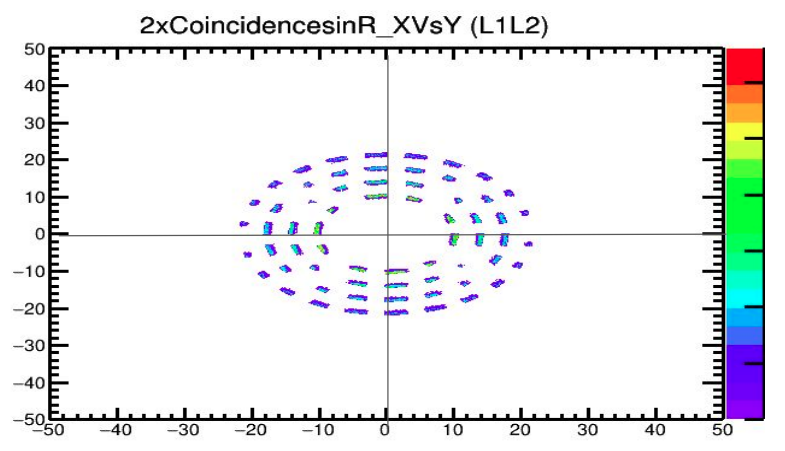
\includegraphics[width=1\textwidth]{ashish_thesis/l1l2_2xinr.png}
\caption[L1L2 Module Overlap Map for Two Fold Coincidences in r]{%                                                                                                                                   
   Module overlap map in L1L2 layers for two fold coincidences in r.
}
\label{fig:cluster_ring_77}
\end{figure}

\begin{figure}[!htp]
\centering
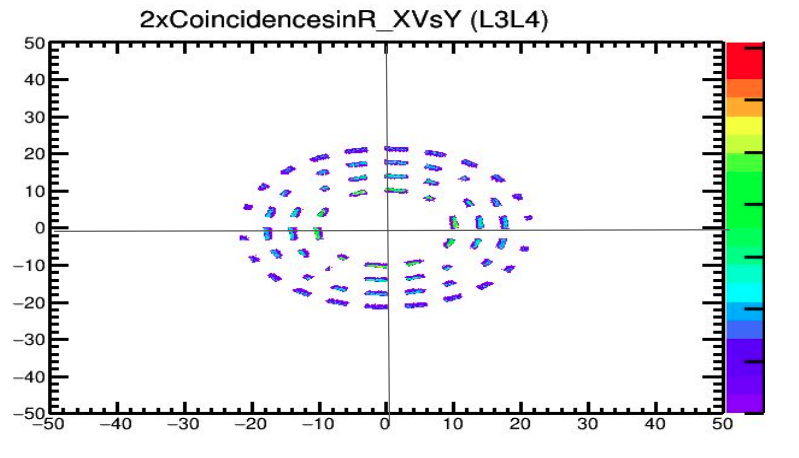
\includegraphics[width=1\textwidth]{ashish_thesis/l3l4_2xinr.png}
\caption[L3L4 Module Overlap Map for Two Fold Coincidences in r]{%                                                                                                                                                        
   Module overlap map in L3L4 layers for two fold coincidences in r.
}
\label{fig:cluster_ring_78}
\end{figure}

\end{comment}

\begin{figure}[!htp]
\centering
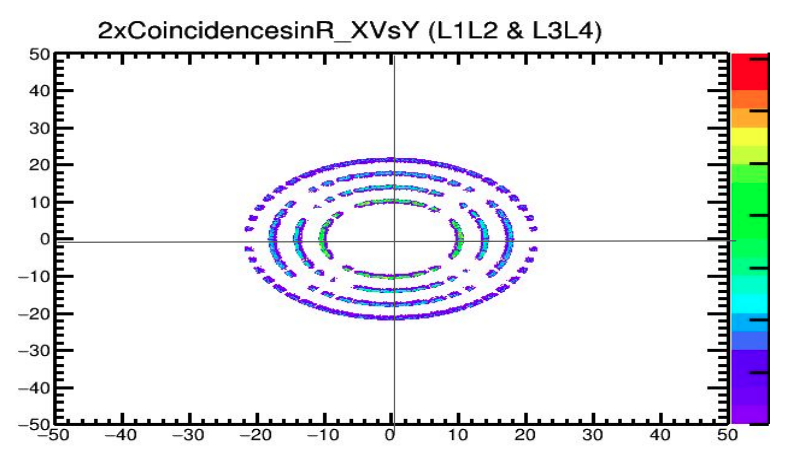
\includegraphics[width=1\textwidth]{ashish_thesis/l1l2_l3l4_2xinr.png}
\caption[L1L2 and L3L4 Module Overlap Map for Two Fold Coincidences in r]{%                                                                                                                                                                                      
   Module overlap map in L1L2 and L3L4 layers for two fold coincidences in r.
}
\label{fig:cluster_ring_79}
\end{figure}


\newpage
The new algorithm is able to remove physics noise at high pileup as can be seen from the high efficiency values and low fake rates for Disk 4 all rings and all pileup samples as shown in Table \ref{tab:sample}, \ref{tab:sample_1} and \ref{tab:sample_2}.

\begin{table}[H]
  \centering
  \caption{Fake rate for Disk 4 all rings}
  \begin{tabular}{cc}
    \textbf{Disk 4} & \textbf{Fake two fold coincidence rate (\%)} \\
    \hline
    Ring 1 &  1.1\\
    Ring 2 &  1.9\\
    Ring 3 &  2.0\\
    Ring 4 &  2.5\\
    Ring 5 &  2.3\\
  \end{tabular}
  \label{tab:sample}
\end{table}


\begin{table}[H]
  \centering
  \caption{TEPX two fold coincidences fake rate}
\begin{tabular}{cccc}
\textbf{Pileup} & \textbf{Fake two fold} & \textbf{Fake two fold} & \textbf{Fake two} \\
\textbf{} & \textbf{coincidence in phi} & \textbf{coincidence in R} & \textbf{fold coincidence} \\
\hline
0.5  &  0.78& 0.99 & 0.83 \\
1& 0.79 &  1.01 &0.85\\
1.5 &  0.80& 1.02 & 0.86 \\
2 & 0.79 & 1.02&  0.84\\
10 &  0.83&  1.04&  0.88\\
30&  0.94&  1.09&  0.98\\
50 &  1.04&  1.14&  1.07\\
100  & 1.31 & 1.29& 1.31\\
140  & 1.53 & 1.41& 1.50\\
200   & 1.85 & 1.57 &1.78\\
\end{tabular}
\label{tab:sample_1}
\end{table}


\begin{table}[H]
  \centering
  \caption{TEPX two coincidences efficiency}
\begin{tabular}{cccc}
\textbf{Pileup} & \textbf{Efficiency for two} & \textbf{Efficiency for Fake} & \textbf{Efficiency for two} \\
& \textbf{fold coincidence in phi} & \textbf{two fold coincidence in R} & \textbf{fold coincidence} \\
\hline
0.5  & 99.21 &99.00  &99.16  \\
1& 99.20 &98.98  & 99.14 \\
1.5 & 99.19 & 98.97 & 99.13 \\
2& 99.20 & 98.97 & 99.13 \\
10 & 99.16 & 98.95 & 99.11 \\
30& 99.05 & 98.90 & 99.01 \\
50 & 98.95 & 98.85 & 98.92 \\
100& 98.68 & 98.70 & 98.68 \\
140& 98.46 & 98.58 & 98.49 \\
200 &98.14  & 98.42 &98.21  \\
\end{tabular}
\label{tab:sample_2}
\end{table}

%Ratio of the integrals for fake & total coincidence for dr & dphi distributions is 3454/145988 = 0.023


It is important to study how the number of two fold coincidences after final selections change with pileup for precise luminosity measurement. Number of two fold coincidences increases with pileup. Distribution of two fold coincidences for TEPX Disk 4 Ring 1 for all pileup values is shown in Fig. \ref{fig:tepx_coin_allPU}. For pileup 200, mean two fold coincidences is around 270. Under vdM conditions, it range from 0 to 13. The new algorithm is able to suppress non-linearity at high pileup values as shown from Fig.  1.17 to Fig. 1.24.

\begin{figure}[H]
  \centering
  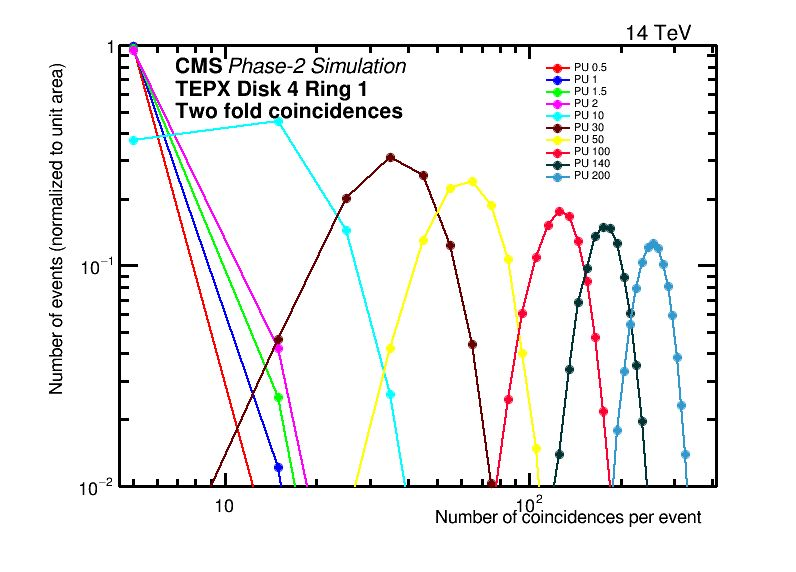
\includegraphics[width=0.7\columnwidth]{ashish_thesis/tepx_D4R1_coin_allpu_1.png}
  \caption[TEPX D4R1 Two Fold Coincidences All Pileup]{Distribution of number of two fold coincidences for TEPX Disk 4 Ring 1 for all pileup values.}
  \label{fig:tepx_coin_allPU}
\end{figure}


\begin{figure}[H]
  \centering
  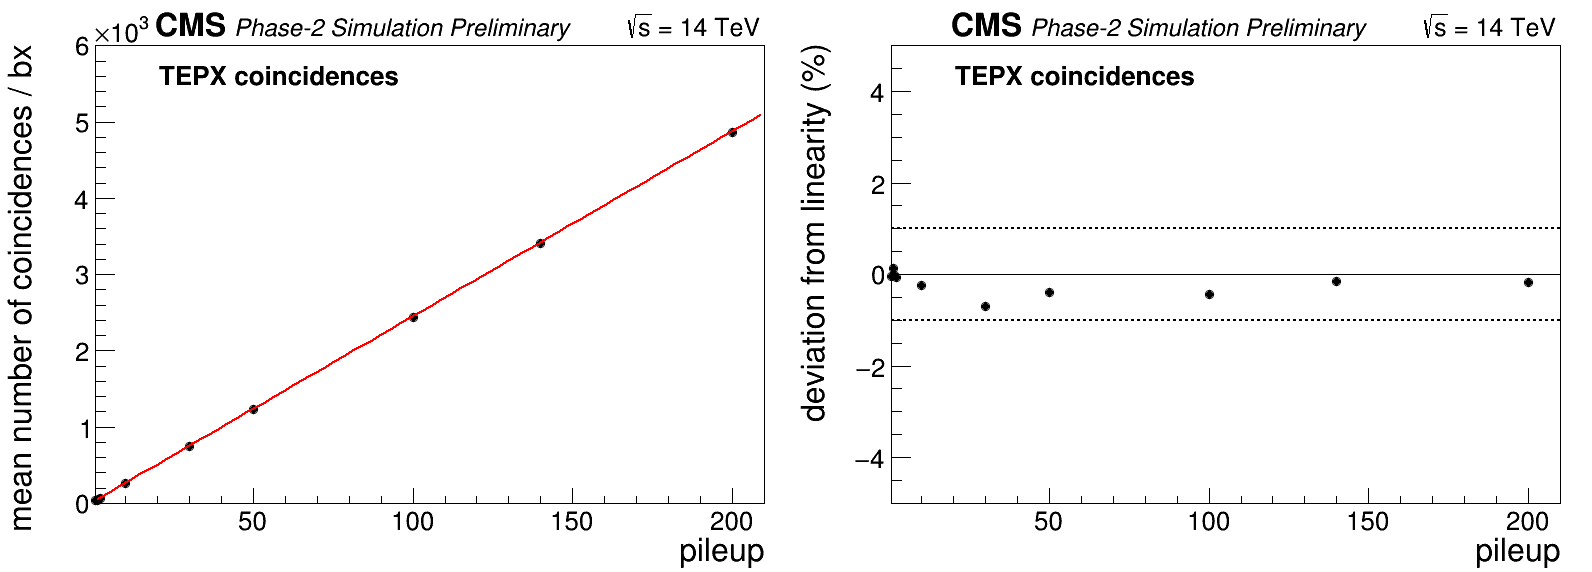
\includegraphics[width=1 \columnwidth]{ashish_thesis/totalcoincidences.png}
  \caption[TEPX Two Fold Coincidences Fit And Residual]{Left: Simulated mean number of coincidences in $\phi$ and r for all entire TEPX detector as a function of pileup. A line is fitted between pileup values of 0 and 2, and then extrapolated up to a pileup of 200. Right: Deviation from linearity for coincidence in $\phi$ and r for entire TEPX detector. The non-linearity is calculated as the relative difference between the data points and the values of the fit function at the respective pileup value. Non-linearity is within 1 \% for entire pileup range. Pileup 200 corresponds to High Luminosity (HL)-LHC environment.}
  \label{fig:CMS}
\end{figure}


\begin{figure}[H]
  \centering
  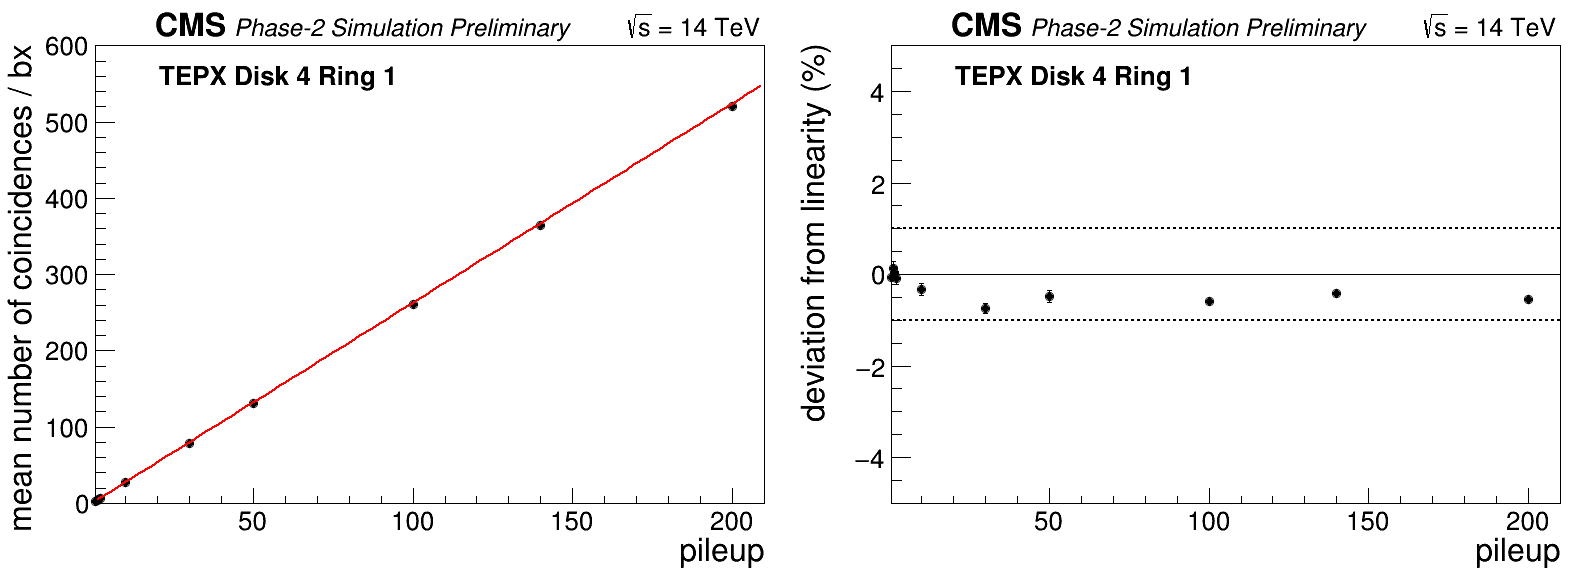
\includegraphics[width=1\columnwidth]{ashish_thesis/totalcoincidencesD4R1.png}
  \caption[Two Fold Coincidences for Disk 4 Ring 1 Fit And Residual]{Left: Simulated mean number of coincidences in $\phi$ and r for TEPX Disk 4 Ring 1 as a function of pileup. Right: Deviation from linearity for coincidences in $\phi$ and r for TEPX Disk 4 Ring 1. The non-linearity is calculated as the relative difference between the data points and the values of the fit function at the respective pileup value.}
  \label{fig:CMS}
\end{figure}


\begin{figure}[H]
  \centering
  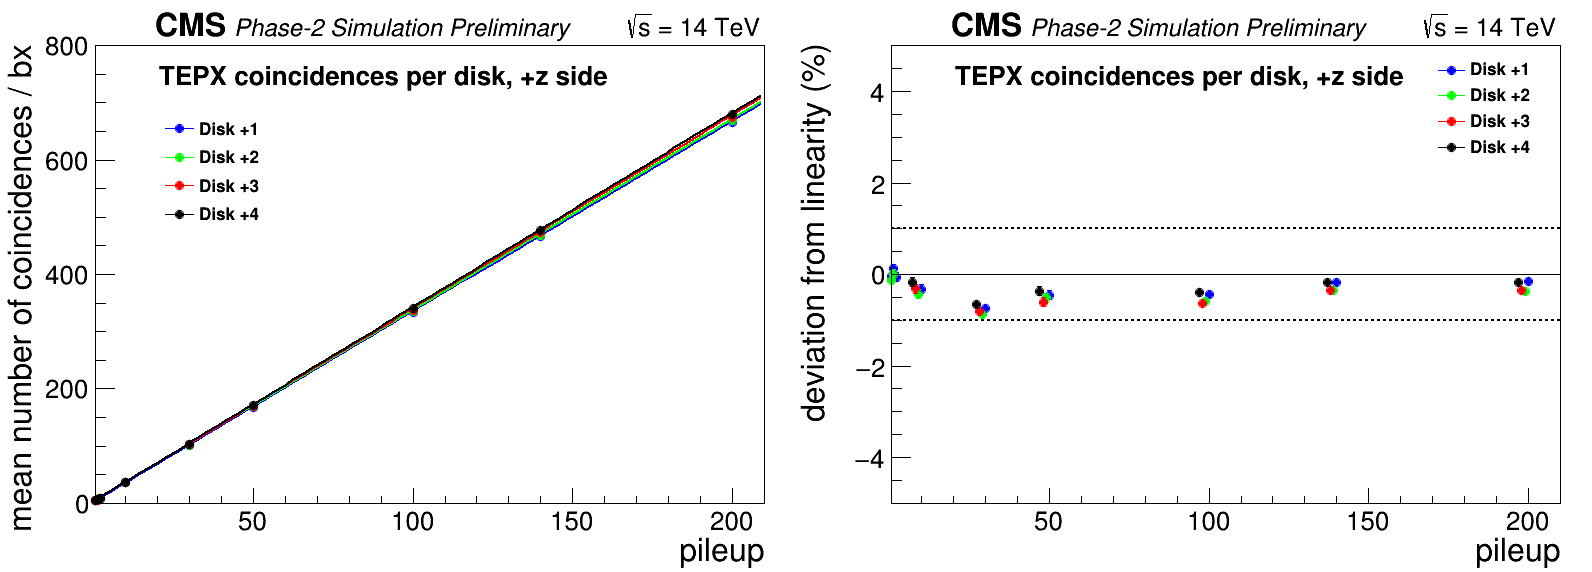
\includegraphics[width=1\columnwidth]{ashish_thesis/coincidencesperdisk+z.png}
  \caption[Two Fold Coincidences Per Disk Fit And Residual]{Left: Simulated mean number of coincidences in $\phi$ and r for +z side TEPX disks as a function of pileup. Right: Deviation from linearity for coincidences in $\phi$ and r for +z side TEPX disks.}
  \label{fig:CMS}
\end{figure}


\begin{figure}[H]
  \centering
  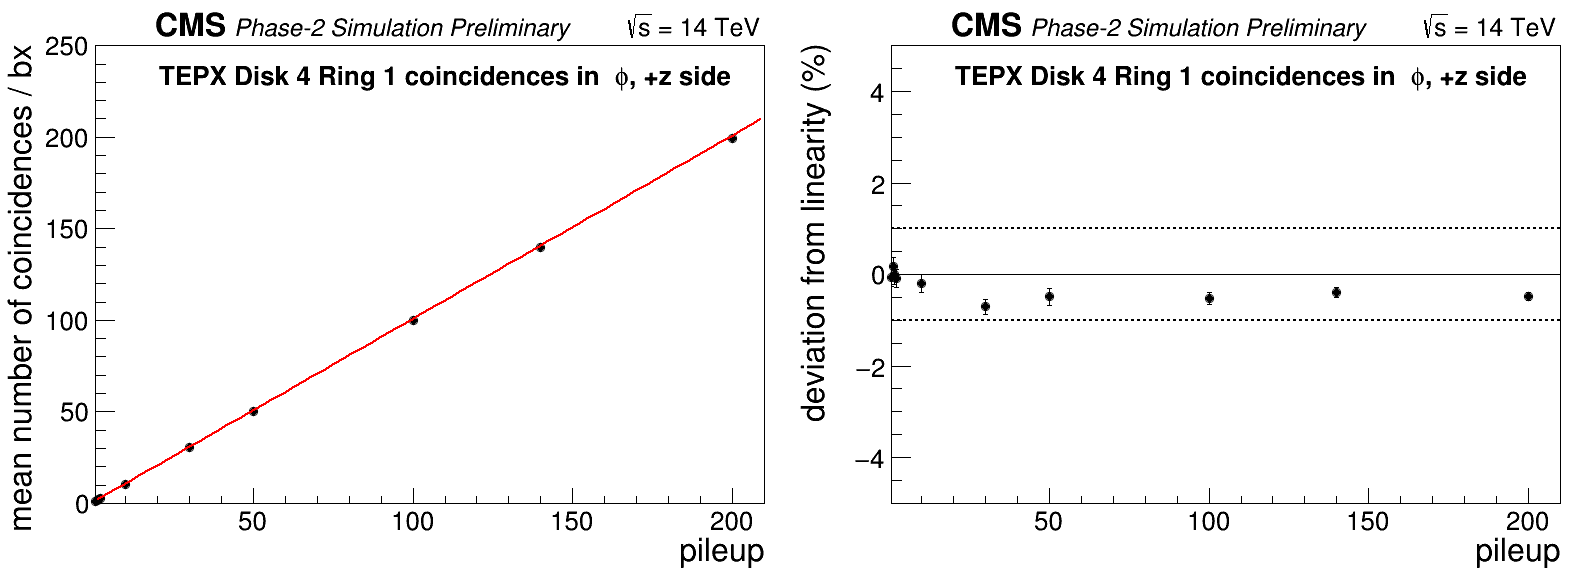
\includegraphics[width=1\columnwidth]{ashish_thesis/coincidencesinphiD4R1z+.png}
  \caption[Two Fold Coincidences in phi for Disk 4 Ring 1 Fit And Residual]{Left: Simulated mean number of coincidences in $\phi$ for TEPX +z side Disk 4 Ring 1 as a function of pileup. Right: Deviation from linearity for coincidences in $\phi$ for TEPX +z side Disk 4 Ring 1. The non-linearity is calculated as the relative difference between the data points and the values of the fit function at the respective pileup value.}
  \label{fig:CMS}
\end{figure}



\begin{figure}[H]
  \centering
  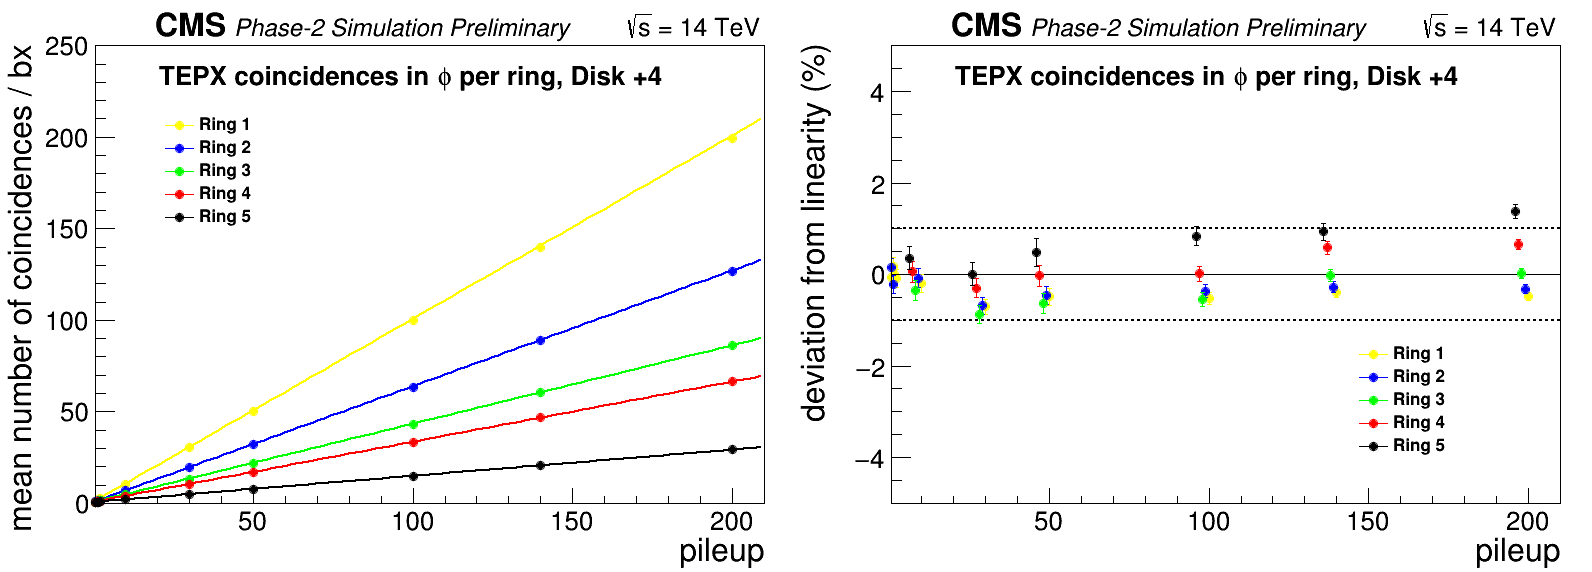
\includegraphics[width=1\columnwidth]{ashish_thesis/coincidencesinphiperringD+4.png}
  \caption[Two fold coincidences in phi per ring Fit And Residual]{Left: Simulated mean number of coincidences in $\phi$ for +z side TEPX Disk 4 per ring as a function of pileup. Ring 1 has highest slope and Ring 5 has least slope. Right: Deviation from linearity for coincidences in $\phi$ for +z side TEPX Disk 4 per ring. Non-linearity is within 1\% for all rings over entire pileup range.}
  \label{fig:CMS}
\end{figure}


\begin{figure}[H]
  \centering
  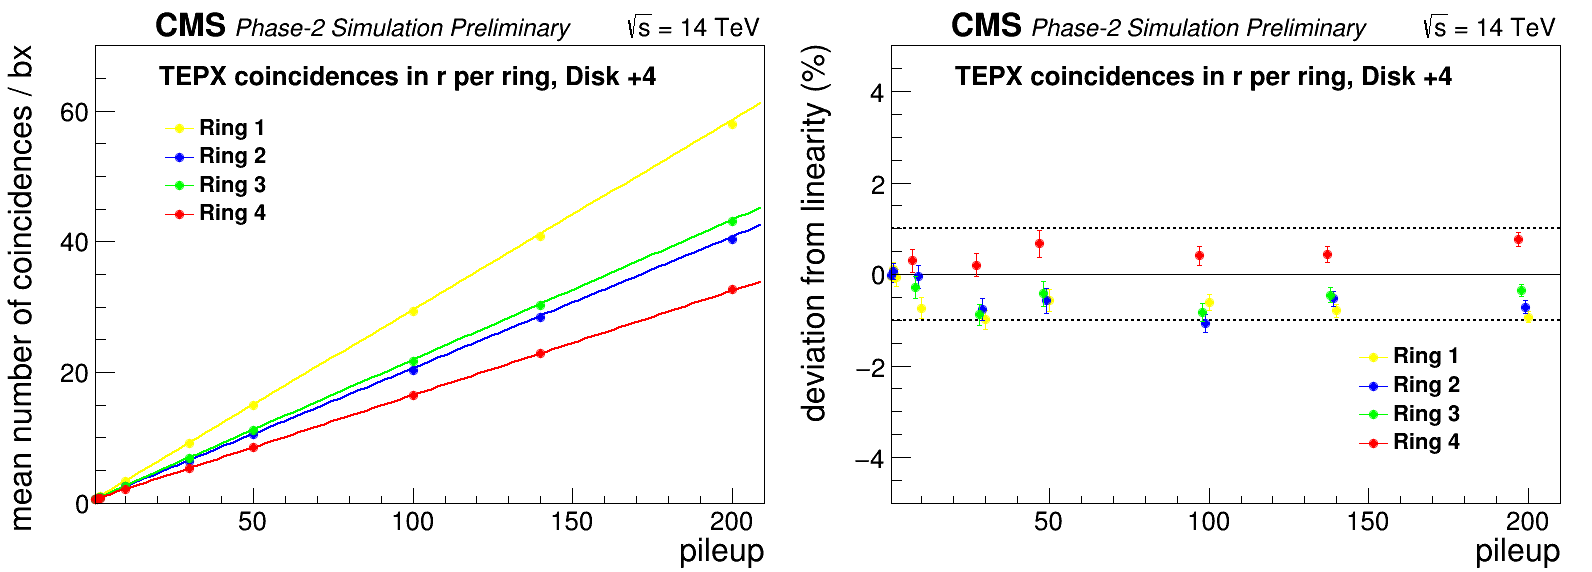
\includegraphics[width=1\columnwidth]{ashish_thesis/coincidencesinrperringD+4.png}
  \caption[Two Fold Coincidences in r Per Ring Fit And Residual]{Left: Simulated mean number of coincidences in r for +z side TEPX Disk 4 per ring as a function of pileup. Ring 1 has highest slope and Ring 5 has least slope. Right: Deviation from linearity for coincidences in r for +z side TEPX Disk 4 per ring. Non-linearity is within $1\%$ for all rings over entire pileup range.}
  \label{fig:CMS_999}
\end{figure}



\begin{comment}
  
For Disk 4 Ring 1, fake coincidences are randomly distributed and true coincidences are localized in the middle of the distribution as shown in Fig. \ref{fig:cluster_ring_20}.  For Disk 4 Ring 5, fake coincidence are randomly distributed. True coincidences are localized in the middle of the distribution. Compared to Ring 1, there are less true coincidences in the middle part of the distribution as shown in Fig. \ref{fig:cluster_ring_21}.


\begin{figure}[!htp]
  \centering
  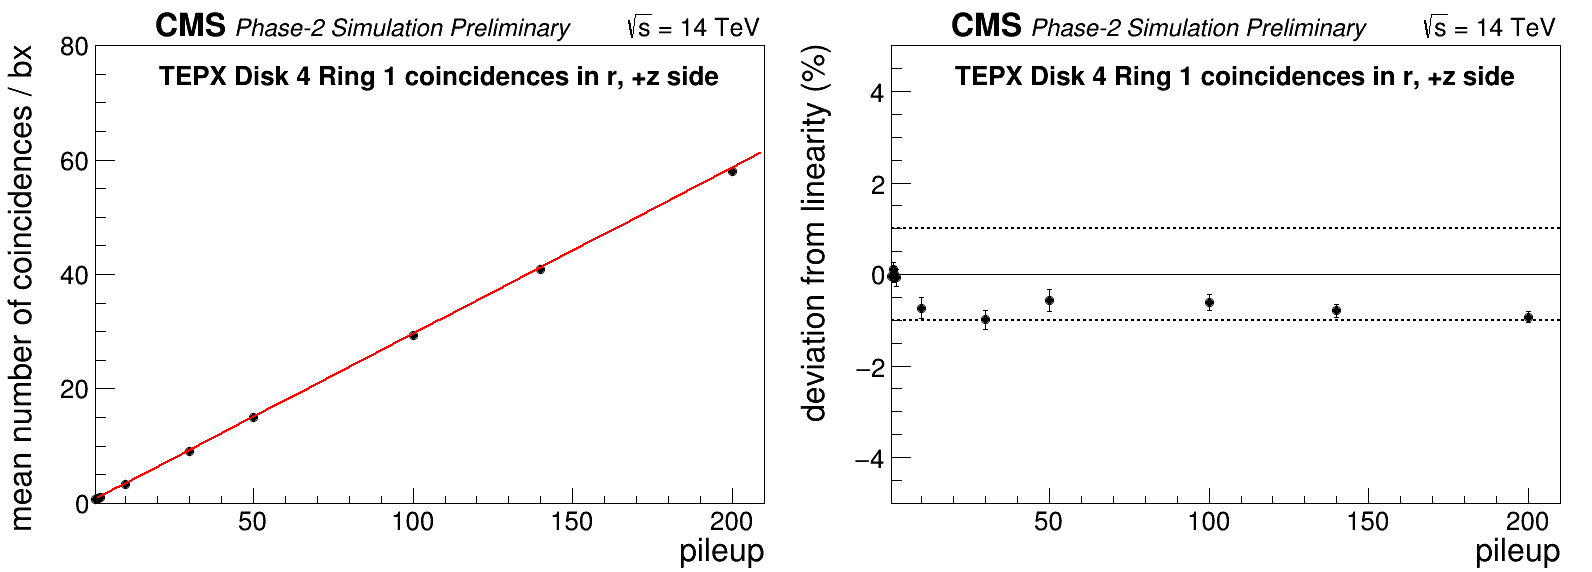
\includegraphics[width=1\columnwidth]{ashish_thesis/coincidencesinrD4R1z+.png}
  \caption[Two Fold Coincidences in r Disk 4 Ring 1 Fit And Residual]{Left: Simulated mean number of coincidences in r for TEPX +z side Disk 4 Ring 1 as a function of pileup. Right: Deviation from linearity for coincidences in r for TEPX +z side Disk 4 Ring 1. The non-linearity is calculated as the relative difference between the data points and the values of the fit function at the respective pileup value.}
  \label{fig:CMS}
\end{figure}


\begin{figure}[H]
  \centering
  \includegraphics[width=1\columnwidth]{ashish_thesis/coincidencesperringD+4.png}
  \caption[Two fold coincidences per ring Fit And Residual]{Left: Simulated mean number of coincidences in $\phi$ and r for +z side TEPX Disk 4 per ring as a function of pileup. Ring 1 has highest slope and Ring 5 has least slope. Right: Deviation from linearity for coincidences in $\phi$ and r for +z side TEPX Disk 4 per ring. Non-linearity is within 1\% for all rings over entire pileup range.}
  \label{fig:CMS}
\end{figure}

\centering
\includegraphics[width=1\textwidth]{ashish_thesis/D4R1_fake_true_ratio.png}
\caption[Disk 4 Ring 1 Fake/Total coincidences]{%
  Ratio of fake and total two fold coincidences for disk 4 ring 1.
}
\label{fig:cluster_ring_20}
\end{figure}


\begin{figure}[!htp]
\centering
\includegraphics[width=1\textwidth]{ashish_thesis/D4R5_fake_true_ratio.png}
\caption[Disk 4 Ring 5 Fake/Total coincidences]{%
  Ratio of fake and total two fold coincidences for disk 4 ring 5.
}
\label{fig:cluster_ring_21}
\end{figure}

\end{comment}

It is possible to have three fold coincidences in TEPX detector. A three-fold coincidence cluster refers to a situation where three hits are detected simultaneously within a tepx disk. The XY map of three fold coincidences is shown in Fig. \ref{fig:tepx_3foldcoin_allPU_1}.  When particles pass through the TEPX detector, they can leave behind 'traces' by interacting with the detector. These interactions are detected and measured as electrical signals. Each interaction might be seen as a 'hit' in the detector. When three of these hits occur nearly simultaneously and in a close spatial arrangement, they can form what is known as a three-fold coincidence hit originating from the same underlying event, for instance, the passage of a single particle or a single collision event. Three fold coincidences under all pileup conditions is shown in Fig.  \ref{fig:tepx_3foldcoin_allPU_2}.  With the current algorithm, three fold coincidences shows non-linearity at high pileup as shown in Fig. \ref{fig:tepx_3foldcoin_allPU_3} % and Fig.  \ref{fig:tepx_3foldcoin_lowPU}.

\begin{figure}[!htp]
  \centering
  \includegraphics[width=1\columnwidth]{ashish_thesis/tepx_threefold_coincidences.png}
  \caption[Regions in XY plane showing three fold coincidences]{X vs Y map of three fold coincidences.}
  \label{fig:tepx_3foldcoin_allPU_1}
\end{figure}


\begin{figure}[!htp]
  \centering
  \includegraphics[width=1\columnwidth]{ashish_thesis/tepx_threefold_allpu.png}
  \caption[TEPX Disk 4 Ring 2 Three Fold Coincidences]{Distribution of number of three fold coincidences for TEPX Disk 4 Ring 2 for all pileup values.}
  \label{fig:tepx_3foldcoin_allPU_2}
\end{figure}

%\begin{figure}[!htp]
 % \centering
  %\includegraphics[width=1\columnwidth]{ashish_thesis/tepx_D4_3foldcoin_allpu.png}
  %\caption[TEPX D4 All Rings Three Fold Coincidences]{Distribution of number of three fold coincidences for TEPX Disk 4 all rings for all pileup values.}
  %\label{fig:tepx_3foldcoin_allPU}
%\end{figure}

\begin{figure}[!htp]
  \centering
  \includegraphics[width=1\columnwidth]{ashish_thesis/TEPX_threefold_linearity.png}
  \caption[Disk 4 Ring 2 three Fold Coincidences Linearity]{Left: Simulated mean number of three fold coincidences for all Disk 4 all rings as a function
    of pileup. Right: Deviation from linearity for Disk 4 all rings.}
  \label{fig:tepx_3foldcoin_allPU_3}
\end{figure}


\section{Statistical precision for TEPX luminometer}
Statistical precision is another uncertainty that need to be considered for precise luminosity measurement. It must be kept minimal to achieve 1 $\%$ accuracy for HL-LHC luminosity measurement.

Relative statistical uncertainty in $\%$ = $\frac{\sqrt{N}}{N} \times 100$ \\

where N = (Number of counts per event)$\times$(Trigger Frequency)$\times$(Time Integration period). 


\begin{table}[htbp]
  \centering
  \caption[Expected stat. precision of TEPX under low pileup] {Expected statistical precision (in $\%$) in head-on collisions during typical vdM conditions with pileup of 0.5 for TEPX clusters and two fold coincidences over different integration time period.}
\begin{tabular}{lcccc}
vdM (PU 0.5) & Readout Rate (kHz) & 1 bx, 1s & 1 bx, 30s & 100 bx, 30s\\
\hline
TEPXD4R1 Clusters&1000&1.82&0.332 & 0.0332\\
TEPXD4R1 2x Coincidences in phi &1000&5.98&1.09 & 0.109\\
TEPXD4R1 2x Coincidences in r &1000&11.1&2.02 & 0.202\\
TEPXD4R1 2x Coincidences &1000&5.27&0.962 & 0.0962\\
TEPX Clusters&500&0.709&0.129 & 0.0129\\
TEPX 2x Coincidences in phi &500&2.65&0.485 & 0.0485\\
TEPX 2x Coincidences in r &500&4.59&0.838 & 0.0838\\
TEPX 2x Coincidences &500&2.3&0.42 & 0.042\\
\end{tabular}
\end{table}


\begin{table}[htbp]
\centering
\caption[Expected stat. precision of TEPX under high pileup]{Expected statistical precision (in $\%$) in head-on collisions during physics conditions with pileup of 200 for TEPX clusters and two fold coincidences over different integration time period.}
\begin{small} % this command will decrease the font size
\begin{tabular}{lcccc}
Algorithm & Readout Rate (kHz) & 1 bx, 1s & 2500 bx, 1s & 2500 bx, 1 LS \\
\hline
TEPXD4R1 Clusters & 825 & 0.1 & 0.002 & 0.000414 \\
TEPXD4R1 2x Coincidences in phi & 825 & 0.329 & 0.00659 & 0.00136 \\
TEPXD4R1 2x Coincidences in r & 825 & 0.61 & 0.0122 & 0.00252 \\
TEPXD4R1 2x Coincidences & 825 & 0.29 & 0.0058 & 0.0012 \\
TEPX Clusters & 75 & 0.0915 & 0.00183 & 0.000379 \\
TEPX 2x Coincidences in phi & 75 & 0.343 & 0.00685 & 0.00142 \\
TEPX 2x Coincidences in r & 75 & 0.593 & 0.0119 & 0.00245 \\
TEPX 2x Coincidences & 75 & 0.297 & 0.00594 & 0.00123 \\
\end{tabular}
\end{small}
\end{table}


\section{Summary of the planned upgrade schedule}

The Phase II upgrade of the CMS detector is a major project that will take several years to complete. The design and development of the upgraded components is currently underway, and the installation of the new detectors and electronics is scheduled to take place over the next few years. The commissioning and testing phase will be critical to ensure that the upgraded detector is functioning properly, and full operation of the upgraded CMS detector is expected to begin in 2026. Planned upgrade schedule for the Phase II upgrade of the CMS detector:

\begin{itemize}

\item 2018-2024: Design and development of the upgraded components, including the new pixel and strip detectors, timing layer, and data acquisition system.

\item 2022-2023: Installation of the new carbon-fiber support structure for the upgraded tracker.

\item 2024-2026: Installation of the new detectors and electronics in the CMS detector, including the pixel and strip detectors, timing layer, and data acquisition system.

\item 2027-2028: Commissioning and testing of the upgraded detector.

\item 2029: Full operation of the upgraded CMS detector.

\end{itemize}

